\documentclass[usenames,dvipsnames]{beamer}
\usepackage[spanish]{babel}
%\usepackage[latin1]{inputenc}
\usepackage[utf8]{inputenc}
\usepackage{graphicx}
\usepackage{booktabs}

\usepackage{multicol}
\usepackage{multirow}
\useoutertheme{tree}

\usepackage{appendixnumberbeamer}

% ******************flechas
\usepackage{times}
\usepackage{tikz}
\usepackage{amsmath}
\usepackage{verbatim}
\usetikzlibrary{arrows,shapes}

%********************


% %nro de pagina
% \usepackage{fancyhdr}
% \fancypagestyle{plain}{% en los inicios de capitulo
% % 	\fancyhead{} % get rid of headers
% % 	\renewcommand{\headrulewidth}{0pt} % and the line
% 	\fancyfoot[C]{\thepage} % add page number
% }
%\usepackage{color}
%\usepackage[usenames,dvipsnames,svgnames,table]{xcolor}

%\usetheme{Dresden}
\usetheme[titleformat=smallcaps, numbering=fraction, block=fill]{metropolis}
%\setcounter{tocdepth}{1}
%\usecolortheme{dolphin}
% \useoutertheme{shadow}
% \useinnertheme{rectangles}

% *************************** Caratula


\title[Instituto Sabato]{Diseño y caracterización de esponjas pseudoelásticas}
%\subtitle{}
\author[Prado L.H.]
{
Lucia Helena \textsc{Prado} \\
\\
{\tiny directora:} {\small Dra. Graciela \textsc{Bertolino}}\\
{\tiny codirector:} {\small Pierre \textsc{Arneodo Larochette}}\\
{\tiny tutor:} {\small Dr. Alfredo \textsc{Hazarabedian}} \\
}
\institute{Instituto Sabato 
           \and División Física de Metales - Centro Atómico Bariloche  }
\date{26/07/2017}


% ************************* Para poner indice antes de cada seccion con dos columnas
 
 
% \AtBeginSection{
% \begin{frame}
%   \frametitle{Índice}
% %   \begin{multicols}{1}
%   \tableofcontents[currentsection]
% %   \end{multicols}
% \end{frame}
% }
% 
% \AtBeginSubsection{
% \begin{frame}
% %   \frametitle{Índice}
%   \begin{multicols}{1}
%   \tableofcontents[currentsection,currentsubsection]
% %   \end{multicols}
% \end{frame}
% }
 %****************************8 Con dos columnas

 %   \AtBeginSection{ 
% \begin{frame} 
%   \frametitle{Índice}
%   \tableofcontents[currentsection]
% \end{frame}
% }
% 
% \AtBeginSubsection{ 
% \begin{frame}
%   \frametitle{Índice}
%   \tableofcontents[currentsection,currentsubsection]
% \end{frame}
% }
\DeclareFontEncoding{LS1}{}{}
\DeclareFontSubstitution{LS1}{stix}{m}{n}
\DeclareRobustCommand{\diameter}{%
  \text{\usefont{LS1}{stixscr}{m}{n}\symbol{"60}}%
}

% *****************************************8 Diapos 
% \addtocounter{framenumber}{-1}
%\insertframenumber/\inserttotalframenumber
% saca el menu feo
\setbeamertemplate{navigation symbols}{}

 \begin{document}

 %*********************************************************Flechas
 % For every picture that defines or uses external nodes, you'll have to
% apply the 'remember picture' style. To avoid some typing, we'll apply
% the style to all pictures.
\tikzstyle{every picture}+=[remember picture]

% By default all math in TikZ nodes are set in inline mode. Change this to
% displaystyle so that we don't get small fractions.
\everymath{\displaystyle}
%***********************************************************************
 
 
  \frame{\titlepage}
%  
% \begin{frame}
%     \frametitle{Marsupiales}
%     Canguro, Koala, Wombat...
% \end{frame}
% 
% 
% \begin{frame}
%   \frametitle{Marsupiales}
%   \begin{block}{Marsupiales en Australia}
%   Koala, Canguro, Wombat...
%   \end{block}
%       
%   \begin{block}{Marsupiales fuera de Australia}
%   Oposum, Zarigüella...
%   \end{block}
% \end{frame}
% 
% 
% \begin{frame}
%   \frametitle{Animales}
%   \begin{columns}[t]
%     \column{0.5\textwidth}
%     Algunos mamíferos marinos:
%  
%     Ballena, Narval, Cachalote...
% 
%     \column{0.5\textwidth}
%     Y algunos má
%     s:
%  
%     Morsa, León marino, Foca...
%   \end{columns}
% \end{frame}
% 
% 
% \begin{frame}
%   \frametitle{Flores}
%   \begin{itemize}
%   \item<1->{Rosa}
%   \item<2->{Azucena}
%   \item<3->{Margarita}
%   \end{itemize}
% \end{frame}
% 
% 
% \begin{frame}
%   \frametitle{Preguntas}
%   \begin{itemize}
%   \item \alert<1>{¿Cuáles ponen huevos?}
%   \item \alert<3>{¿Cuáles tienen veneno?}
%   \end{itemize}
%      
%   Armadillo, \alert<2,4>{Ornitorrinco}, \alert<2>{Equidna}, Pangolín, Erizo.
% \end{frame}


% ******************
%\section{Introducción}

%%%%%%%%%%%%%%%%%%%%%%%%%%%%%%%%%%%%%%%%%%%%%%%%%%%%%%%%%%%%%%%%%%%%%%% INTRODUCCION
\begin{frame}
\frametitle{Introducción}
\begin{columns}
\column{0.5\textwidth} 
\begin{block}{
Esponjas pseudoelásticas \\
\quad \quad \quad \quad $=$ \\
\quad Aleación de CuZnAl \\
\quad \quad \quad \quad $+$ \\
\quad Estructura celular}
\end{block}
\vfill
\begin{center}

\includegraphics[width=0.5\columnwidth]{img/Esponja.png}
\end{center}
\column{0.5\textwidth}

\begin{block}{
 Organización del trabajo:}
\end{block}
\begin{itemize}
 \item Introducción teórica
 \item Modificación del tamaño de grano
 \item Integridad estructural y seguimiento de la transformación
 \item Conclusiones
\end{itemize}

\end{columns}
\end{frame}

%%%%%%%%%%%%%%%%%%%%%%%%%%%%%%%%%%%%%%%%%%%%%%%%%%%%%%%%%%%%%%%%%%%%%%%%%%%%%%%%%%%%%%%%%%%%%%%%%%%%%%%%%%%%%%%%

\begin{frame}

\frametitle{Transformaciones de la aleación}
 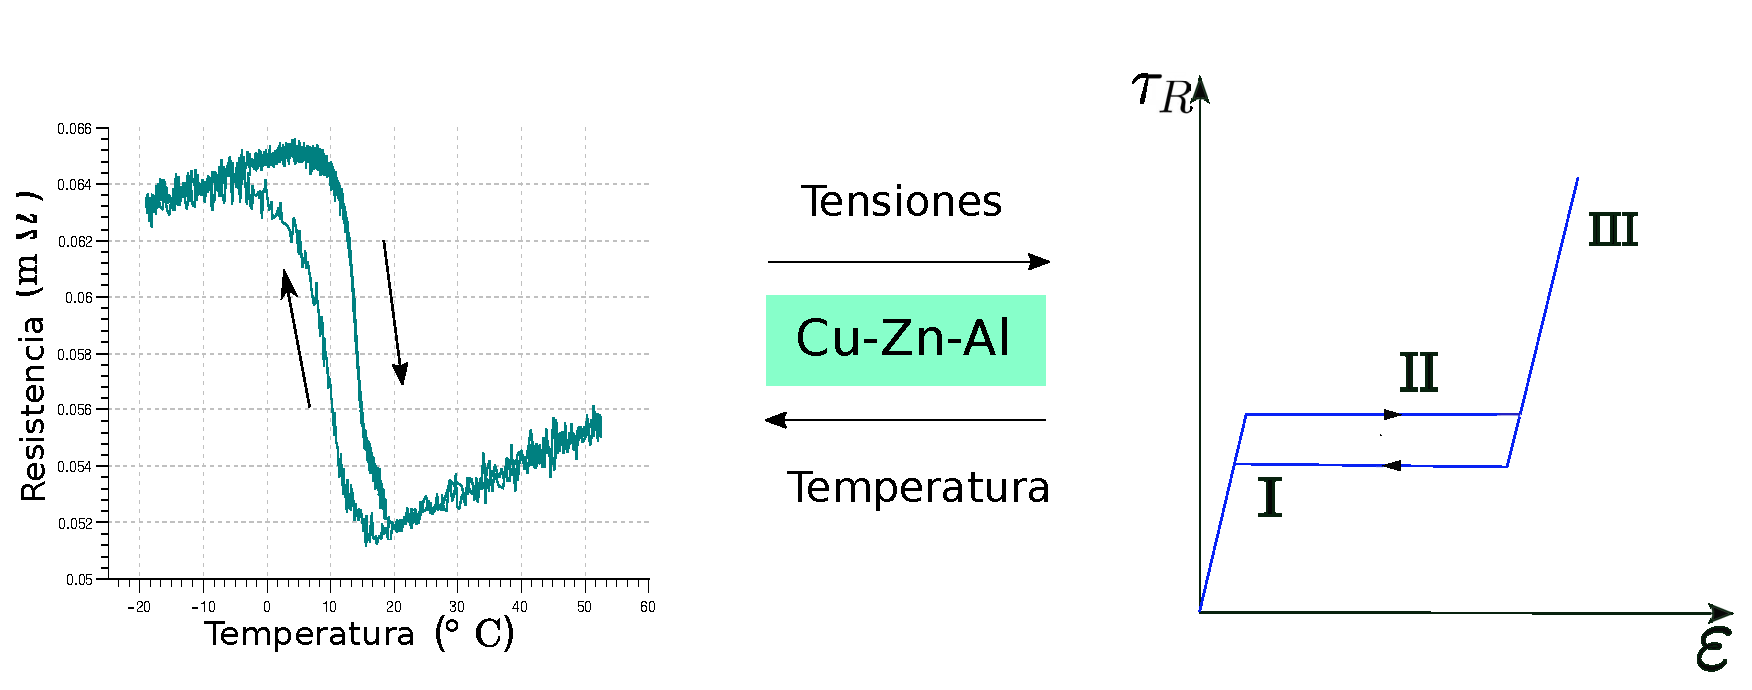
\includegraphics[width=\textwidth]{img/intro/Intro.eps}
\end{frame}







% \begin{frame}
% \frametitle{Memoria de forma}
% 
%  \begin{itemize}
%   \item Forma inicial en estado austenítico
%   \item Enfriamiento a $T<M_{s}$
%   \item Deformación en estado martensítico
%   \item Calentamiento a $T>A_{f}$
%  \end{itemize}
% 
% 
% \begin{center}
% 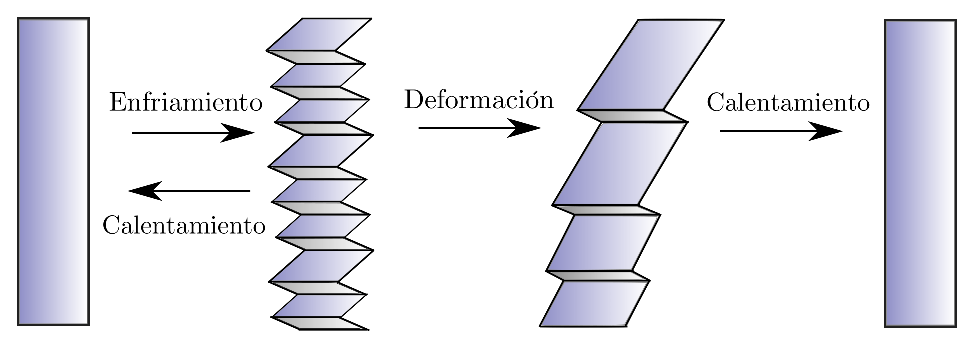
\includegraphics[width=0.9\textwidth]{img/intro/Trans.eps} 
% % 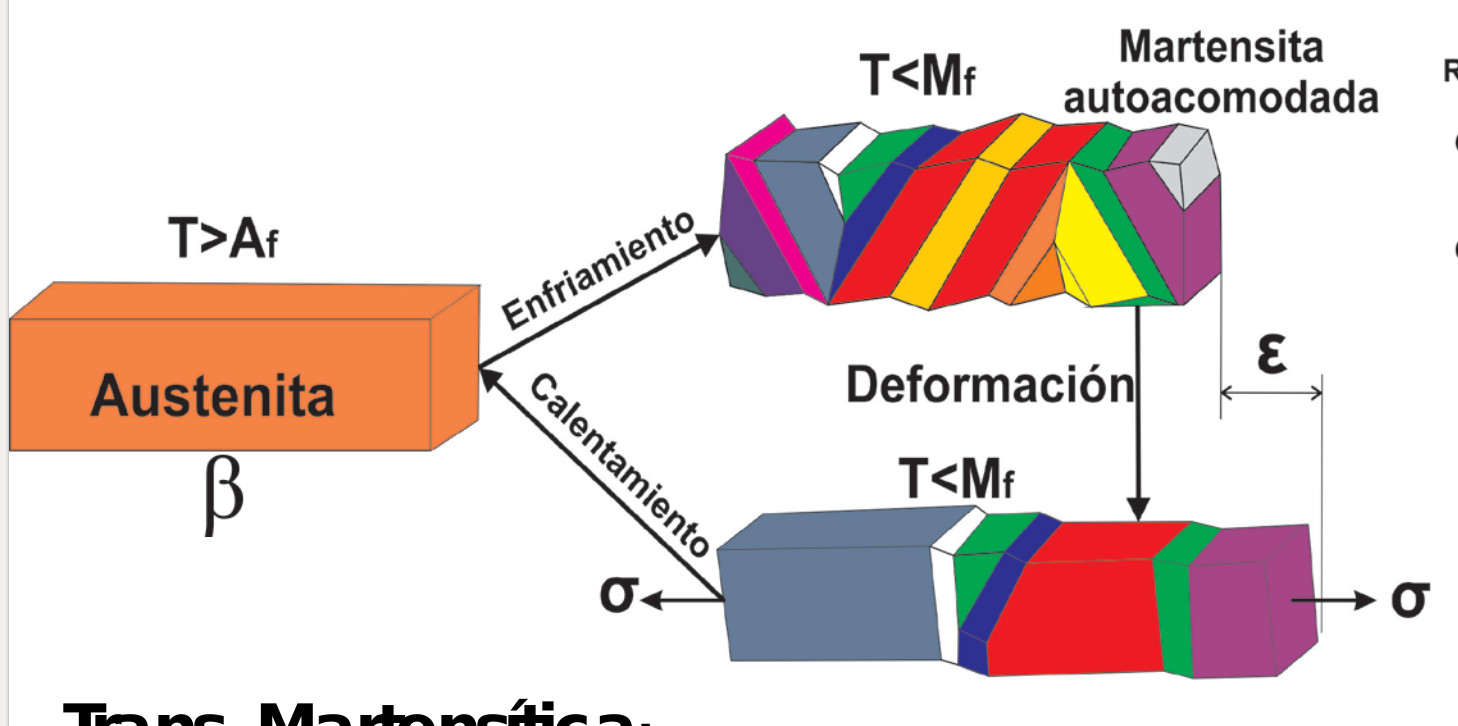
\includegraphics[width=0.8\textwidth]{img/intro/memoria.jpg}
% \end{center}
% 
% % Cosas que juegan en contra:
% % \begin{itemize}
% %   \item Envejecimiento y estabilización
% %   \item Anclaje entre placas de martensita
% %  \end{itemize}
% 
% \end{frame}

%%%%%%%%%%%%%%%%%%%%%%%%%%%%%%%%%%%%%%%%%%%%%%%%%%%%%%%%%%%%%%%%%%%%%%%%%%%%%%%%%%%%%%%%%%%%%%%%%%%%%%%%%%%%%%%%%*************************

%  \begin{frame}
%  \frametitle{Transformación martensítica}
% 
% \begin{columns}
%  
% \column{0.5\textwidth}
% 
% % \begin{block}{Características}
% %  \begin{itemize}
% %   \item En estado sólido
% %   \item Sin difusión
% %   \item De primer orden
% %  \end{itemize}
% % \end{block}
%  
% \begin{block}{Formas de transformación}
%   \begin{itemize}
%   
%   \item Inducida térmicamente ($M_s$ y $M_f$)
% 
%   \item Inducida por tensiones (Strain Induced Martensite)
%  \end{itemize}
% \end{block}
% 
% \column{0.5\textwidth}
% 
% 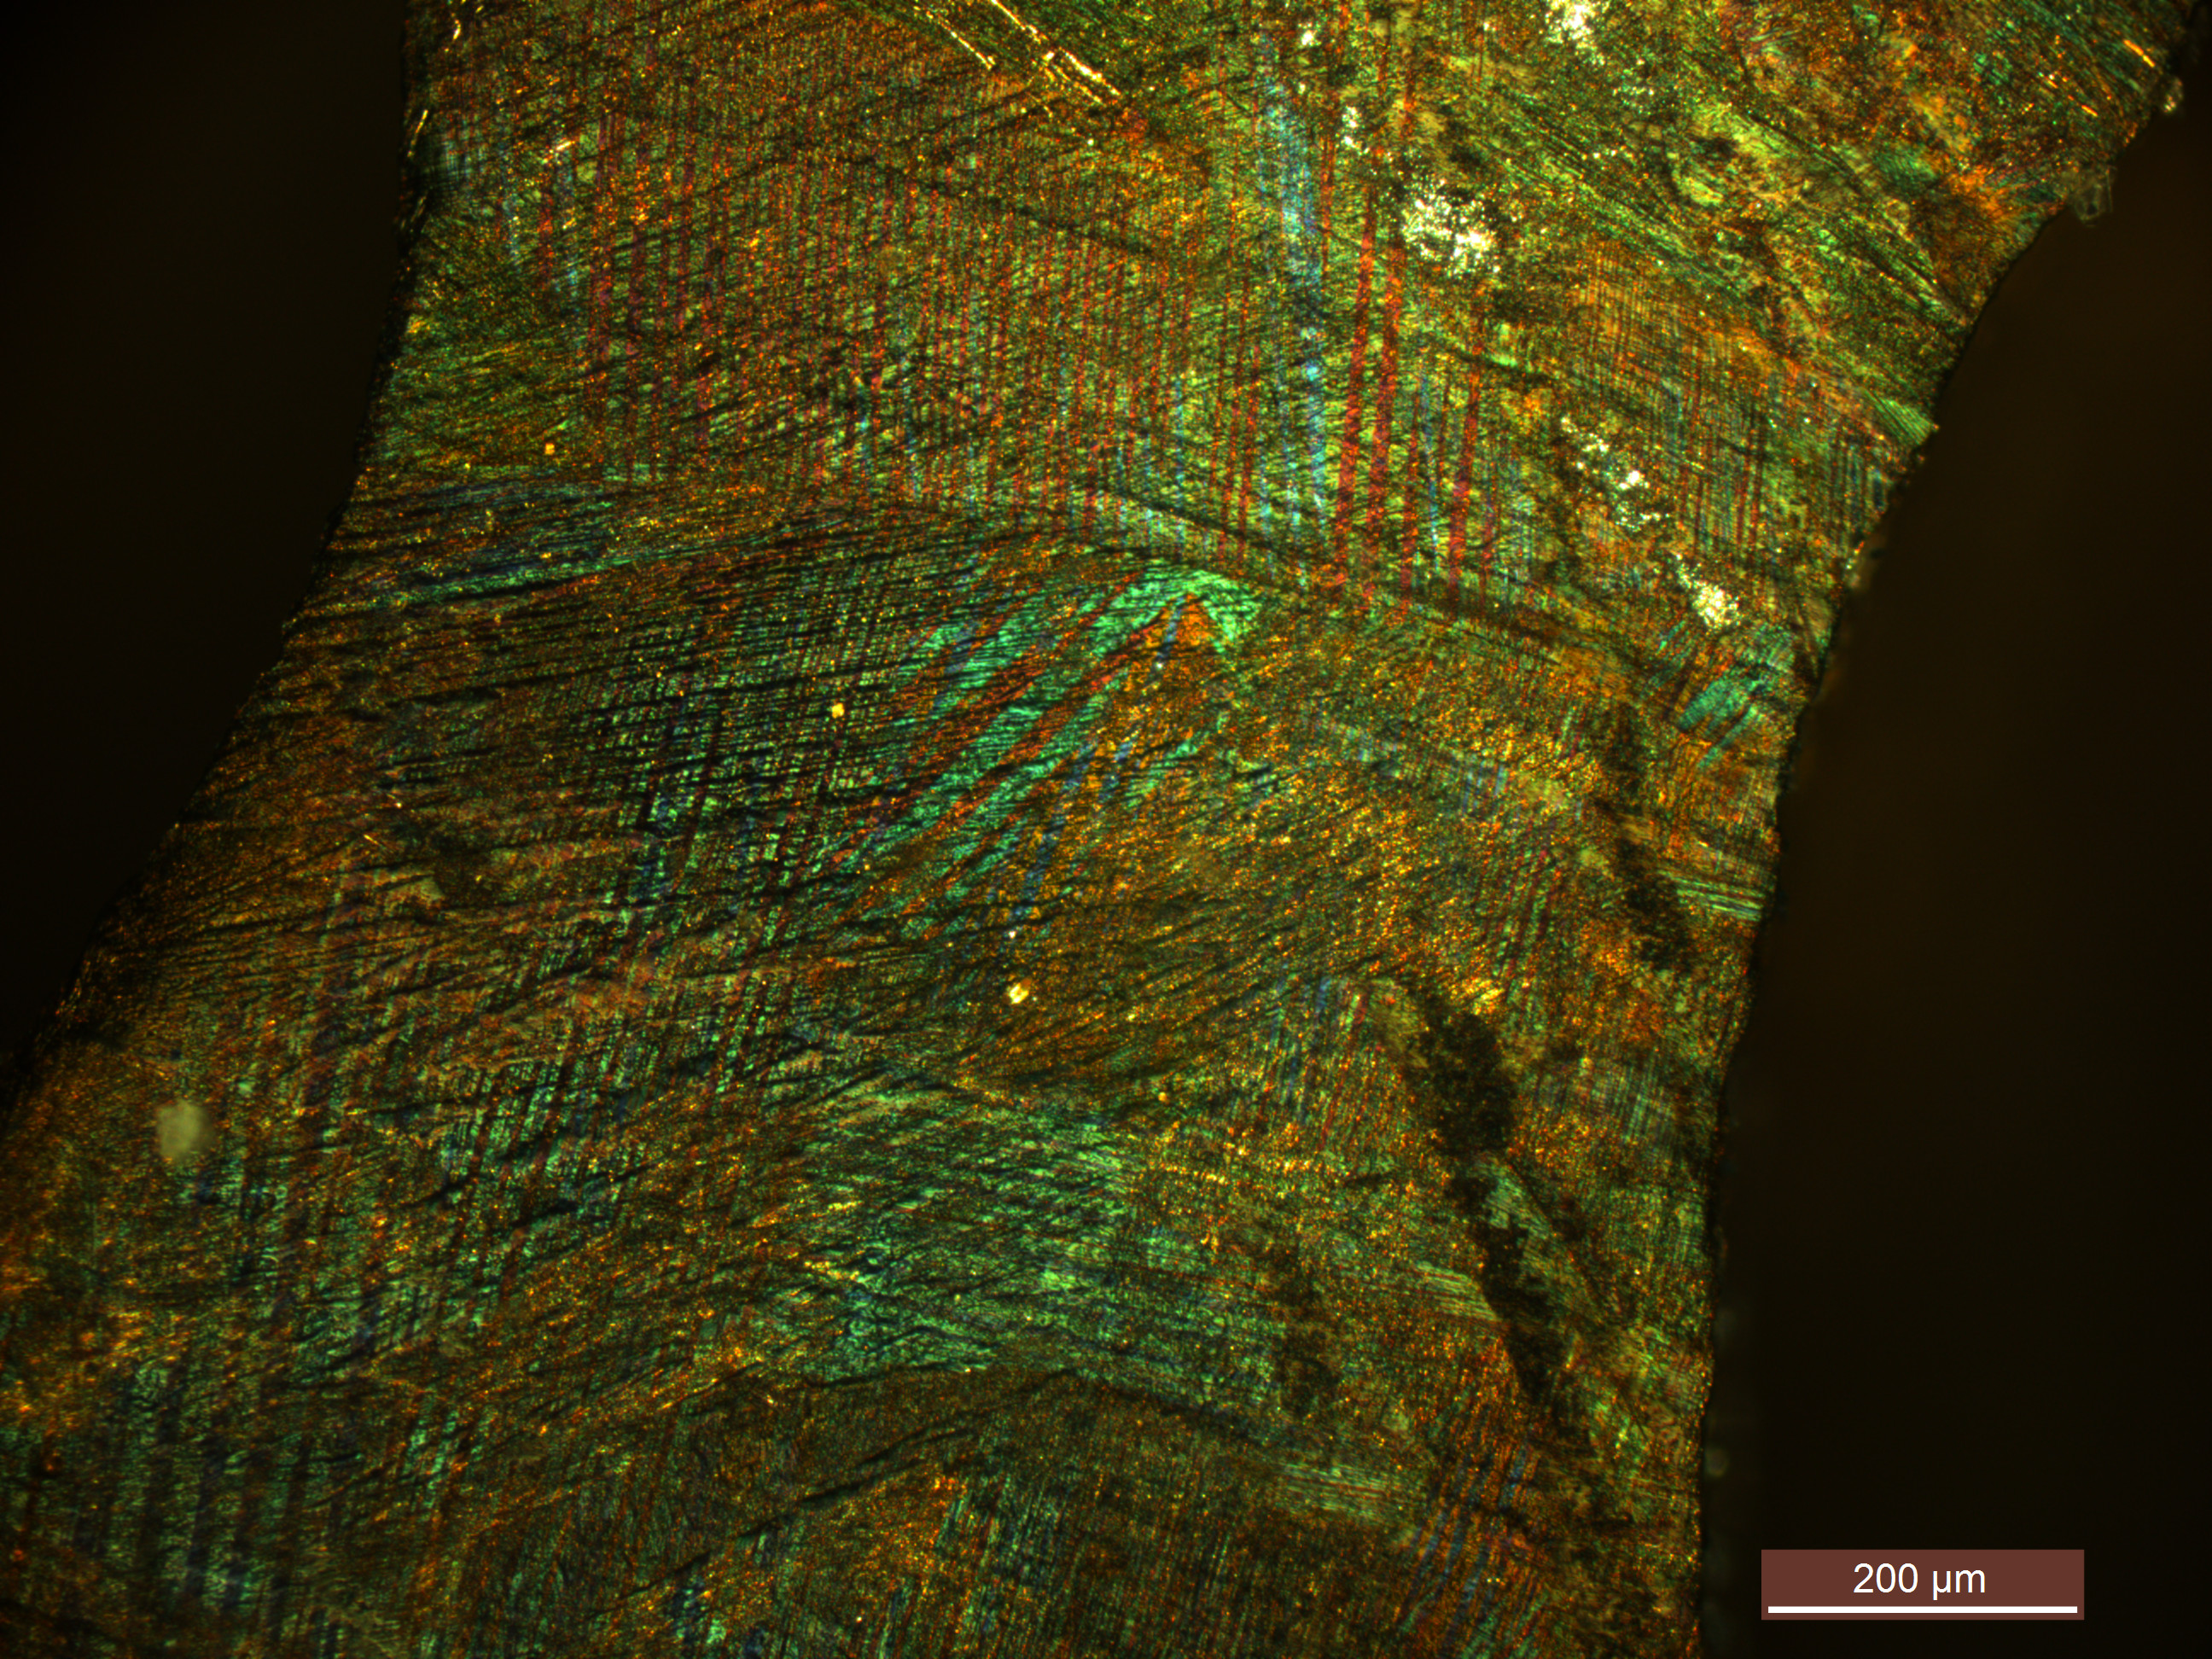
\includegraphics[width=\columnwidth]{img/intro/EspAMicro1.jpg}
% 
% \end{columns}
%  
% \end{frame}

%%%%%%%%%%%%%%%%%%%%%%%%%%%%%%%%%%%%%%%%%%%%%%%%%%%%%%%%%%%%%%%%%%%%%%%%%%%%%%%%%%%%%%

%  \begin{frame}
%  \frametitle{Transformación martensítica}
% 
% \begin{columns}
%  
% \column{0.5\textwidth}
% 
% \begin{block}{Características}
%  \begin{itemize}
%   \item En estado sólido
%   \item Sin difusión
%   \item De primer orden
%  \end{itemize}
% \end{block}
%  
% \begin{block}{Formas de transformación}
%   \begin{itemize}
%   \item Inducida térmicamente ($M_s$ y $M_f$)
%   \item \alert<1>{Inducida por deformación? (Strain Induced Martensite)}
%  \end{itemize}
% \end{block}
% 
% \column{0.5\textwidth}
% 
% 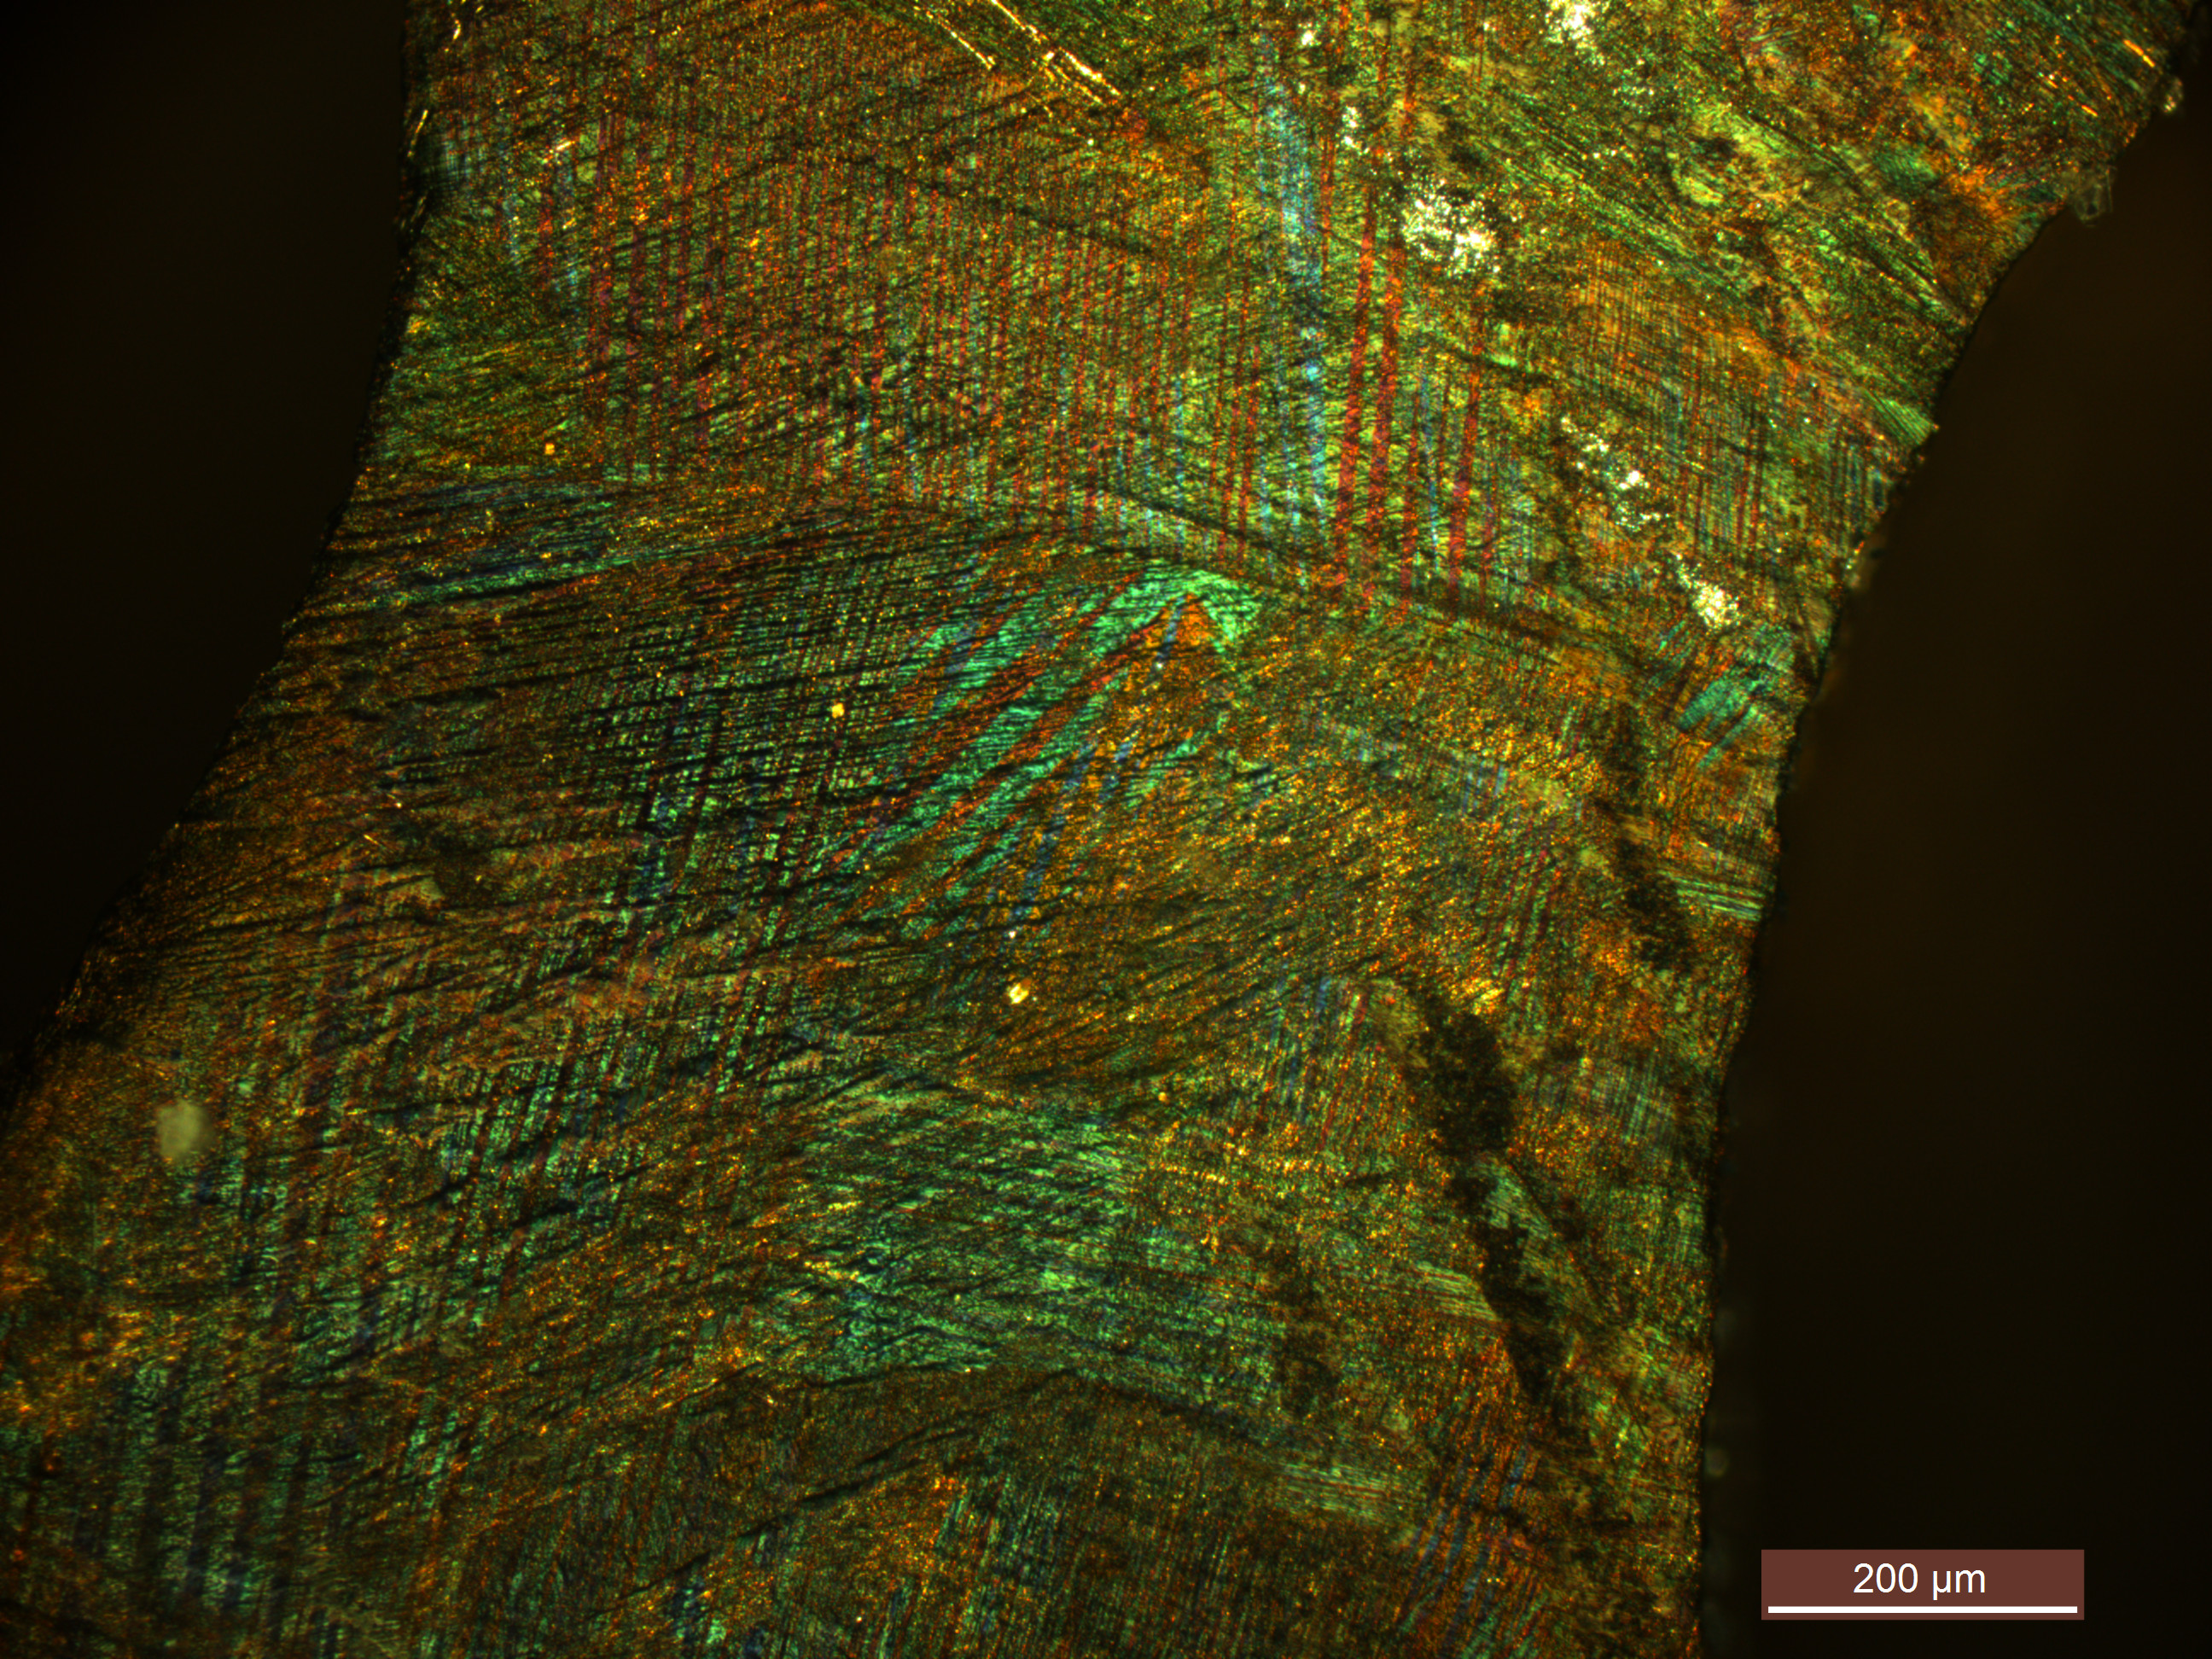
\includegraphics[width=\columnwidth]{img/intro/EspAMicro1.jpg}
% 
% \end{columns}
%  
% \end{frame}

%%%%%%%%%%%%%%%%%%%%%%%%%%%%%%%%%%%%%%%%%%%%%%%%%%%%%%%%%%%%%%%%%%%%%%%%%%%%%%%%%%%%%%%%%%%%%%%%%%%%%%%%%%%%%%%%% 

% \begin{frame}
% \frametitle{Transformación martensítica Inducida por Deformación}
% 
% \begin{figure}
% \begin{tikzpicture}
% \pgftext{%
%  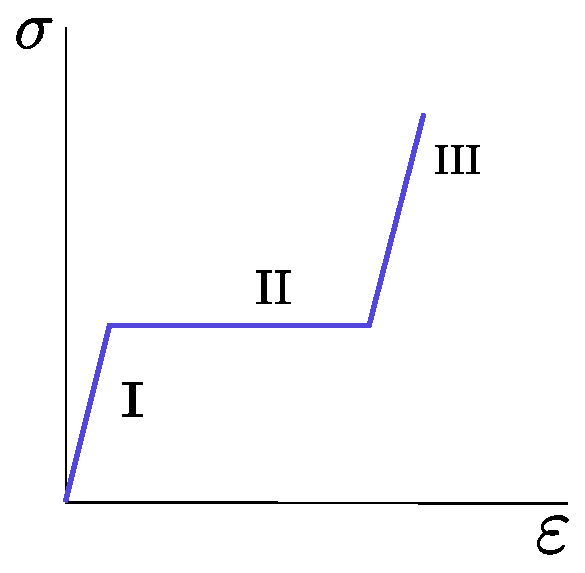
\includegraphics[width=0.4\textwidth]{img/intro/SigmavsDef.eps}
% }%
% 
% \node (I) at (-1.2,-0.9) {};
% \node (II) at (0, 0) {};
% \node (III) at (1.5, 1) {};
% \node[align=right] (It)   at (5.25, -1.3) {Deformación elástica de $\beta$};
% \node[align=right] (IIt)  at (6,0) {Formación y crecimiento \\ de placas de martensita};
% \node[align=right] (IIIt) at (4.8, 1.4) {Deformación elástica \\ de la martensita};
% % 
% \path[->]<1-> (I) edge [green, dashed, thick] (It);
% \path[->]<1-> (II) edge [green, dashed, thick] (IIt);
% \path[->]<1-> (III) edge [green, dashed, thick] (IIIt);
% 
% \end{tikzpicture}
% \end{figure}
% 
%  
% \end{frame}
%%%%%%%%%%%%%%%%%%%%%%%%%%%%%%%%%%%%%%%%%%%%%%%%%%%%%%%%%%%%%%%%%%%%%%%%%%%%%%%%%%%%%%%%%%%%

%%%%%%%%%%%%%%%%%%%%%%%%%%%%%%%%%%%%%%%%%%%%%%%%%%%%%%%%%%%%%%%%%%%%%%%%%%%%%%%%%%%%%%%%%%%%%%%%%%%%%%%%%%%%%%%%%%%%%

\begin{frame}
\frametitle{Transformación en Monocristales y Policristales}

\begin{columns}
\column{0.6\textwidth}

\begin{block}{Tensión Resuelta}
\begin{equation*}
 \tau_{R}= \sigma cos(\lambda)cos(\phi)
\end{equation*}

\begin{center}
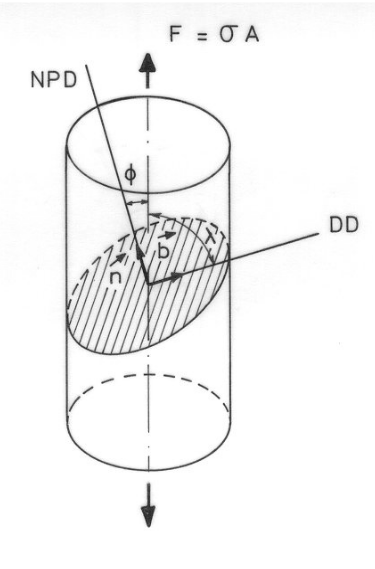
\includegraphics[width=0.5\columnwidth]{img/intro/tension.png}
\end{center}

\end{block}

\column{0.4\textwidth}

%\pause
\begin{block}{Monocristal}
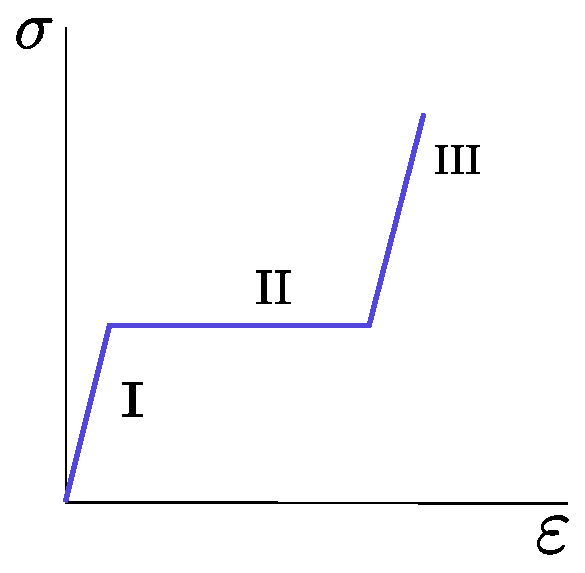
\includegraphics[height=0.35\textheight]{img/intro/SigmavsDef.eps} 
\end{block}

%\pause
\begin{block}{Policristal}
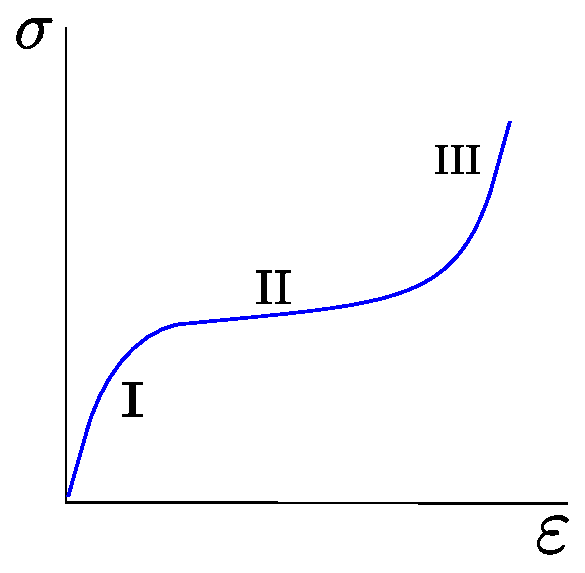
\includegraphics[height=0.35\textheight]{img/intro/SigmavsDefPoli.eps}
\end{block}

\end{columns}

% \end{center}
% \end{multicols}
 
\end{frame}
%%%%%%%%%%%%%%%%%%%%%%%%%%%%%%%%%%%%%%%%%%%%%%%%%%%%%%%%%%%%%%%%%%%%%%%%%%%%%%%%%%%%%%%%%%%%%%%%%%%%%%%%%%%%%%%%
\begin{frame}
\frametitle{Variaciones en los parámetros de transformación}

\begin{columns}
\column{0.4\textwidth}

\begin{block}{Clausius-Clapeyron}
\begin{equation*}
 \frac{d \tau_{R}}{dT}=\frac{\Delta S}{\Delta V} 
\end{equation*}
\end{block}

\begin{itemize}
 \item $\uparrow T \rightarrow \, \uparrow \tau_{R}$
 \item $\tau_{R} = 0  \rightarrow T=M_{s}$
\end{itemize}

\column{.4\textwidth}
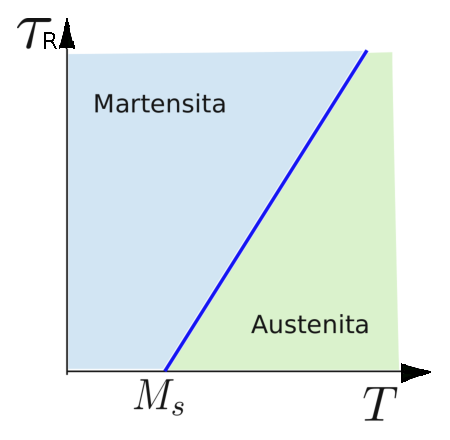
\includegraphics[width=\columnwidth]{img/intro/Clapeyron.eps}

\end{columns}

% \begin{figure}
% \begin{tikzpicture}
% \node[align=left] (It)   at (0, 0)[rectangle, draw, red] {Falta variación de ancho de la histéresis};
% \end{tikzpicture}
% \end{figure}

\end{frame}


% \begin{frame}
% 
% \frametitle{Pseudoplasticidad}
% 
% \begin{figure}
% \begin{tikzpicture}
% 
% \node (I) at (0,0) {};
% \node[align=left] (It)   at (0,1) {Gasto de energía debido a la fricción en el movimiento \\ de interfases y creación de defectos.};
% % 
% \path[->]<1-> (I) edge [dashed] (It);
% 
% \end{tikzpicture}
% \end{figure}
% 
% \begin{columns}
% \column{0.4\textwidth}
% 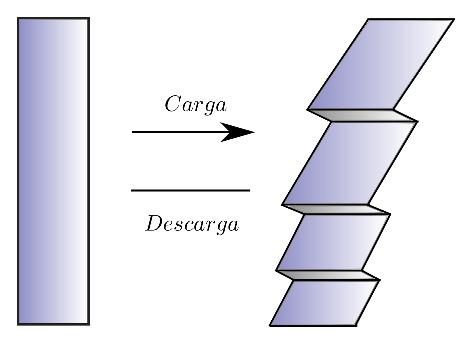
\includegraphics[width=\columnwidth]{img/intro/HisteresisEsquema.eps}
% \column{0.4\textwidth}
% 
% 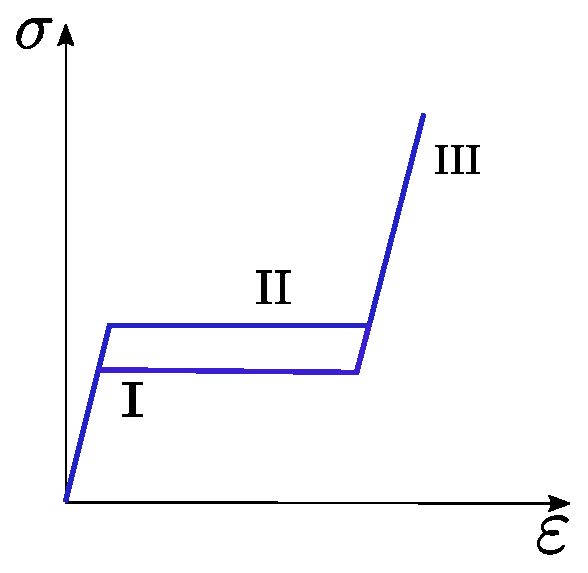
\includegraphics[width=\columnwidth]{img/intro/Histeresis.eps}
% 
% \end{columns}
% 
% \end{frame}

%%%%%%%%%%%%%%%%%%%%%%%%%%%%%%%%%%%%%%%%%%%%%%%%%%%%%%%%%%%%%%%%%%%%%%%%%%%%%%%%%%%%%%%%%%%%%%%%%%%%%%%%%%%%%%%%%%%%%%%%%%%%%%%%%%%%%%%%%%%


\begin{frame}

\frametitle{Disipación de energía}

\begin{figure}
\begin{tikzpicture}

\node (I) at (3,1.5) {};
\node[align=left] (It)   at (0,5) {Disipación de energía debido a la fricción en el movimiento \\ de interfases y creación de defectos.};
% 
\draw[green, very thick, dashed] (-5.2,4.4) -- (5.2,4.4) -- (5.2,5.6) -- (-5.2,5.6) -- (-5.2,4.4);
\path[->]<1-> (It) edge [bend left, very thick, green, dashed] (I);


% 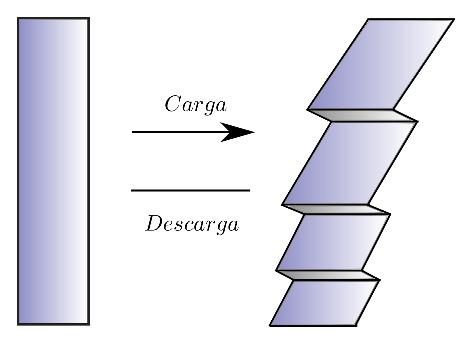
\includegraphics[width=0.4\columnwidth]{img/intro/HisteresisEsquema.eps}
\node[anchor=south west,inner sep=0] (image) at (-4,0) {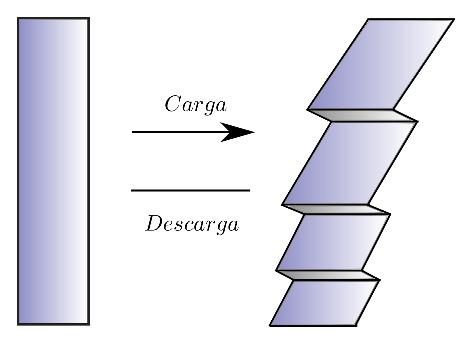
\includegraphics[width=0.4\textwidth]{img/intro/HisteresisEsquema.eps}};
\node[anchor=south west,inner sep=0] (image) at (1,0) {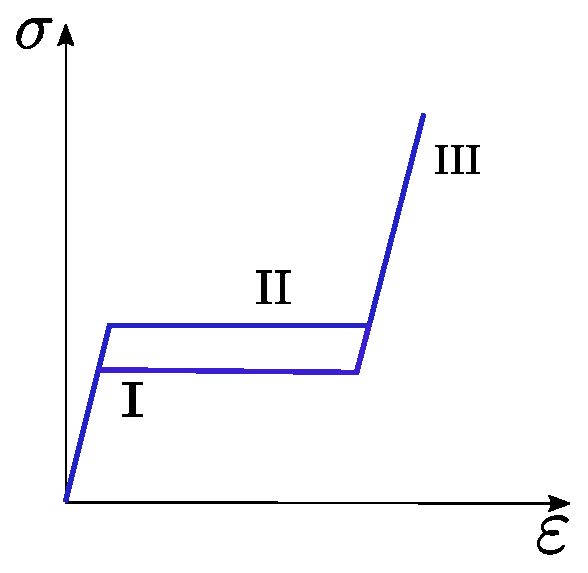
\includegraphics[width=0.4\textwidth]{img/intro/Histeresis.eps}};
%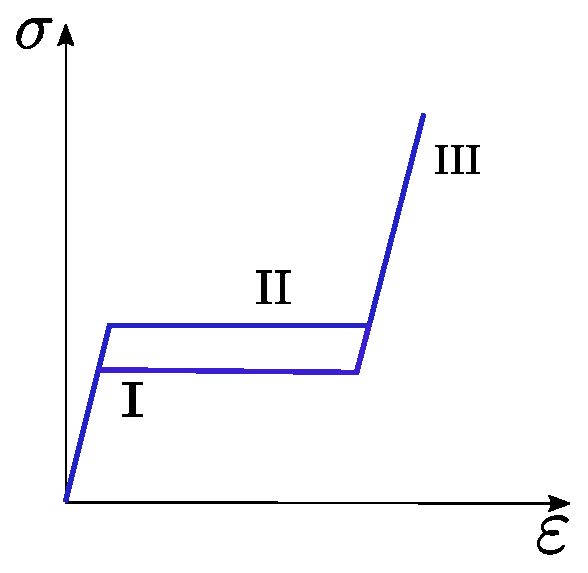
\includegraphics[width=0.4\columnwidth]{img/intro/Histeresis.eps}


\end{tikzpicture}
\end{figure}






\end{frame}

%%%%%%%%%%%%%%%%%%%%%%%%%%%%%%%%%%%%%%%%%%%%%%%%%%%%%%%



%%%%%%%%%%%%%%%%%%%%%%%%%%%%%%%%%%%%%%%%%%%%%%%%%%%%%%



% ************************ 

% \begin{frame}
% \frametitle{Aleación Cu-Zn-Al}
% \begin{center}
% 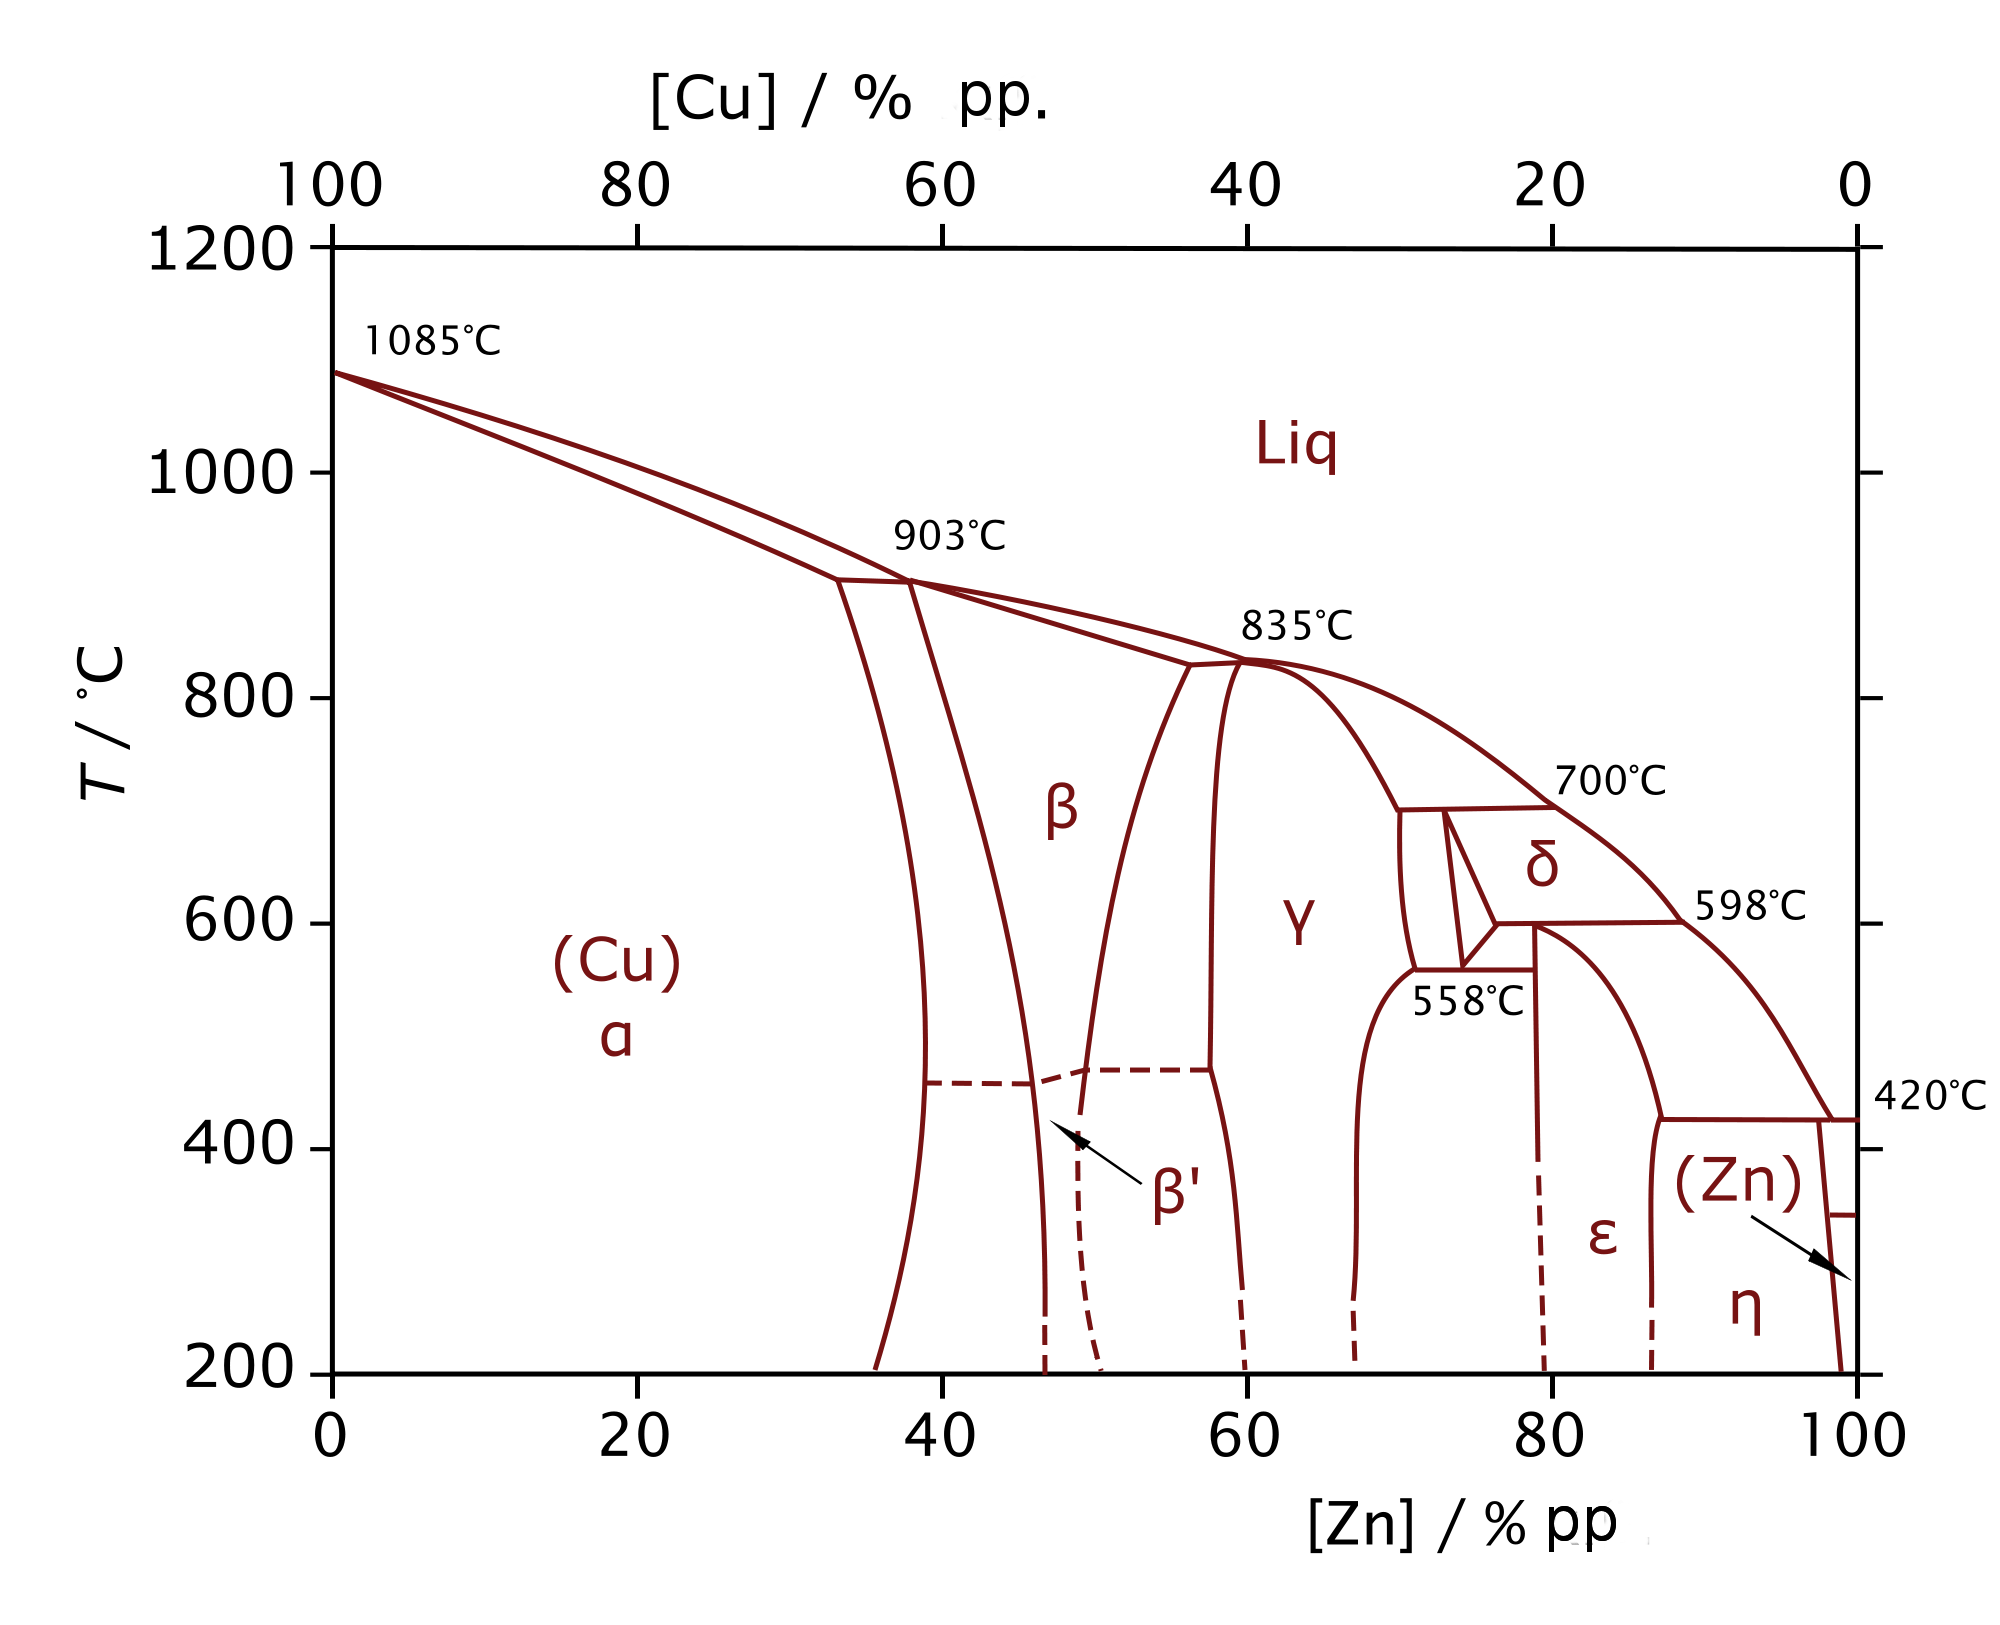
\includegraphics[width=0.6\textwidth]{img/intro/CuZn.png} 
% \end{center}
% 
%  
% % \begin{equation*}
% %  \beta \rightarrow B2 \rightarrow L2_1 \rightarrow 18R 
% % \end{equation*}
% 
% 
% \begin{figure}
% \begin{tikzpicture}
% % \pgftext{%
% %  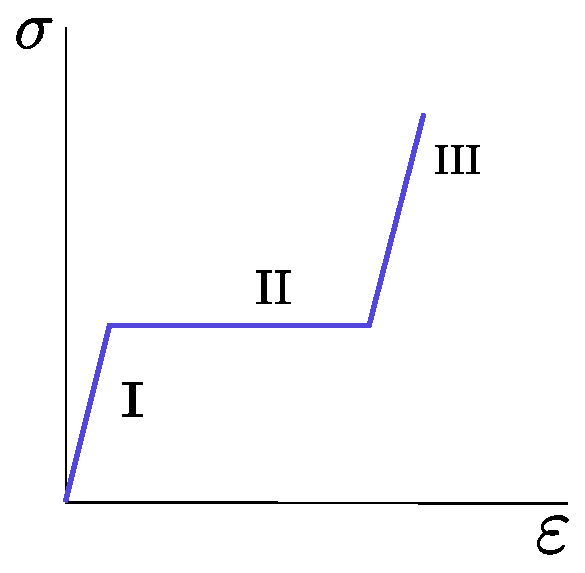
\includegraphics[width=0.4\textwidth]{img/intro/SigmavsDef.eps}
% % }%
% 
% \node (I) at (-1.2,-0.9) {};
% \node (II) at (0, 0) {};
% \node (III) at (1.5, 1) {};
% \node[fill=green!10,align=right,circle,draw] (It)   at (0, 1) {$\beta$};
% \node[fill=green!10,align=right,circle,draw] (IIt)  at (2,1) {$B2$};
% \node[fill=green!10,align=right,circle,draw] (IIIt) at (4,1.3) {$L2_1$};
% \node[fill=green!10,align=right,circle,draw] (IIIIt) at (6,1.3) {$18R$};
% \node[fill=green!10,align=right,circle,draw] (IIIIIt) at (4,0.3) {$9R$};
% % 
% \path[->]<1-> (It) edge [blue, thick] (IIt);
% \path[->]<1-> (IIt) edge [blue, thick] (IIIt);
% \path[->]<1-> (IIIt) edge [blue, thick] (IIIIt);
% \path[->]<1-> (IIt) edge [blue, thick] (IIIIIt);
% %\path[->]<1-> (IIt) edge [dashed] (IIIIIt);
% 
% \end{tikzpicture}
% \end{figure}
% \end{frame}

%*************************
% 
% \begin{frame}
% \frametitle{Aleación Cu-Zn-Al}
% \begin{center}
% 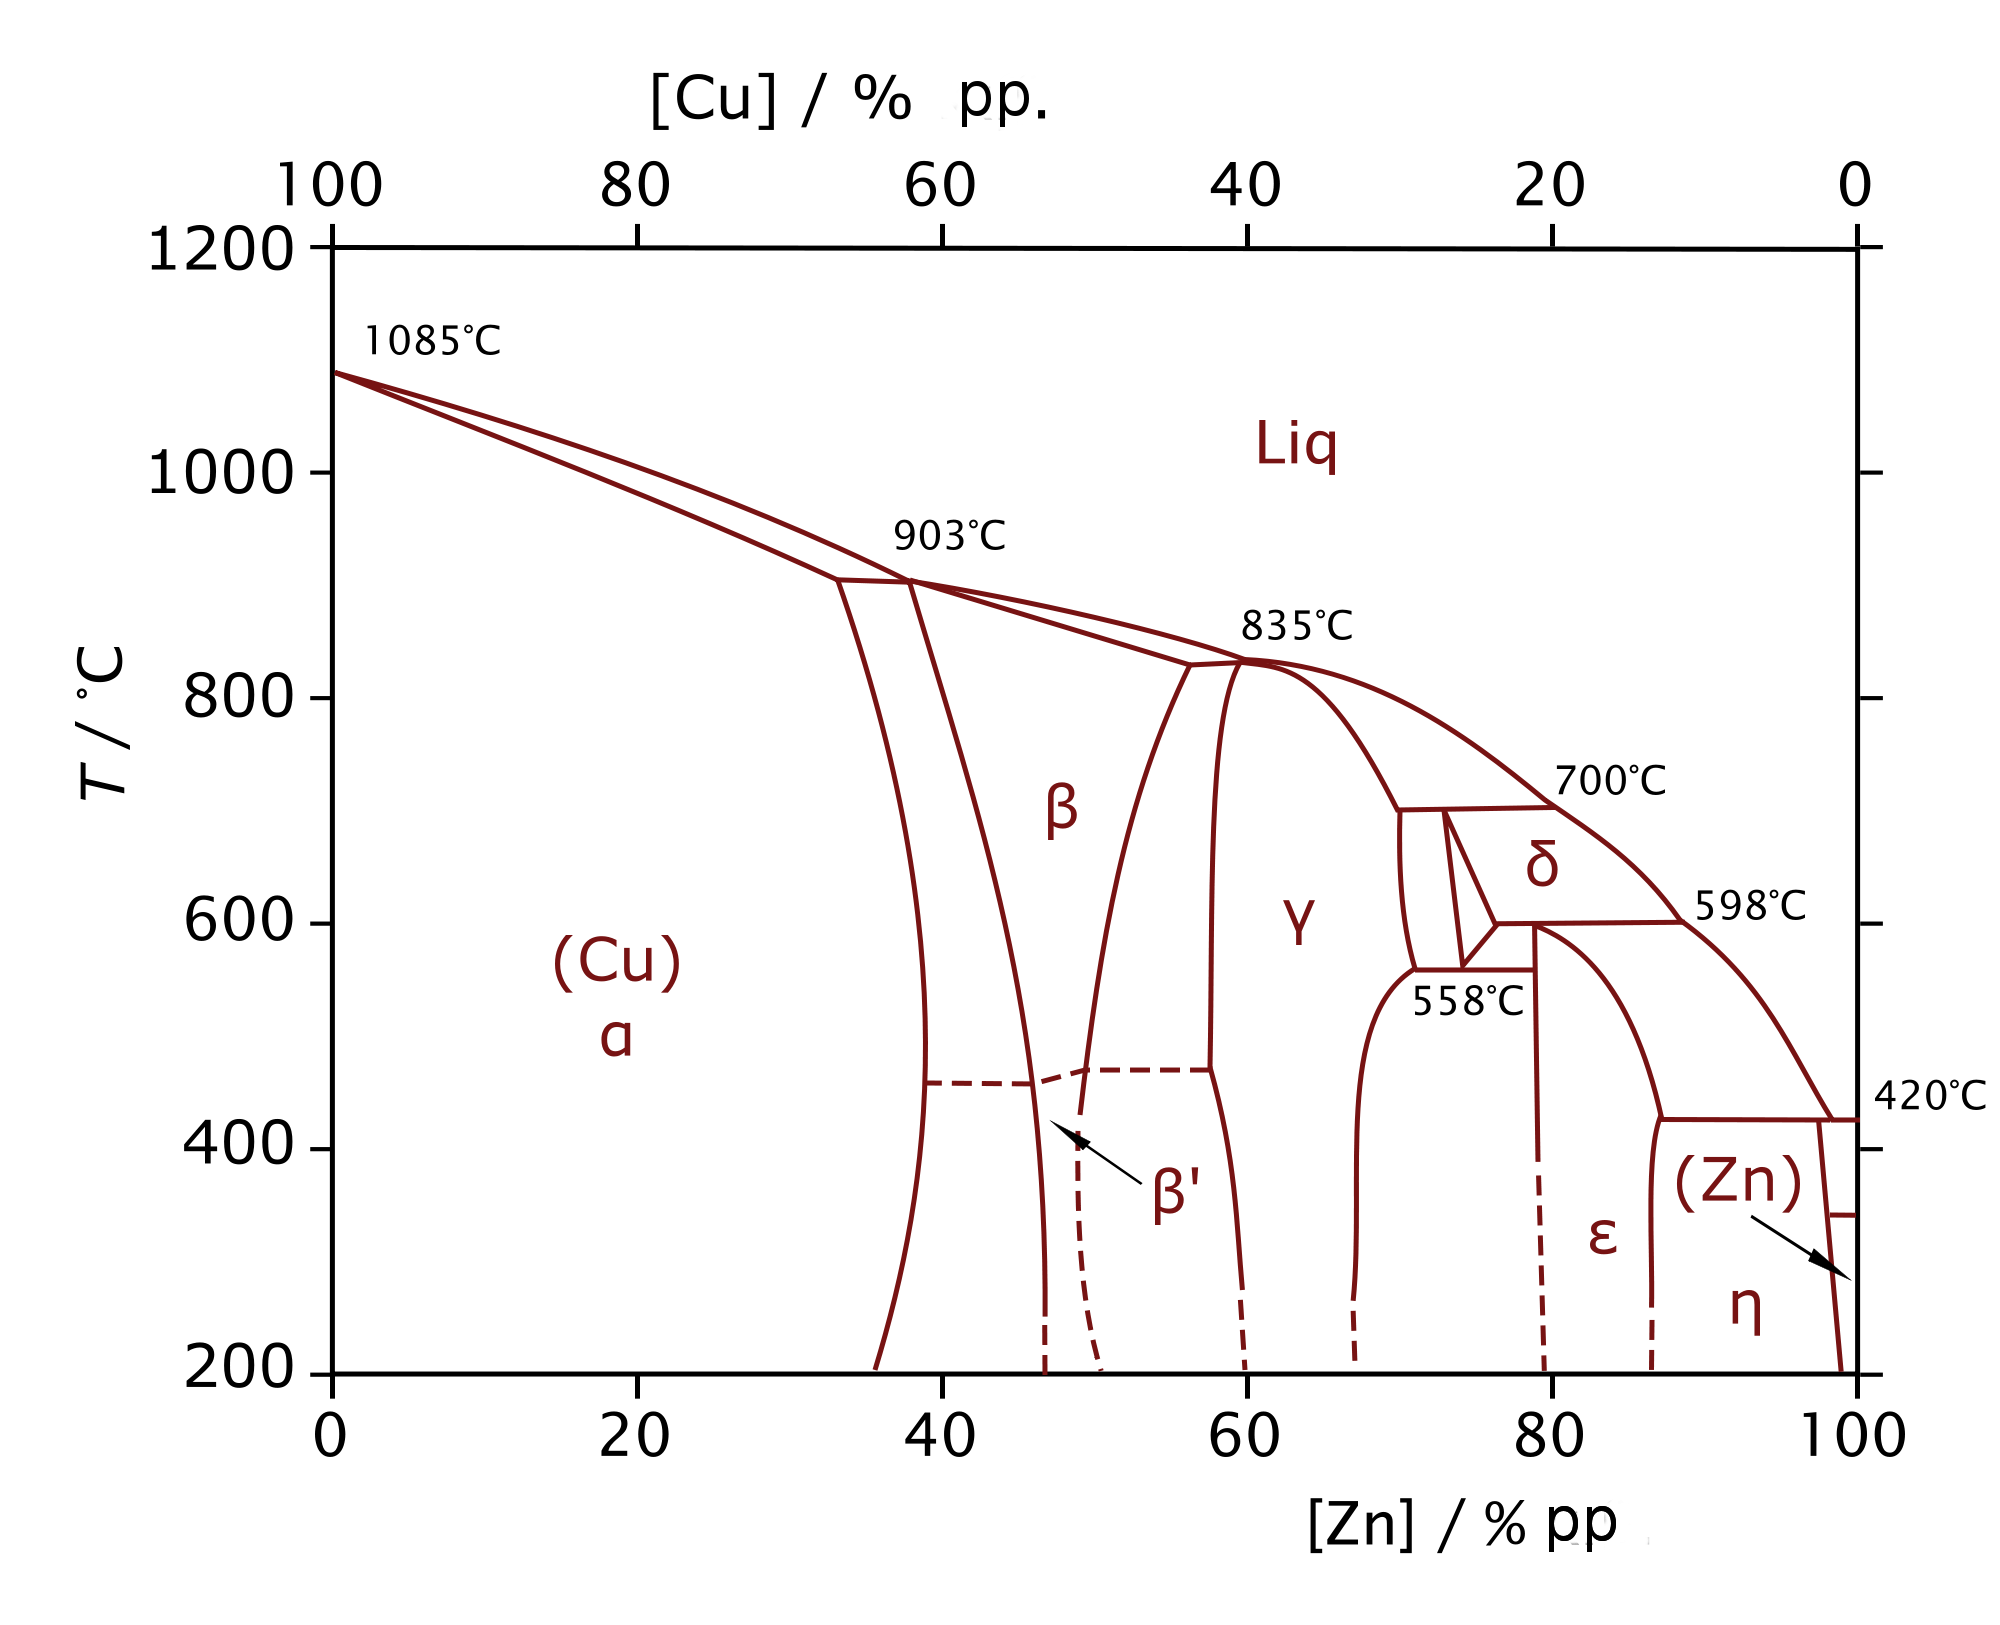
\includegraphics[width=0.6\textwidth]{img/intro/CuZn.png} 
% \end{center}
% \end{frame}

 
% \begin{equation*}
%  \beta \rightarrow B2 \rightarrow L2_1 \rightarrow 18R 
% \end{equation*}
%%%%%%%%%%%%%%%%%%%%%%%%%%%%%%%%%%%%%%%%%%%%%%%%%%%%%%%%%%%%%%%%%%%%%%%%%%%%%%%%%%%%%%%%%%%%%%%%%%%%%%%%%%%%%%%%
\begin{frame}

\frametitle{Aleación Cu-Zn-Al}

% \begin{figure}
% \begin{tikzpicture}
% 
% \draw[green, very thick, dashed] (-1.5,-0.5) -- (-1.5,4);
% 
% % 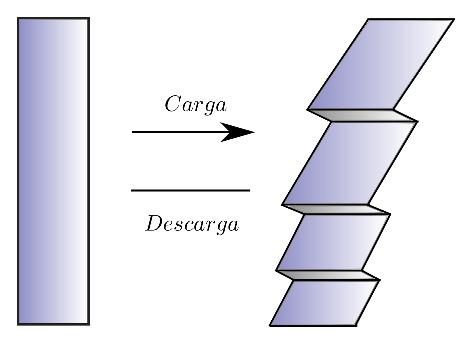
\includegraphics[width=0.4\columnwidth]{img/intro/HisteresisEsquema.eps}
% \node[anchor=south west,inner sep=0] (image) at (-5.5,-1) {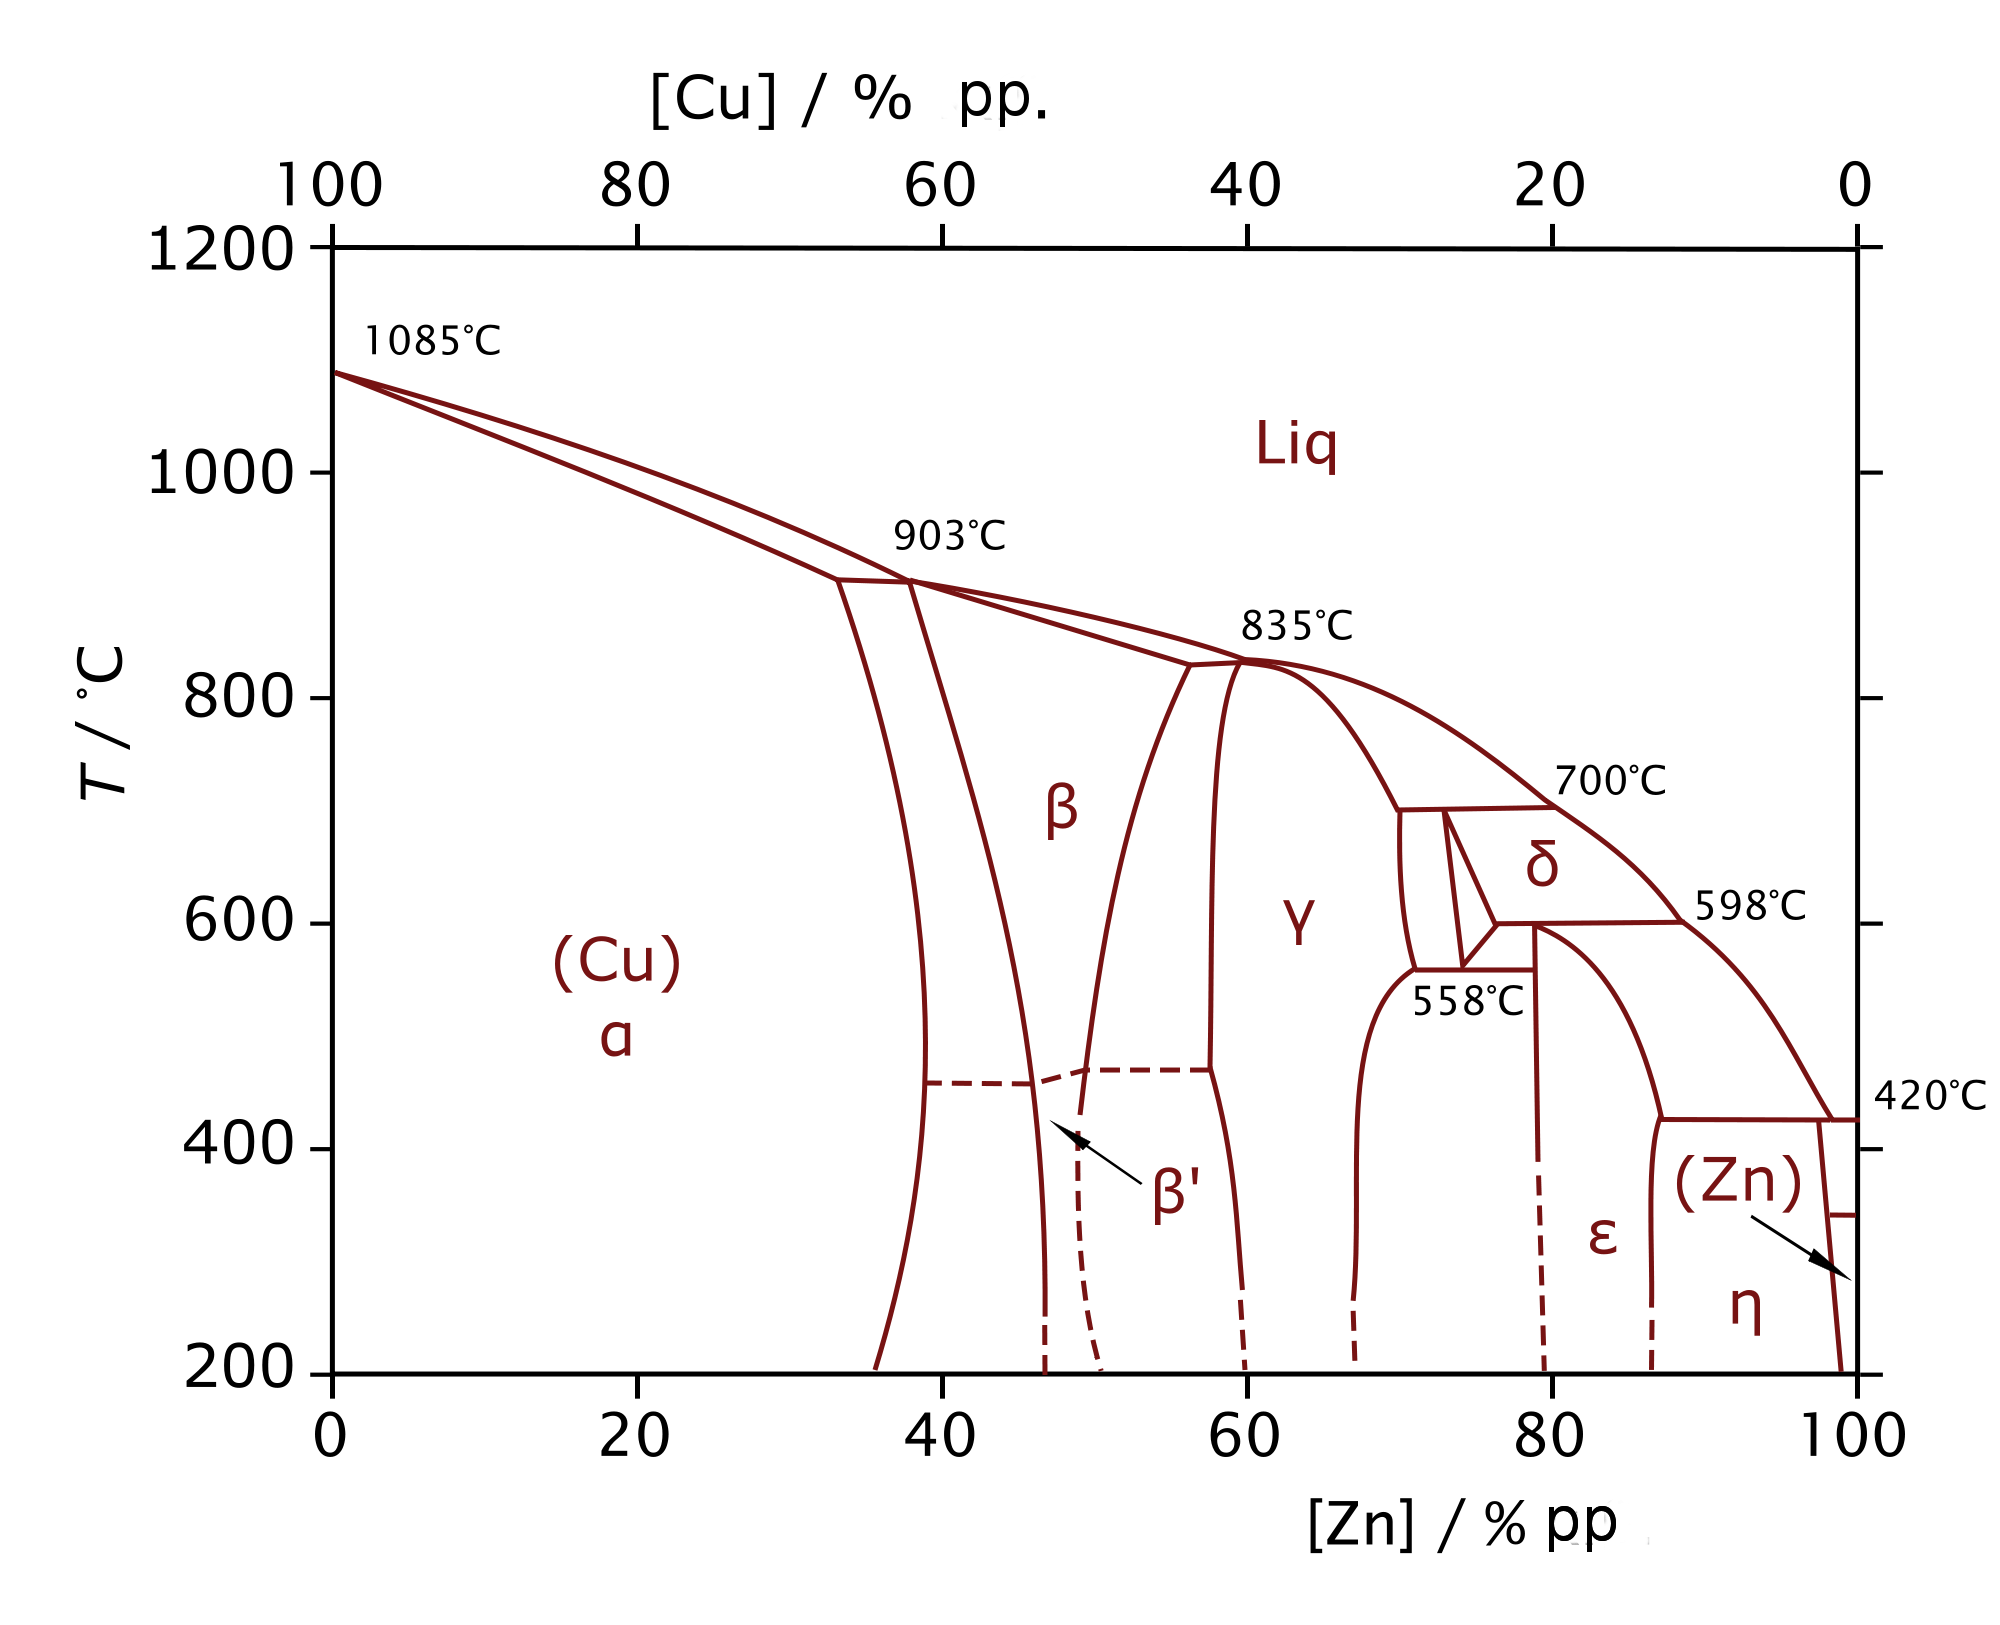
\includegraphics[width=0.7\textwidth]{img/intro/CuZn.png}};
% \node[anchor=south west,inner sep=0] (image) at (-2.5,-1.5) {$\frac{e}{a}=1.48$};
%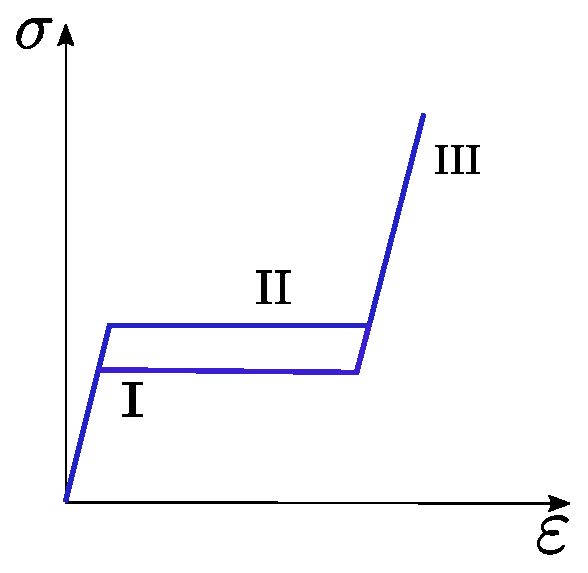
\includegraphics[width=0.4\columnwidth]{img/intro/Histeresis.eps}

% \pgftext{%
%  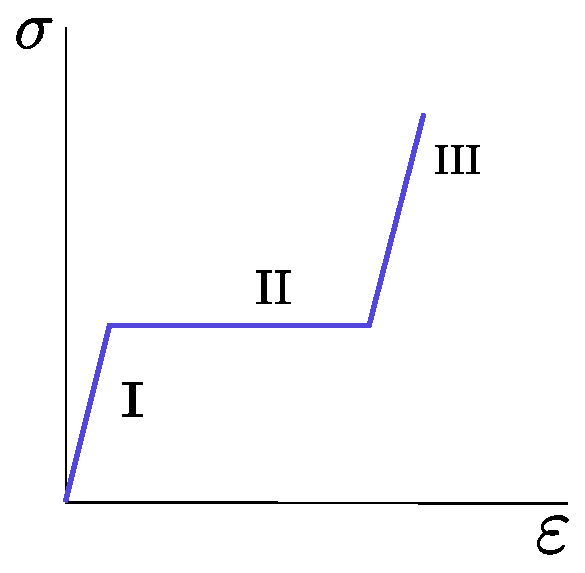
\includegraphics[width=0.4\textwidth]{img/intro/SigmavsDef.eps}
% }%

\begin{columns}

\column{0.5\textwidth}
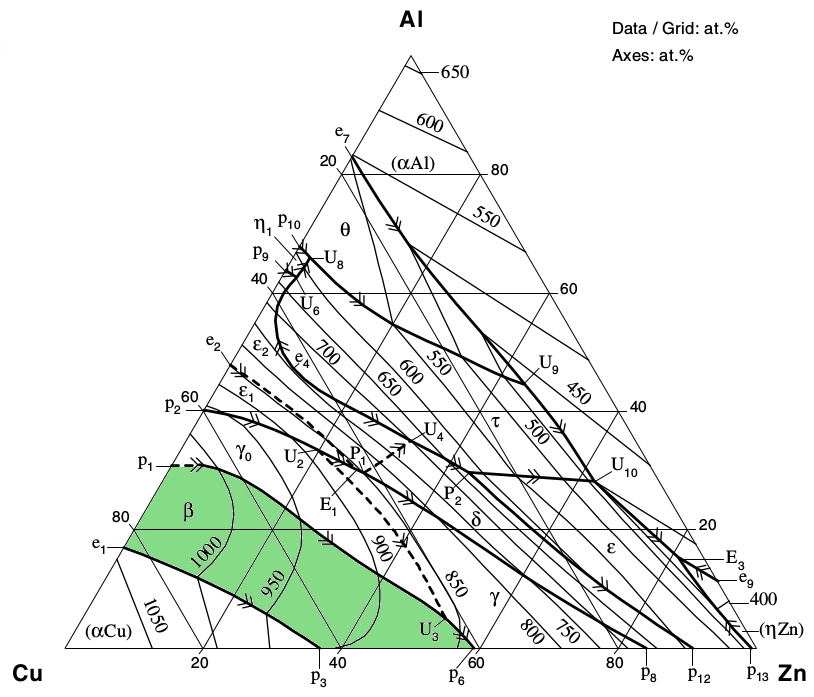
\includegraphics[width=\columnwidth]{img/intro/IsotermaLiq.png}
\column{0.5\textwidth}
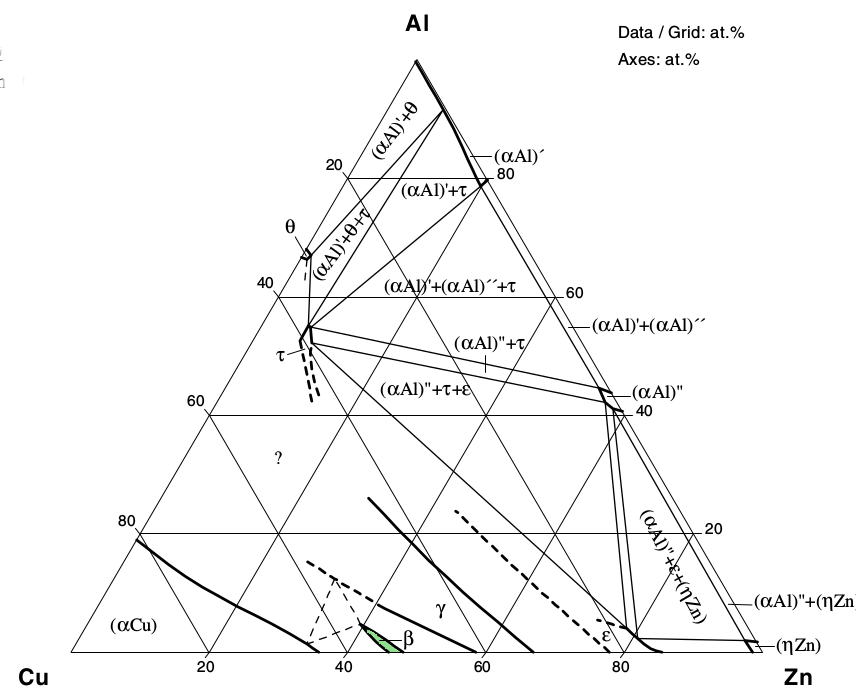
\includegraphics[width=\columnwidth]{img/intro/Isoterma300.png}

\end{columns}

\begin{center}
\begin{columns}
  \column{0.02\textwidth}
  
 \column{0.18\textwidth}
 Liquidus
 \column{0.05\textwidth}
 
  \column{0.2\textwidth}
 $300$ $^\circ C$
 \end{columns}
\end{center}

\end{frame}



% %%%%%%%%%%%%%%%%%%%%%%%%%%%%%%%%%%%%%%%%%%%%%%%%%%%%%%%%%%%%%%%%%%%%%%%%%%%%%%%%%%%%%%%%%%%%%%%%%%%%%%%%%%%%%%%%%%%%%%%%%%%%%%%%%%%%%%%%%55

\begin{frame}

\frametitle{Concentración electrónica}

\begin{columns}
\column{0.4\textwidth}
\begin{block}{
Concentración electrónica:
}

\begin{small}
\begin{itemize}
 \item Ag, Au, Cu: 1
 \item Be, Cd, Zn: 2
 \item Al: 3
\end{itemize}
\end{small}
\end{block}
$\Longrightarrow$ Hume-Rothery


\begin{block}{Cu-Zn-Al
}
$\frac{e}{a} = 1+C_{Zn}+2C_{Al}$

Usamos $e/a=1.48$
\end{block}
%     \begin{tiny}
%     \begin{itemize}
%  \item $Cu=75,20$ $\%pp$
%   \item $Zn=17,14$ $\%pp$
%   \item $Al=7,66$ $\%pp$
%  \end{itemize}
% \end{tiny} 
  
\column{0.6\textwidth}
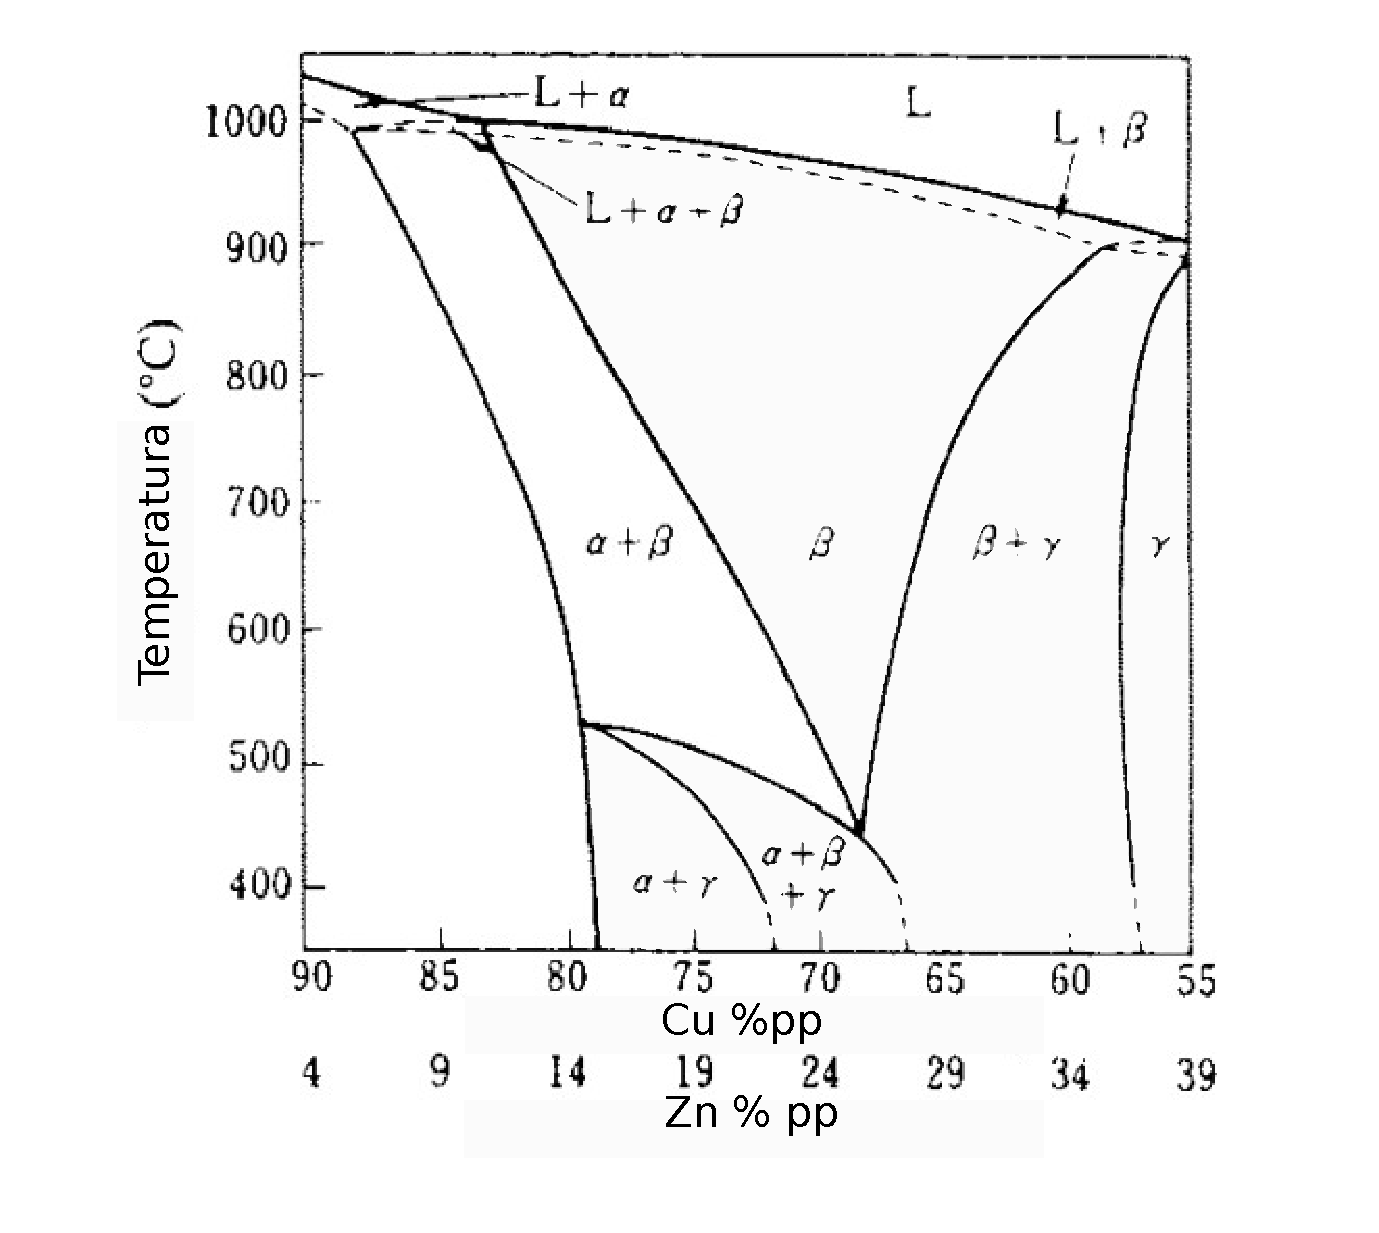
\includegraphics[width=\columnwidth]{img/intro/CuZnAl.eps}
\begin{center}
\begin{small}
\quad $Al=6$ $\% pp$
\end{small}
\end{center}
\end{columns}
\end{frame}

%%%%%%%%%%%%%%%%%%%%%%%%%%%%%%%%%%%%%%%%%%%%%%%%%%%%%%%%%%%%%%%%%%%%%%%%%%%%%%%%%%%%%%%%%%%%%%%%%%%%%%%%%%%%%%%%%%%%%%%%%%%%

\begin{frame}

\frametitle{Temperatura de transición martensítica ($M_s$)}

\begin{columns}
\column{0.5\textwidth}
\begin{block}{
Concentración electrónica:
}\begin{equation*}
\frac{e}{a} = 1+C_{Zn}+2C_{Al}
\end{equation*}
\end{block}
\begin{block}{
Ecuación empírica para $M_s$
} \begin{equation*}
M_s[K]=2686-6400C_{Zn}-9000C_{Al} \label{Ms} 
\end{equation*}
\end{block}
\begin{block}{
Composiciones:
}\begin{equation*}
     C_{Cu}+C_{Zn}+C_{Al}=1
\end{equation*}
\end{block}
\column{0.6\textwidth}
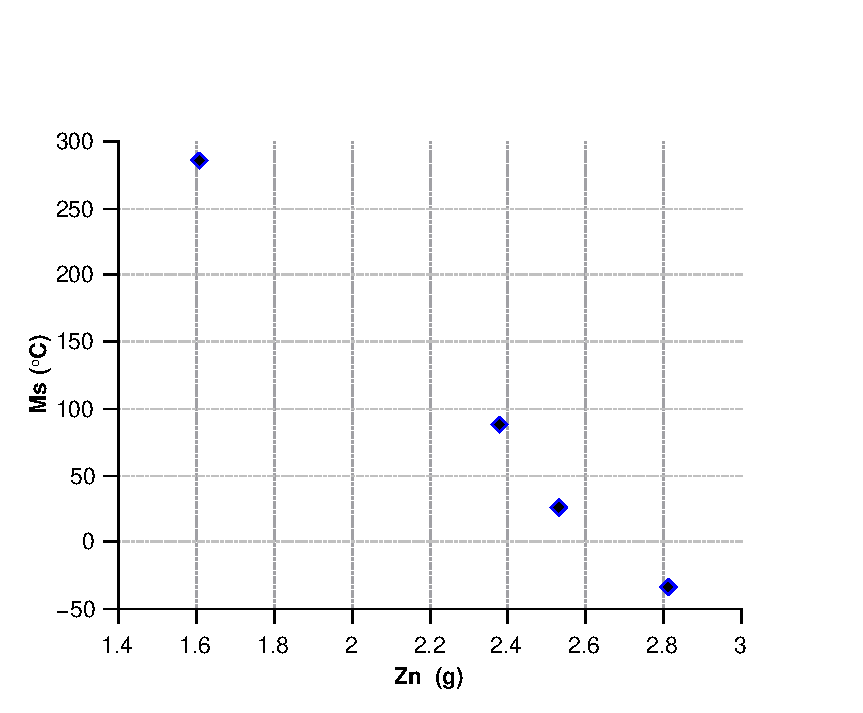
\includegraphics[width=\columnwidth]{img/intro/MsZn2.eps}
\begin{tiny}
\begin{itemize}
 \item Cu= $12,53$ g
 \item Al= $1,28$ g
\end{itemize}
\end{tiny}

\end{columns}
\end{frame}

% \begin{figure}
% \begin{tikzpicture}
% \node[align=left] (It)   at (0, 0)[rectangle, draw, red] {Explicar relación entre fórmulas y la $M_s$ buscada};
% \end{tikzpicture}
% \end{figure}







%%%%%%%%%%%%%%%%%%%%%%%%%%%%%%%%%%%%%%%%%%%%%%%%%%%%%%%%%%%%%%%%%%%%%%%%%%%%%%%%%%%%%%%%%%%%%%%%%%%%%%%%%%%%%%%%
\begin{frame}
 \frametitle{Estructuras celulares}

 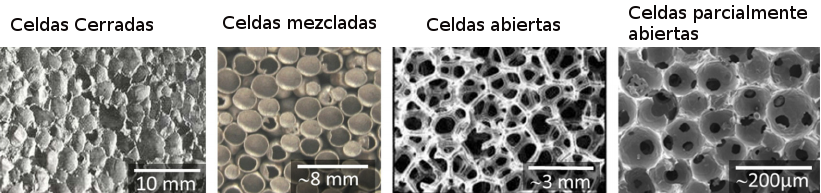
\includegraphics[width=\columnwidth]{img/intro/Fig-1-The-different-kinds-of-cellular-solids-from-closed-cells-to-open-cells.png}
\vfill 
 
 \begin{columns}
 \column{0.4\textwidth}
 % Prototipo de cabinas de tren
 Cabina de tren
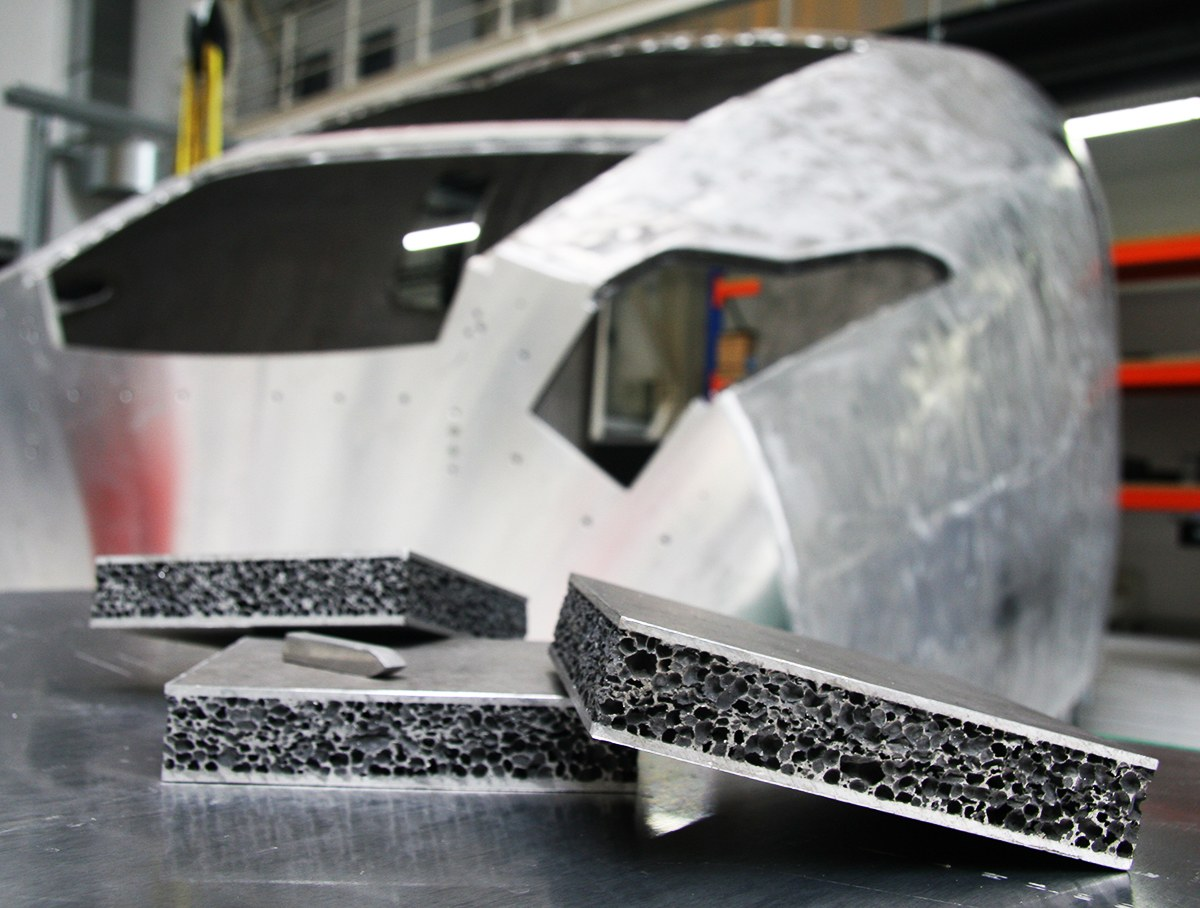
\includegraphics[width=0.8\columnwidth]{img/intro/aluminum-foam-ft.jpg}
% \column{0.33\textwidth}
% 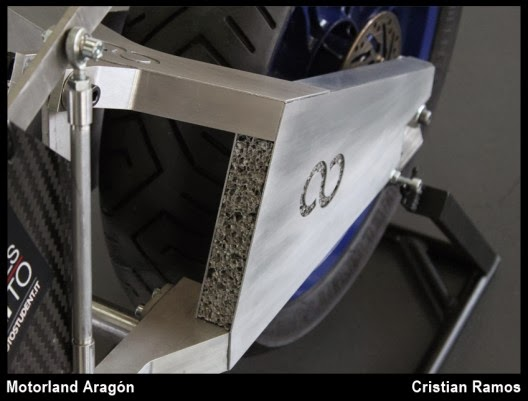
\includegraphics[width=0.8\columnwidth]{img/intro/DSC125_Motorland2-528x401.jpg}
\column{0.4\textwidth}
Honeycomb
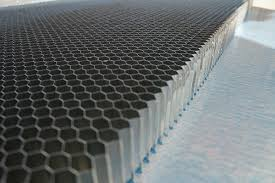
\includegraphics[width=0.8\columnwidth]{img/intro/honneycomb.jpeg}
\end{columns}

\end{frame}




%%%%%%%%%%%%%%%%%%%%%%%%%%%%%%%%%%%%%%%%%%%%%%%%%%%%%%%%%%%%%%%%%%%%%%%%%%%%%%%%%%%%%%%%%%%%%%%%%%%%%%%%%%%%%%%%

\begin{frame}
\frametitle{Esponjas metálicas}
% \begin{tiny}
% Esponja elastoplástica de Cu: Densidad relativa $0,17$ y celdas de $3$ $mm$
% \end{tiny}
\begin{figure}
\begin{tikzpicture}
% \pgftext{%
%  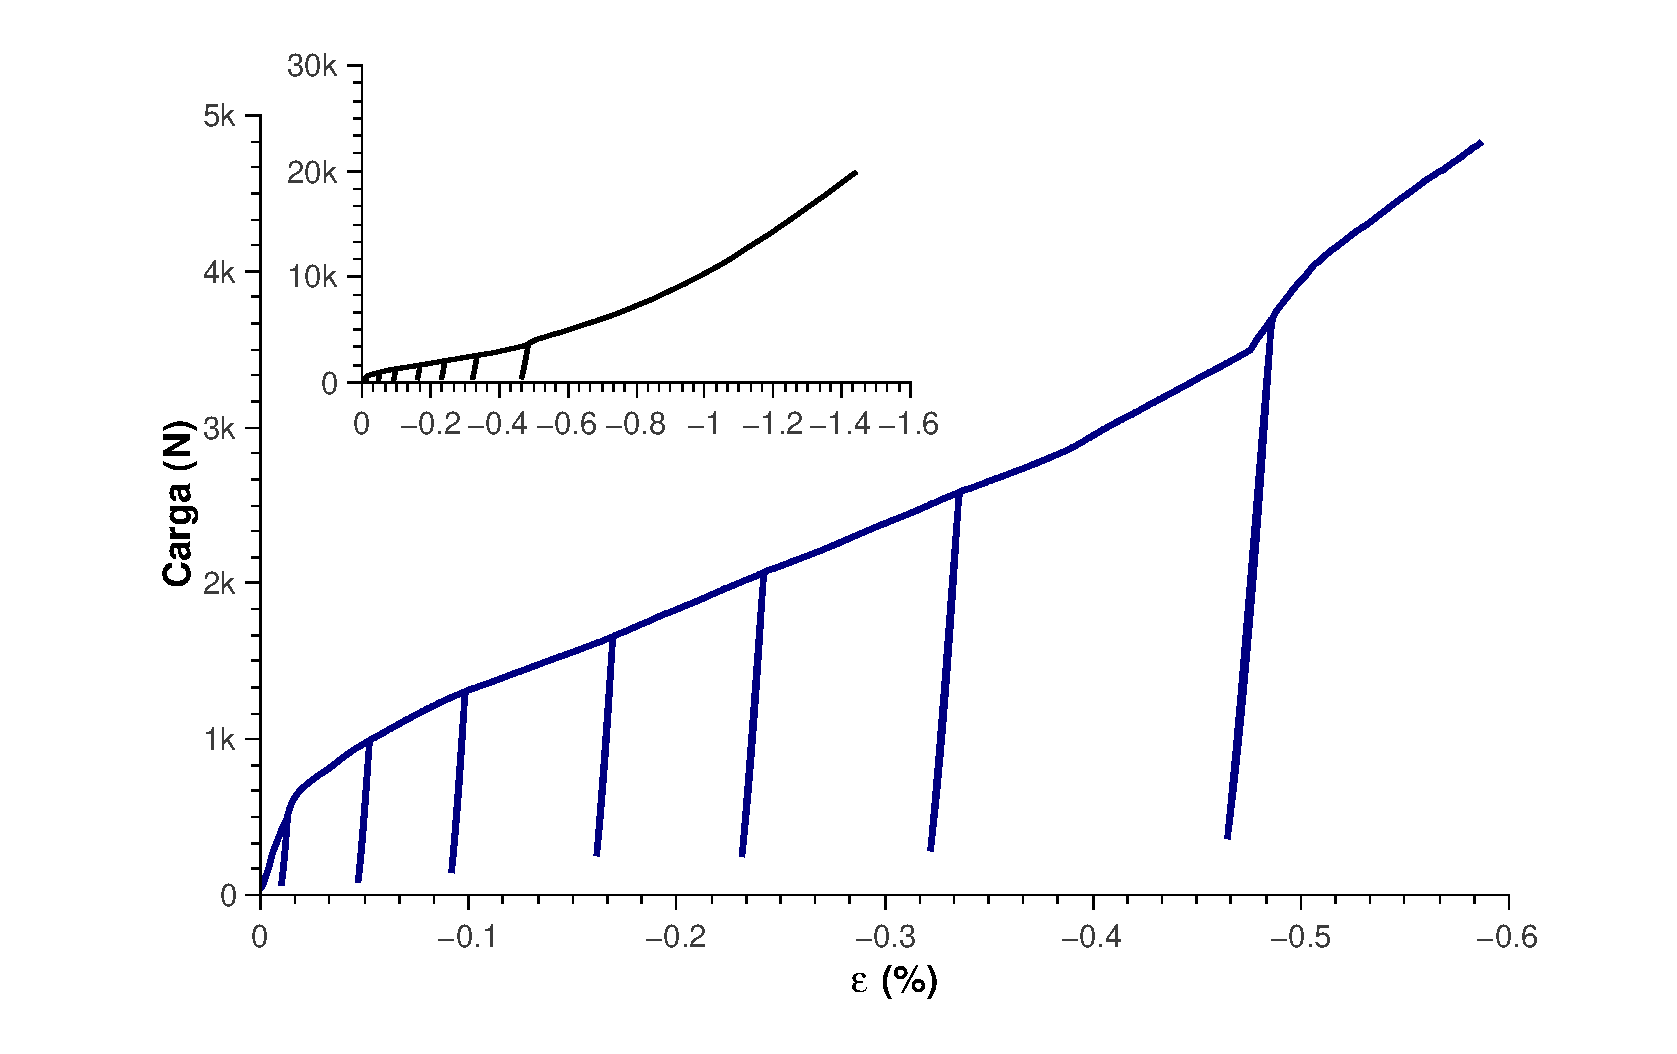
\includegraphics[width=0.8\textwidth]{img/intro/Cucompararesponja.eps}
% }%
\node[anchor=south west,inner sep=0] (image) at (-5,-2) {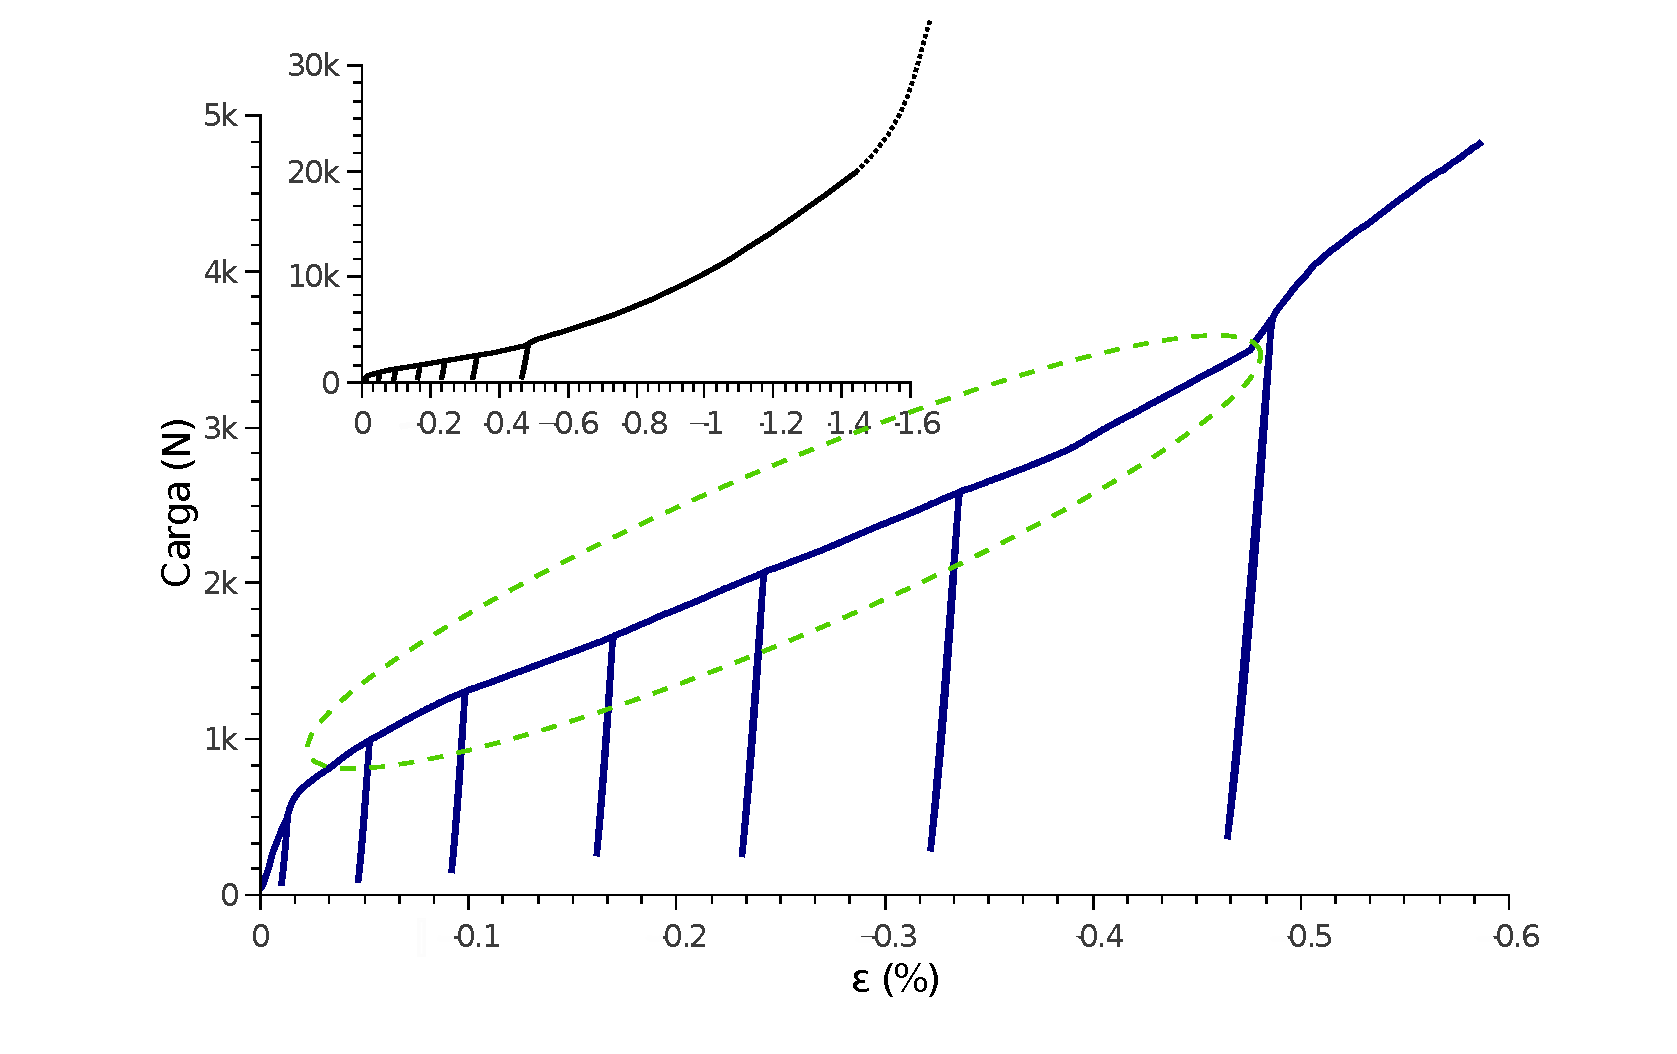
\includegraphics[width=0.8\textwidth]{img/intro/Cucompararesponja3.eps}};
\node (I) at (-3.6,-0.9) {};
\node (II) at (-0.1, 0.5) {};
\node (III) at (-0.2, 3) {};
\node[align=left] (It)   at (0.1,-2.5) {Lineal-elástico $\rightarrow$ flexión de las paredes };
\node[align=left] (IIt)  at (5,0) {Deformación o \\ fractura localizada};
\node[align=left] (IIIt) at (1, 4) {Compactación};
% \draw[green, dashed, thick] (-1,0.5) ellipse  (3cm and 0.5cm);
% 
\path[->]<1-> (I) edge [green, dashed,  thick] (It);
\path[->]<1-> (II) edge [green, dashed,  thick] (IIt);
\path[->]<1-> (III) edge [green, dashed, thick] (IIIt);

%\node[align=left] (It)   at (0, 0)[rectangle, draw, red] {Carga y deformación +};

\end{tikzpicture}
\end{figure}

\end{frame}
% 
% 
% 
% 
% \begin{multicols}{2}
% 
% 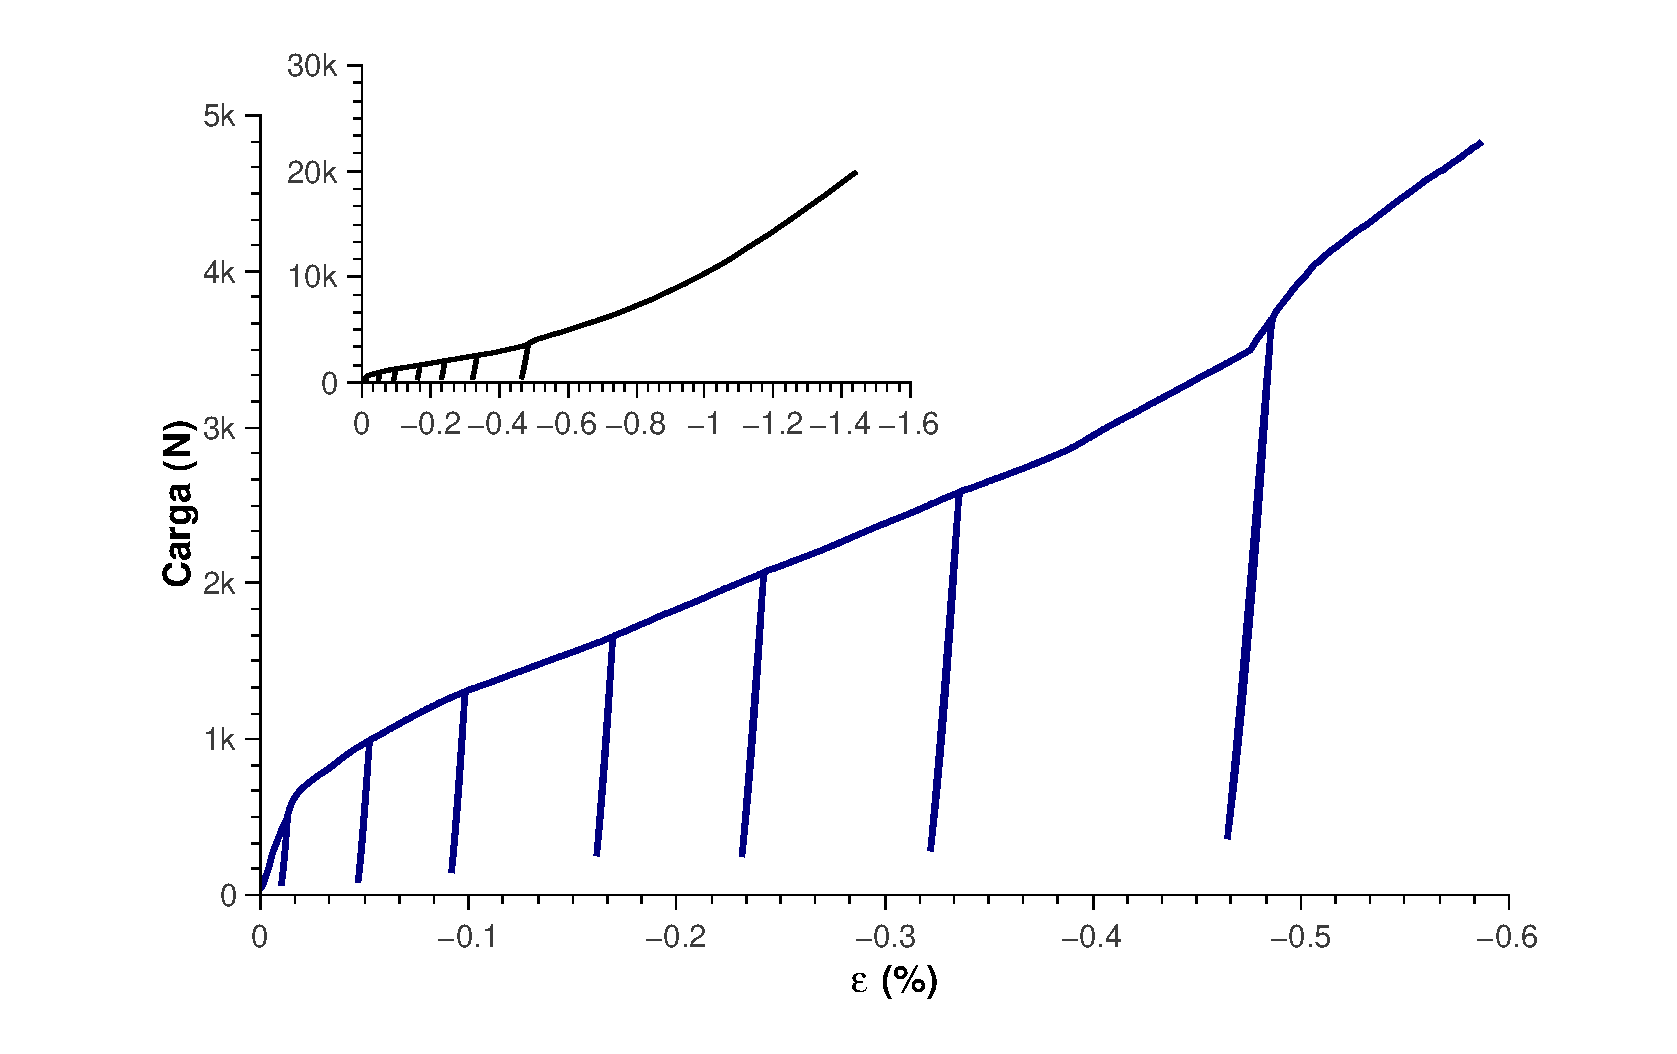
\includegraphics[width=0.5\textwidth]{img/intro/Cucompararesponja.eps}
% 
% \begin{itemize}
% \small
%  \item \alert<1>{Lineal-elástico $\rightarrow$ flexión de las paredes }
%  \item \alert<2>{Colapso de la estructura $\rightarrow$ Fluencia o fractura}
%  \item \alert<3>{Densificación  }
% \end{itemize}
% 
% \end{multicols}
% \alert<4>{Principal parámetro: Densidad específica $\frac{\rho^*}{\rho_s}$}
% 
% Principal forma de caracterizar las propiedades mecánicas 
% \alert<5>{
% \begin{equation*}
% \frac{F^*}{F_s}=A \left(\frac{\rho^*}{\rho_s}\right)^n \label{props} 
% \end{equation*}
% }
% sirve para rigidez de la estructura, tensión de colapso de la estructura $\sigma^{pl}$,
% Deformación en bandas a $45 ^\circ$
% 


%%%%% Lo saco pq no lo usamos
% \begin{frame}
% \frametitle{Esponjas metálicas}
% 
% EXPLICAR MEJOR ESTAS FÓRMULAS
% 
% Principal parámetro: Densidad específica $\frac{\rho^*}{\rho_s}$
% 
% Principal forma de caracterizar las propiedades mecánicas 
% 
% \begin{equation*}
% \frac{F^*}{F_s}=A \left(\frac{\rho^*}{\rho_s}\right)^n \label{props} 
% \end{equation*}
% 
% sirve para rigidez de la estructura, tensión de colapso de la estructura $\sigma^{pl}$,y muchas otras propiedades mecánicas.
% 
% 
% \end{frame}


%%%%%%%%%%%%%%%%%%%%%%%%%%%%%%%%%%%%%%%%%%%%%%%%%%%%%%%%%%%%%%%%%%%%%%%%%%%%%%%%%%%%%%%%%%%%%%%%%%%%%%%%%%%%%%%%%%%%%%%%%%%%%%%%%%%%%%%%%%%%
\begin{frame}

\frametitle{Esponjas Pseudoelásticas}
 
 \begin{columns}
\column{0.5\textwidth}
 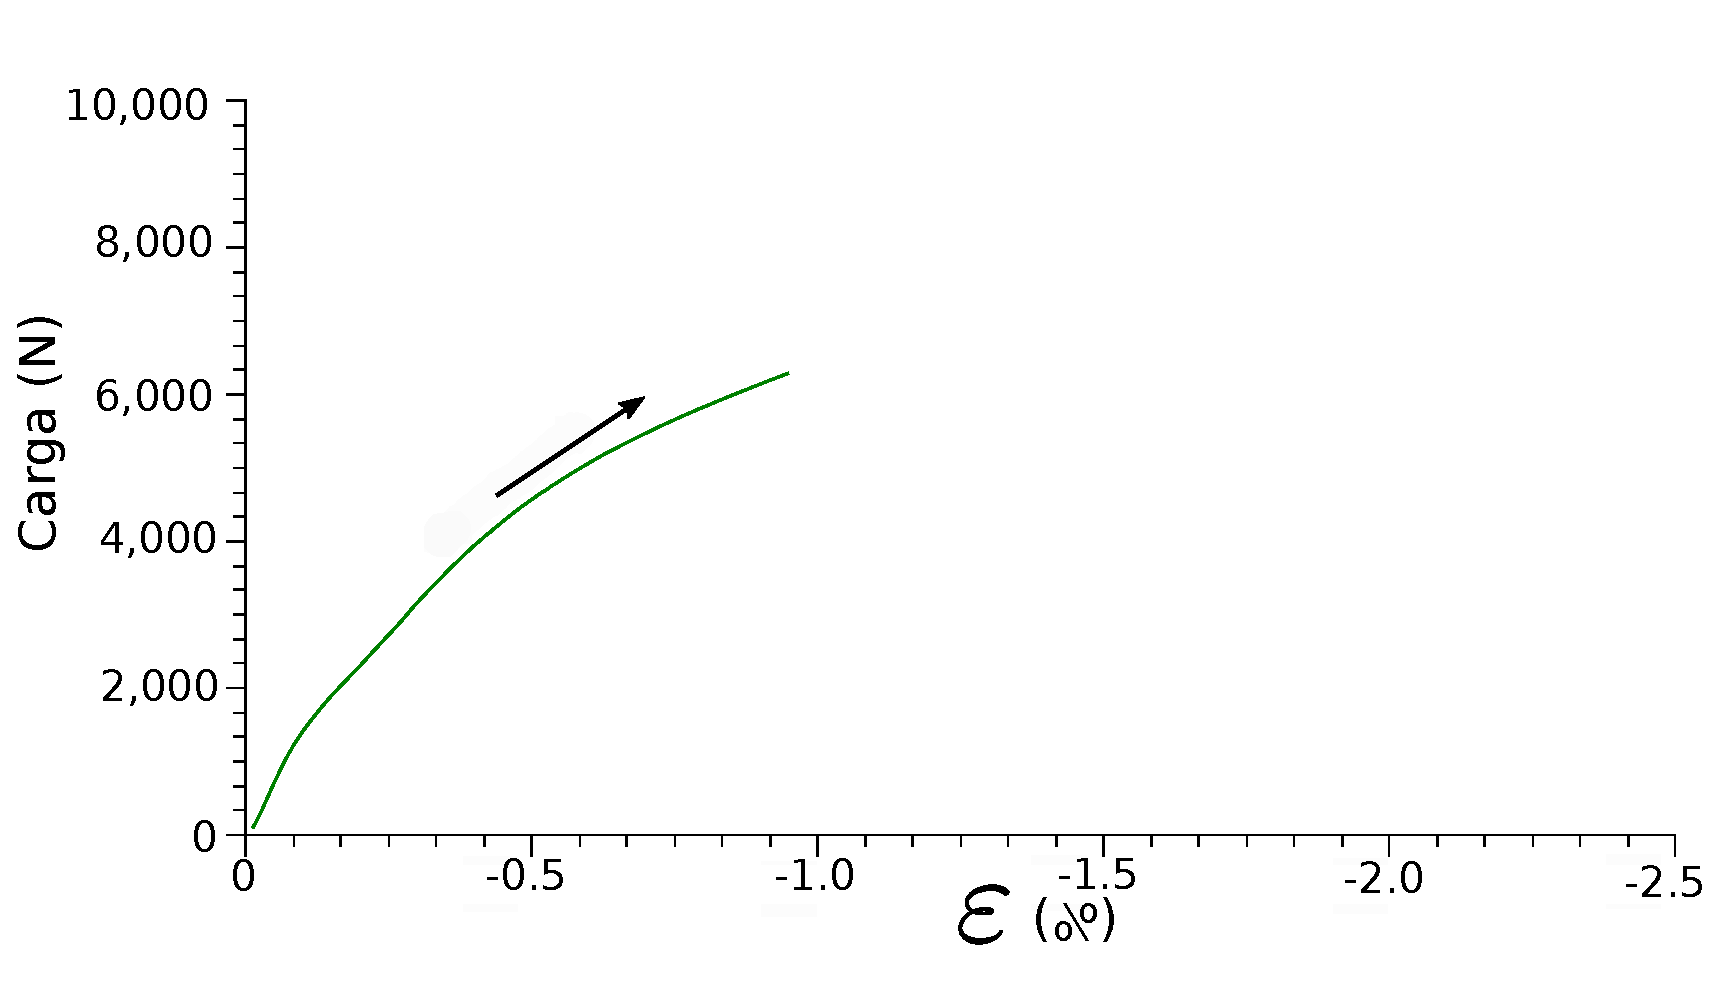
\includegraphics[width=\textwidth]{img/intro/Graph5111b.eps}
 
 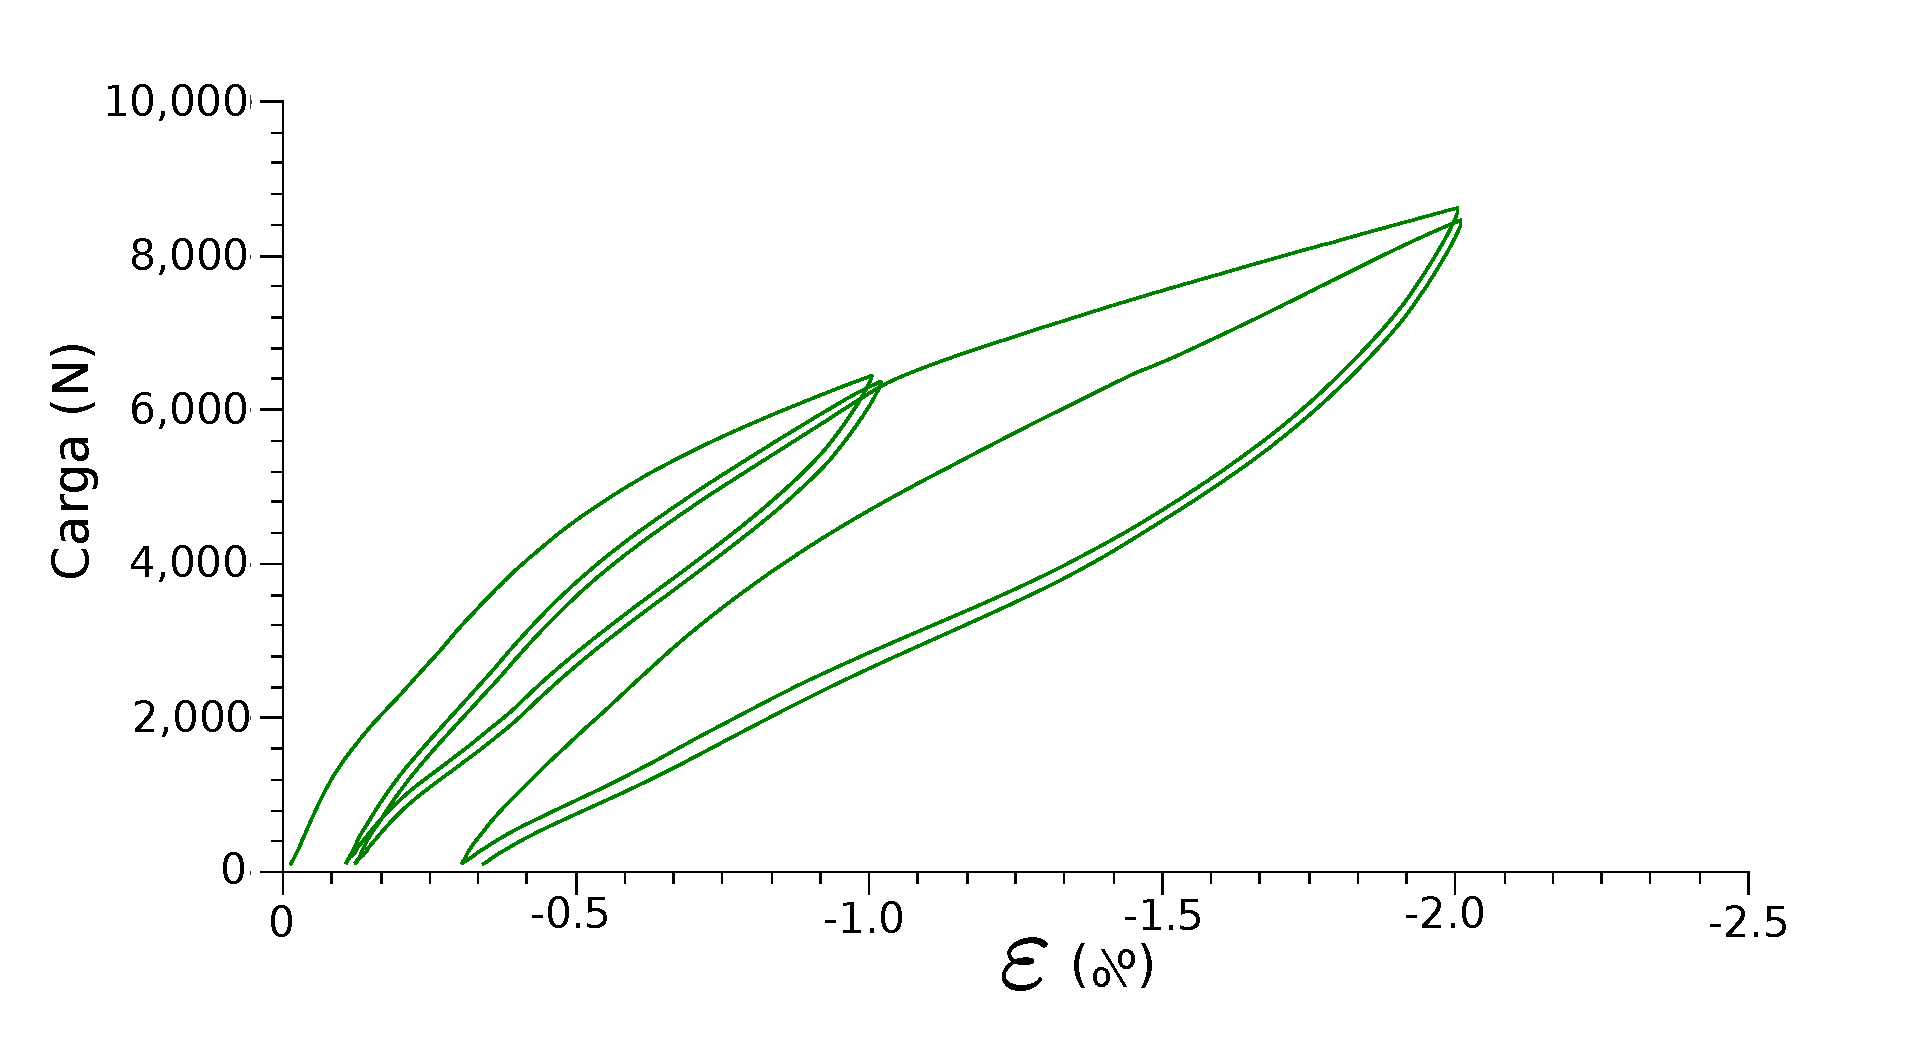
\includegraphics[width=\textwidth]{img/intro/Graph533b.eps}
 
\column{0.5\textwidth}
 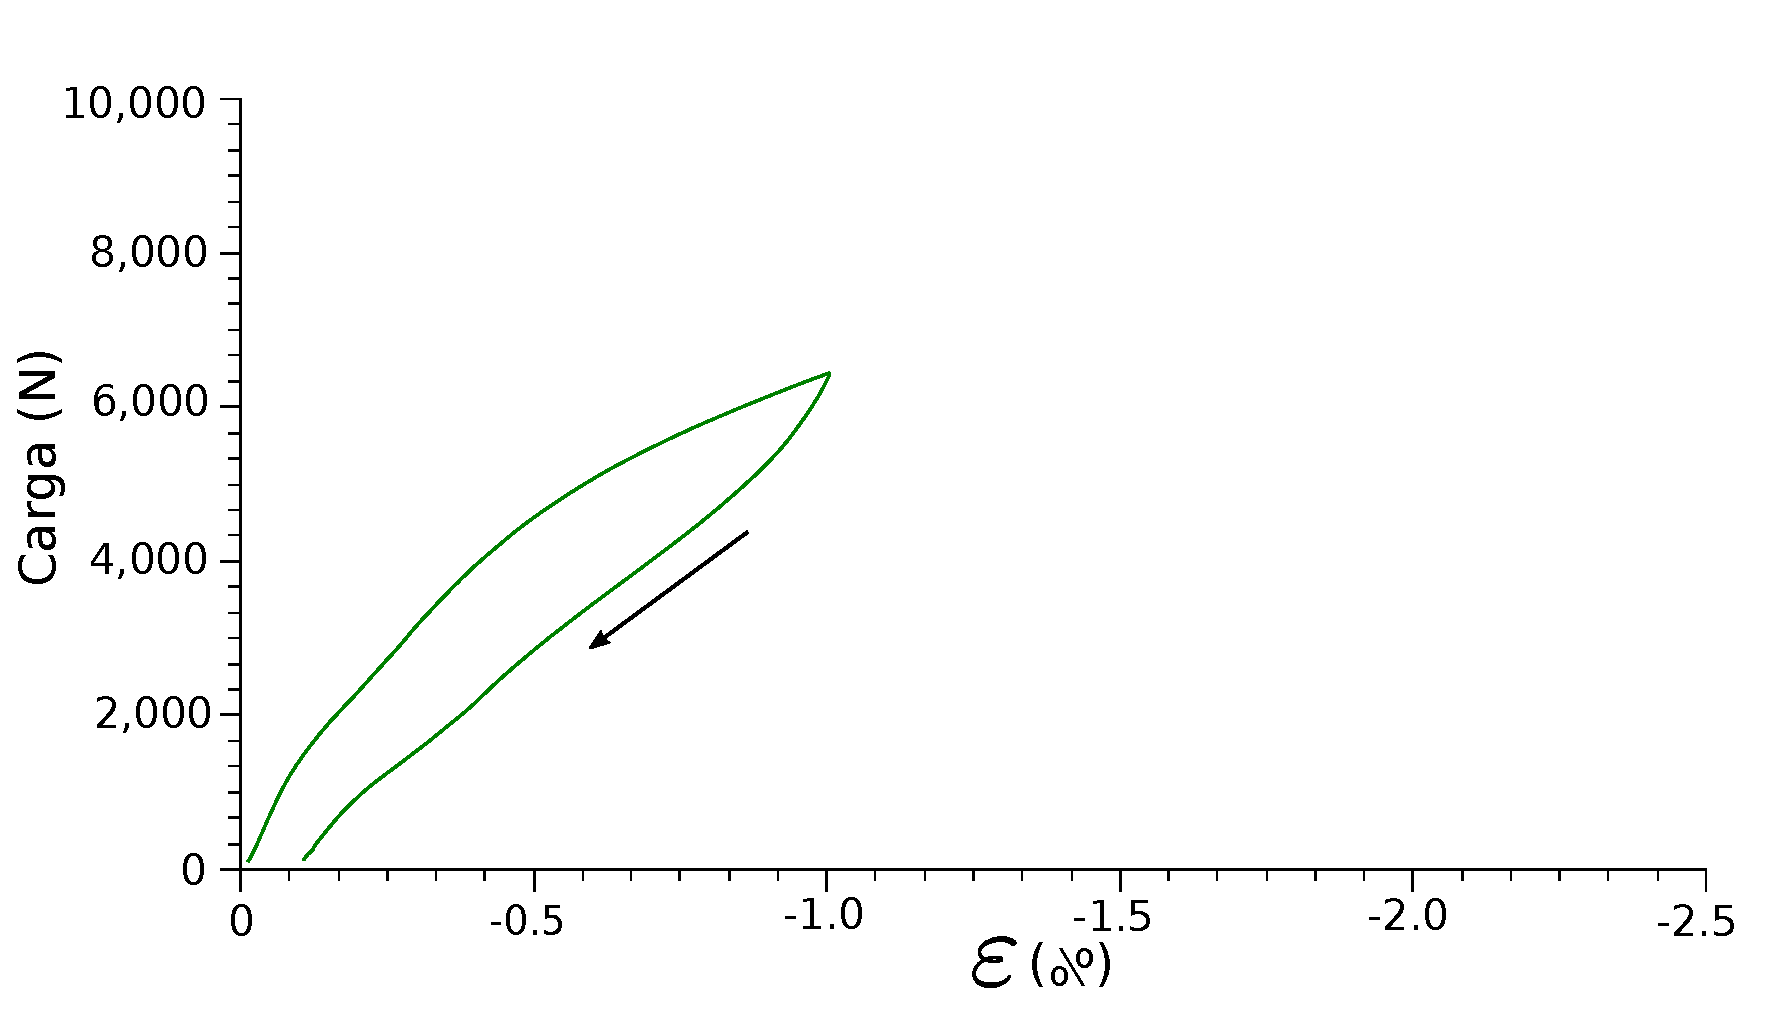
\includegraphics[width=\textwidth]{img/intro/Graph522b.eps}
  \begin{small}
\begin{itemize}
 \item Martensita retenida
 \item Deformación plástica
 \item Rotura de las paredes de las celdas
\end{itemize}
\end{small}
 \end{columns}
 \vspace{0.5 cm}
 \begin{small}
Esponja de Cu-Zn-Al de concentración electrónica 1,48, densidad específica $0,16$ y poros entre $1,4$ y $2,8$ $mm$.
\end{small}
\end{frame}


%%%%%%%%%%%%%%%%%%%%%%%%%%%%%%%%%%%%%%%%%%%%%%%%%%%%%%%%%%%%%%%%%%%%%%%%%%%%%%%%%%%%%%%%%%%%%%%%%%%%%%%%%%%%%%%%

\begin{frame}

\frametitle{Esponjas pseudoelásticas}


%  \begin{columns}
% \column{0.5\textwidth}
% \begin{small}
% Esponja elastoplástica
% \end{small}
% 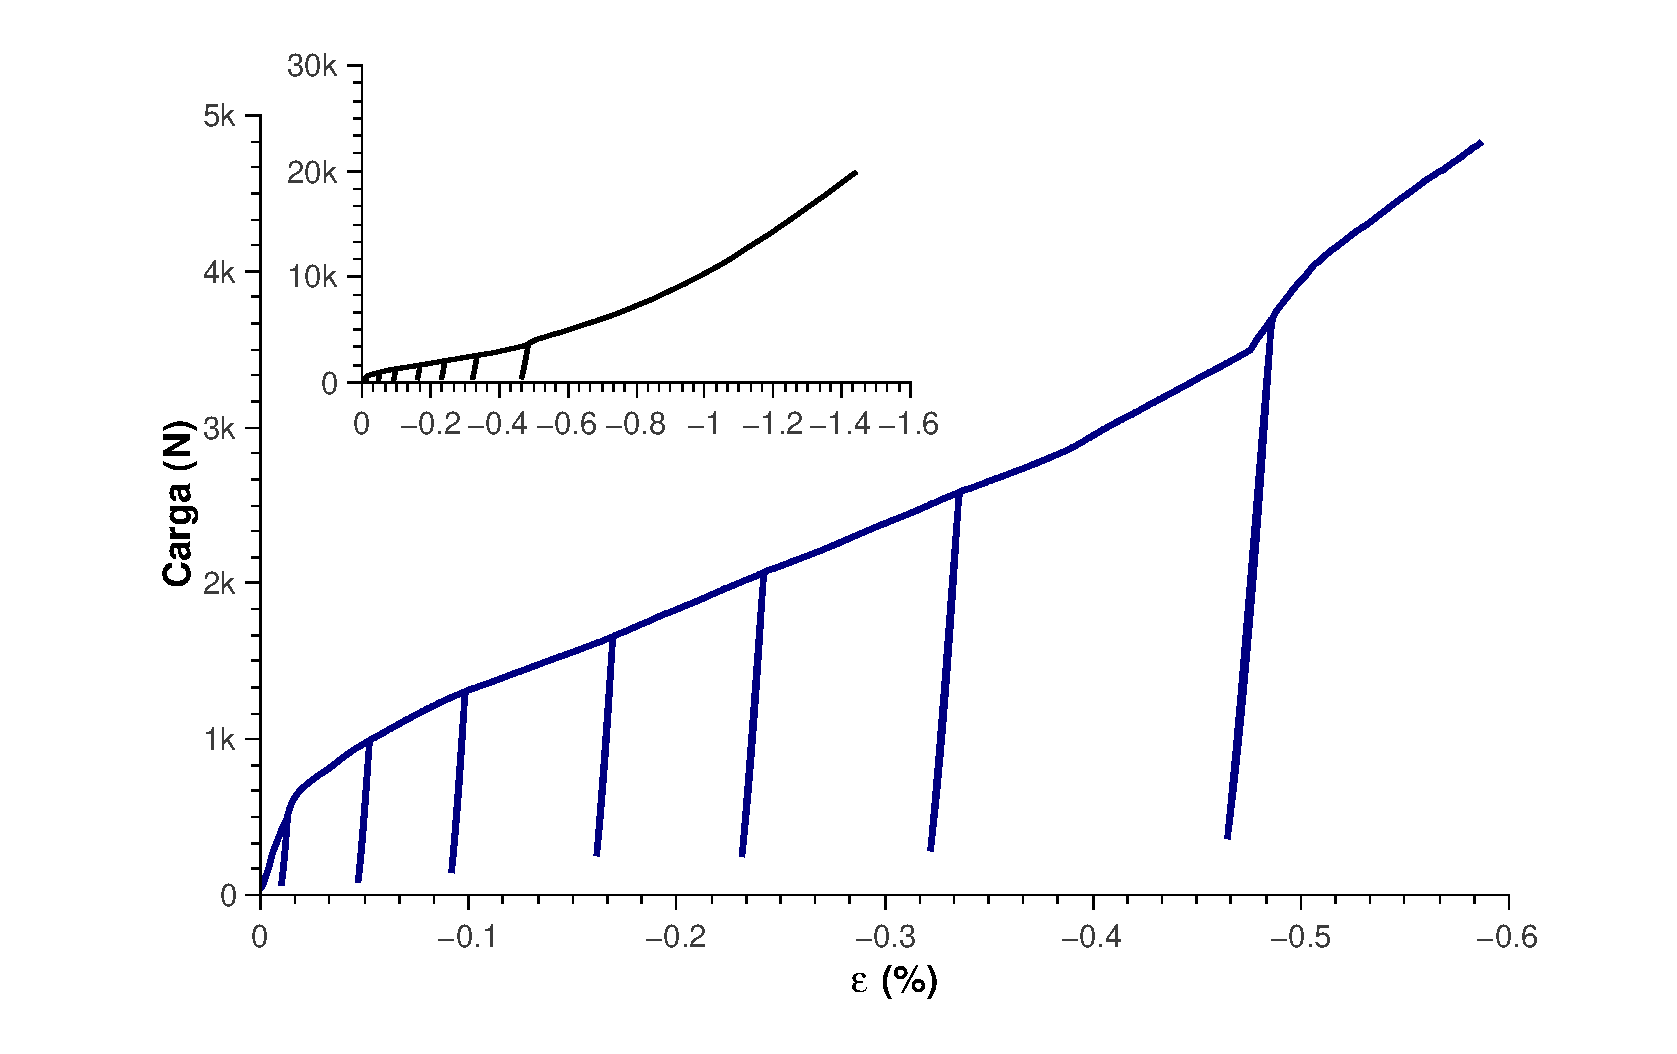
\includegraphics[width=0.9\columnwidth]{img/intro/Cucompararesponja.eps}
%  
% \column{0.6\textwidth} 
% \begin{small}
% Esponja pseudoelástica
% \end{small}
% 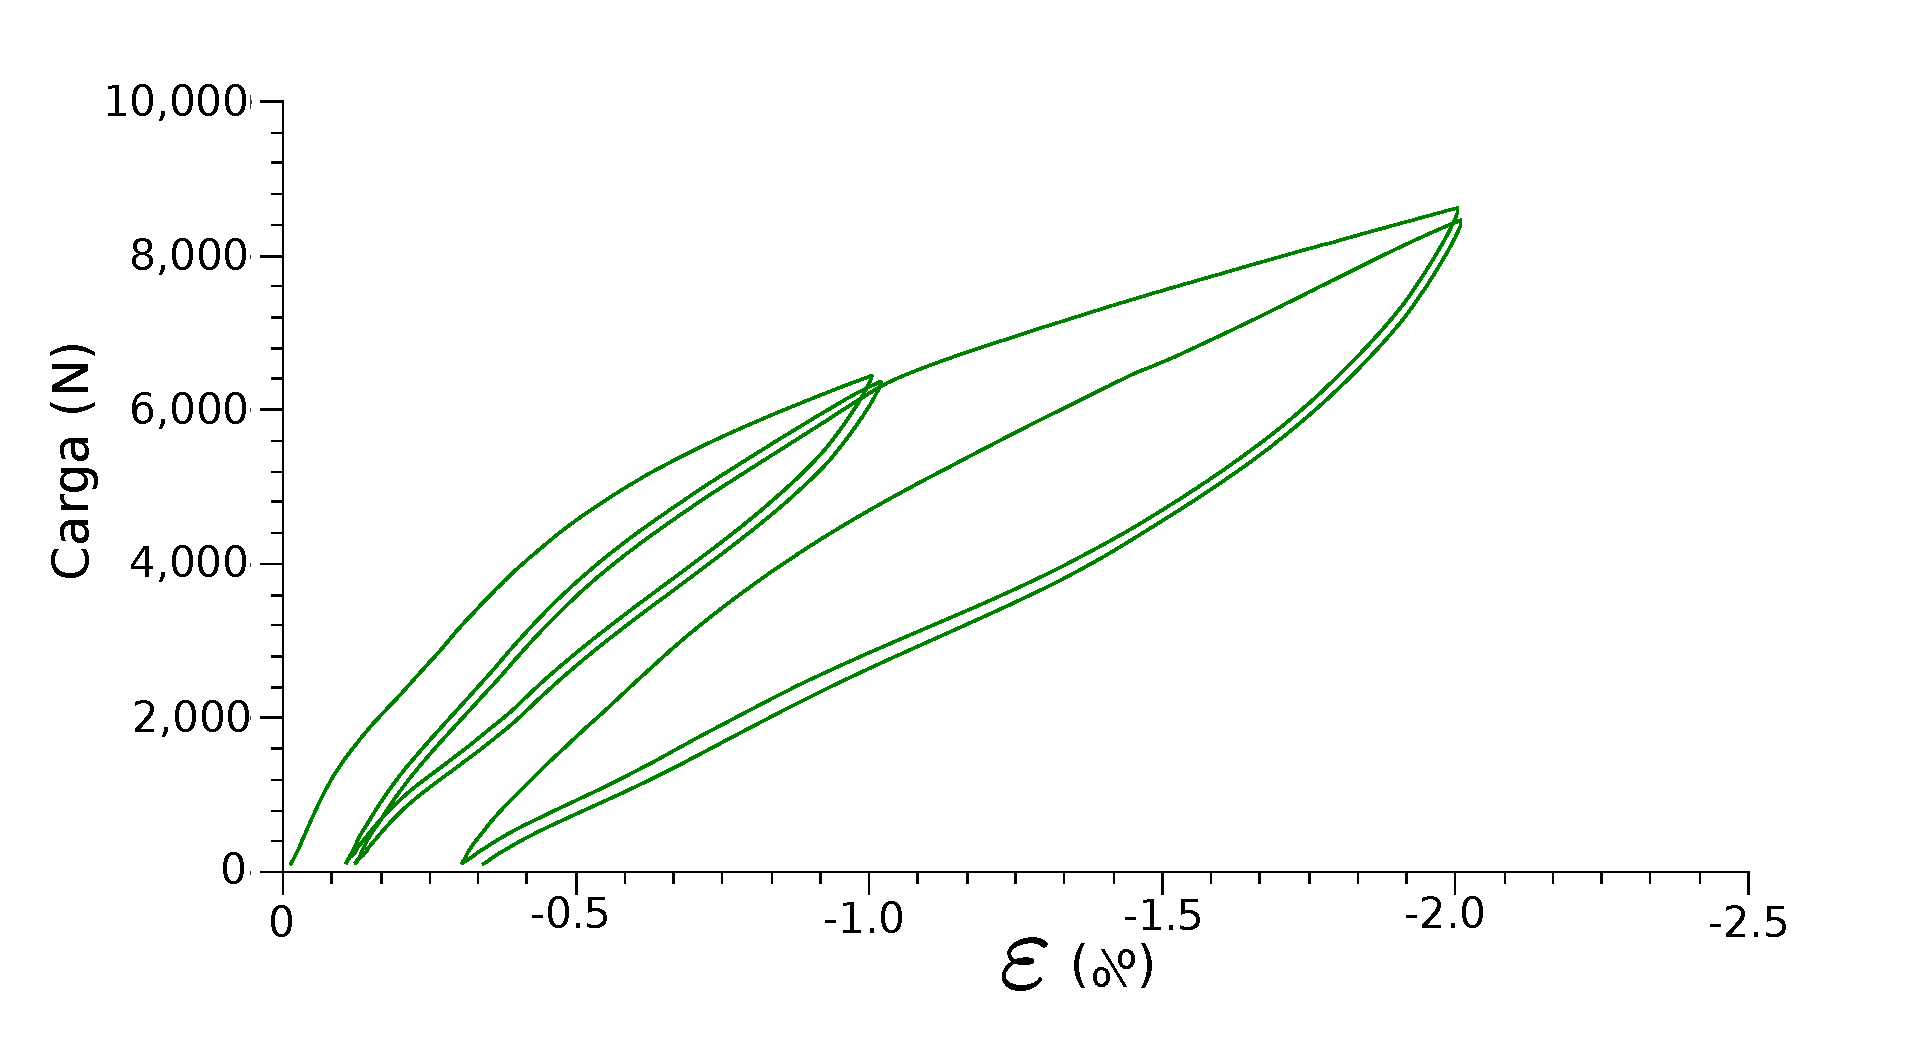
\includegraphics[width=\columnwidth]{img/intro/Graph533b.eps}
% \end{columns}
\vspace{-.5cm}
\begin{tiny}
\hspace{2cm} Esponja elastoplástica  \hspace{2.5cm} Esponja pseudoelástica
\end{tiny}

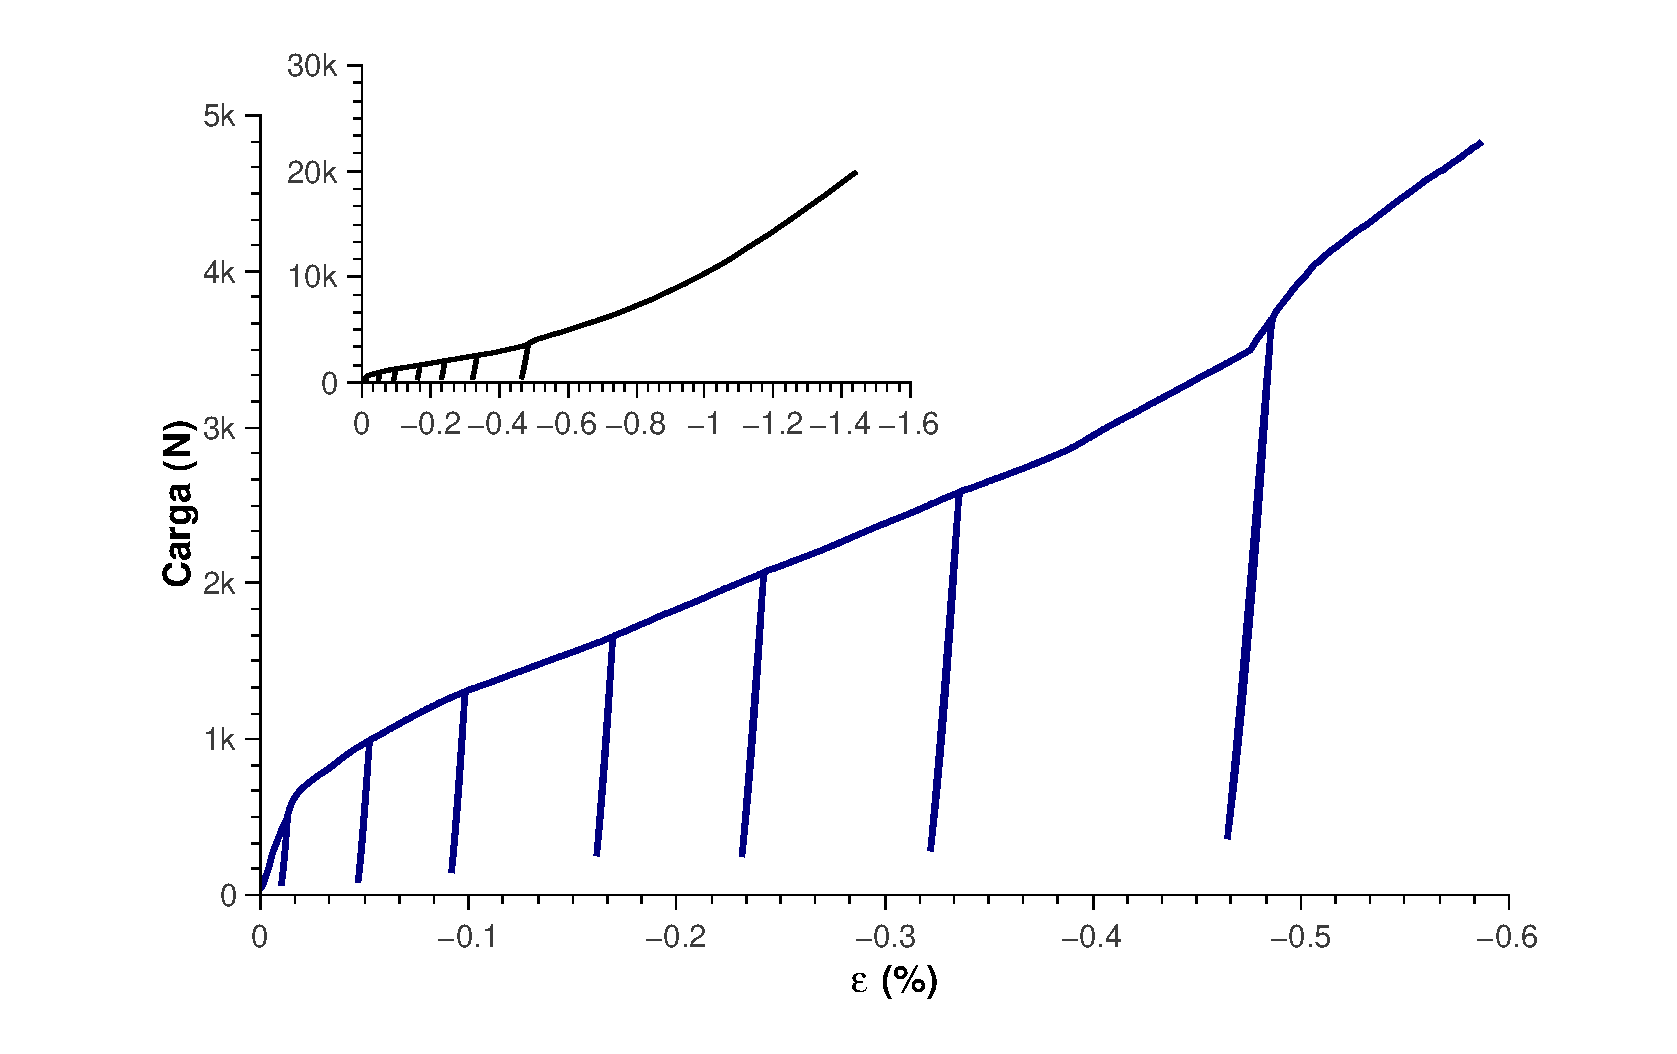
\includegraphics[width=0.5\textwidth]{img/intro/Cucompararesponja.eps}
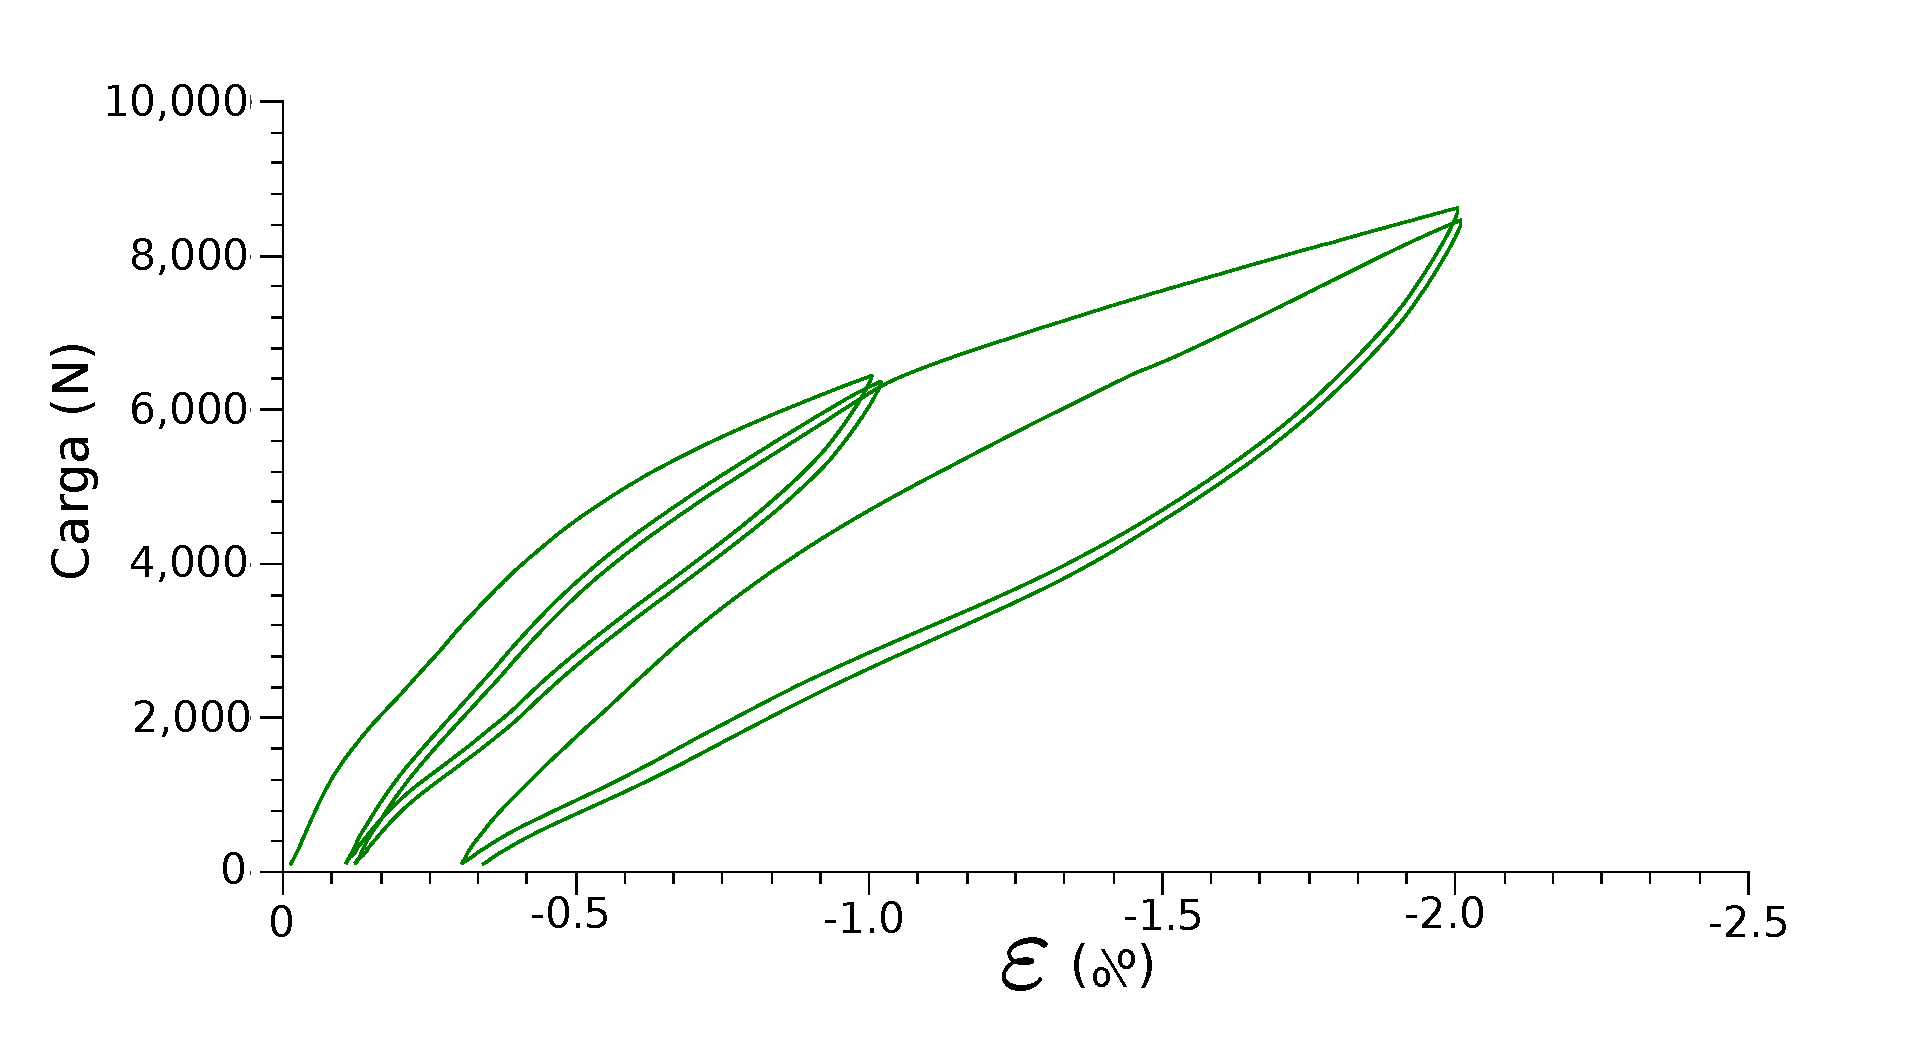
\includegraphics[width=0.5\textwidth]{img/intro/Graph533b.eps}

 \begin{itemize}
  \item {Gran capacidad de deformación}
  \item {Recuperación de la forma inicial}
  \item {Disipación de energía}
 \end{itemize}

\end{frame}

%*************************

% 
% \begin{frame}
%  \begin{itemize}
%   \item Memoria de forma
%   
%  
%  \end{itemize}
%  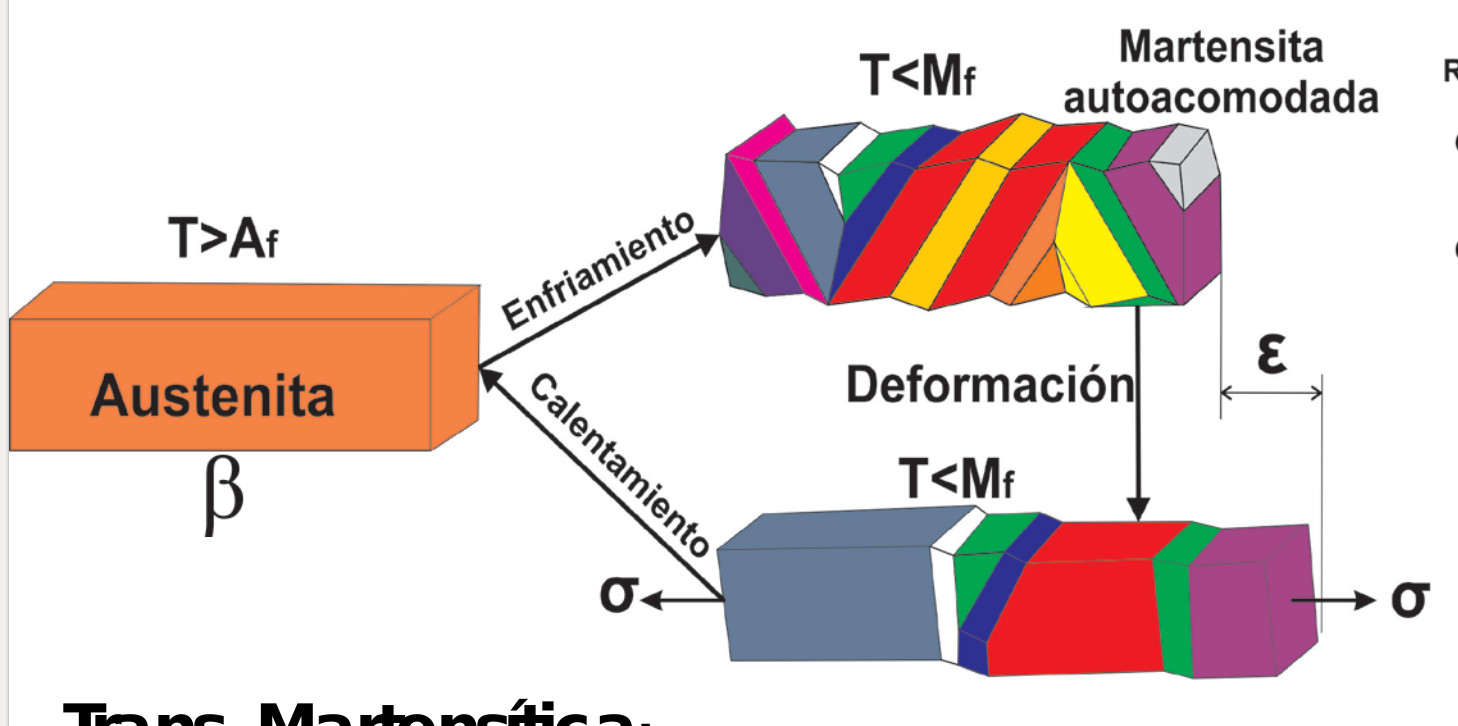
\includegraphics[width=0.8\textwidth]{img/intro/memoria.jpg}
% \end{frame}

% ******************
% 
% \begin{frame}
% 
% 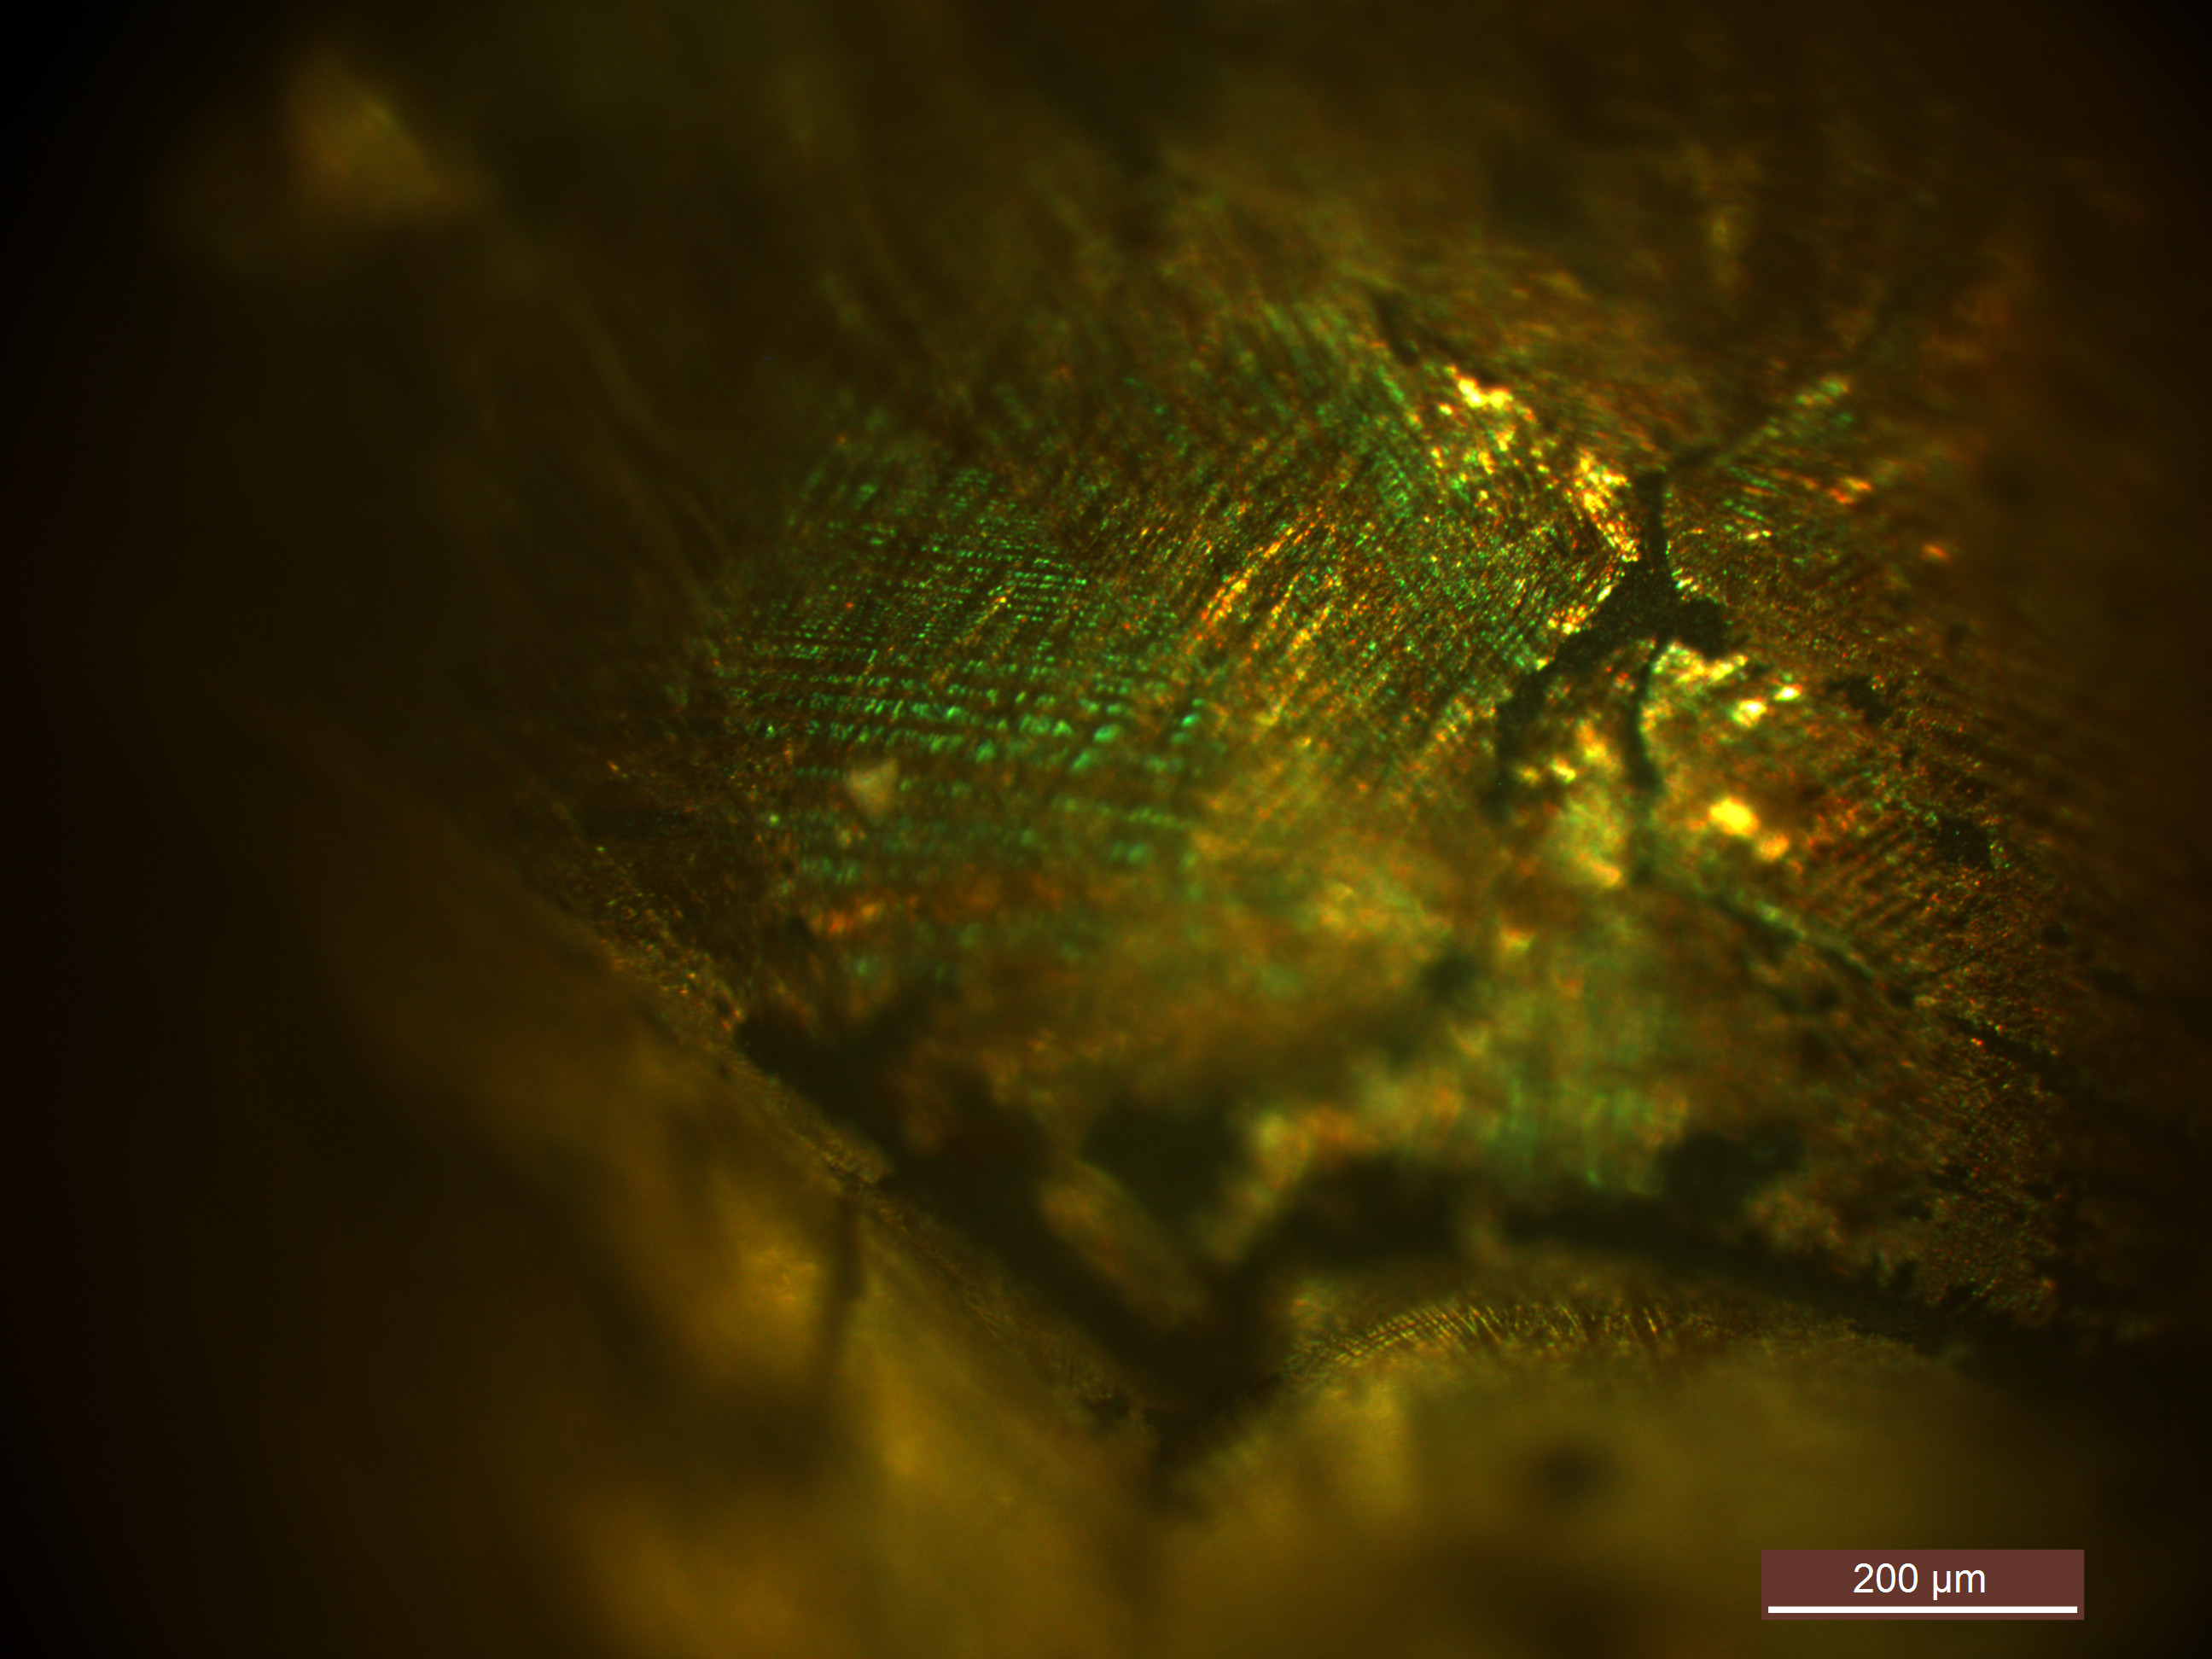
\includegraphics[width=0.4\textwidth]{img/intro/EspAMicro4.jpg}
% 
% 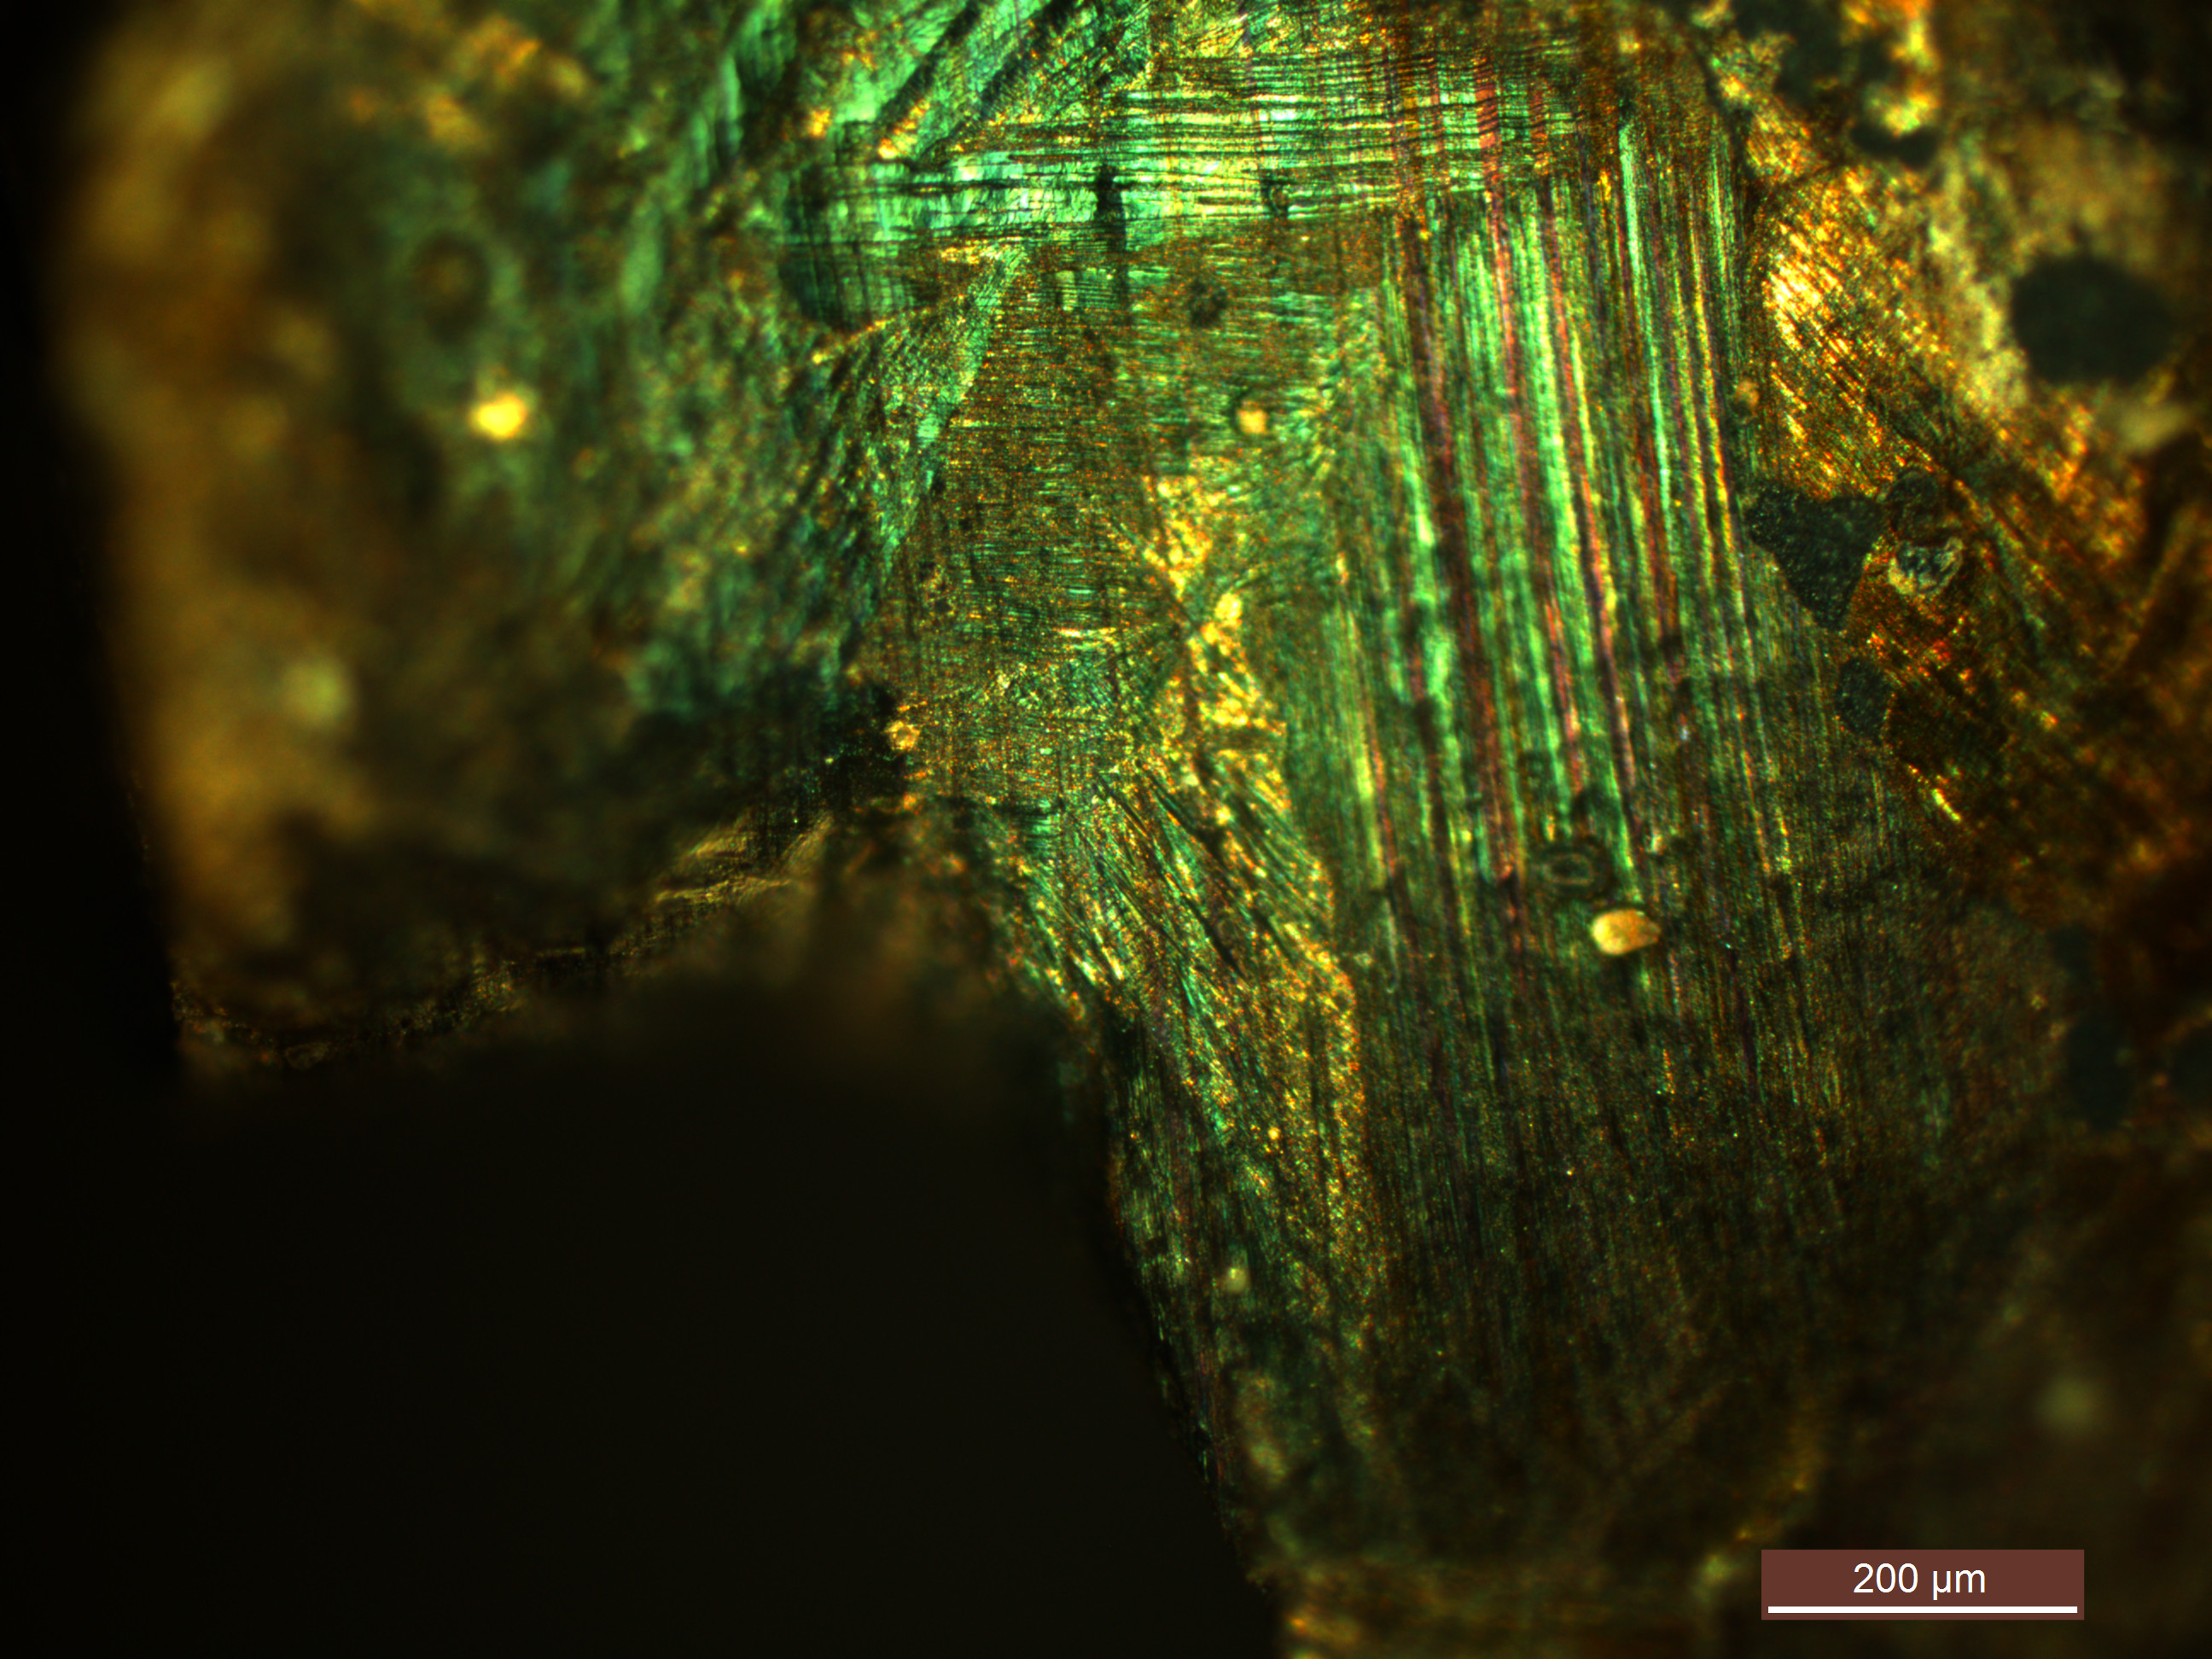
\includegraphics[width=0.4\textwidth]{img/intro/EspAMicro2.jpg}
% 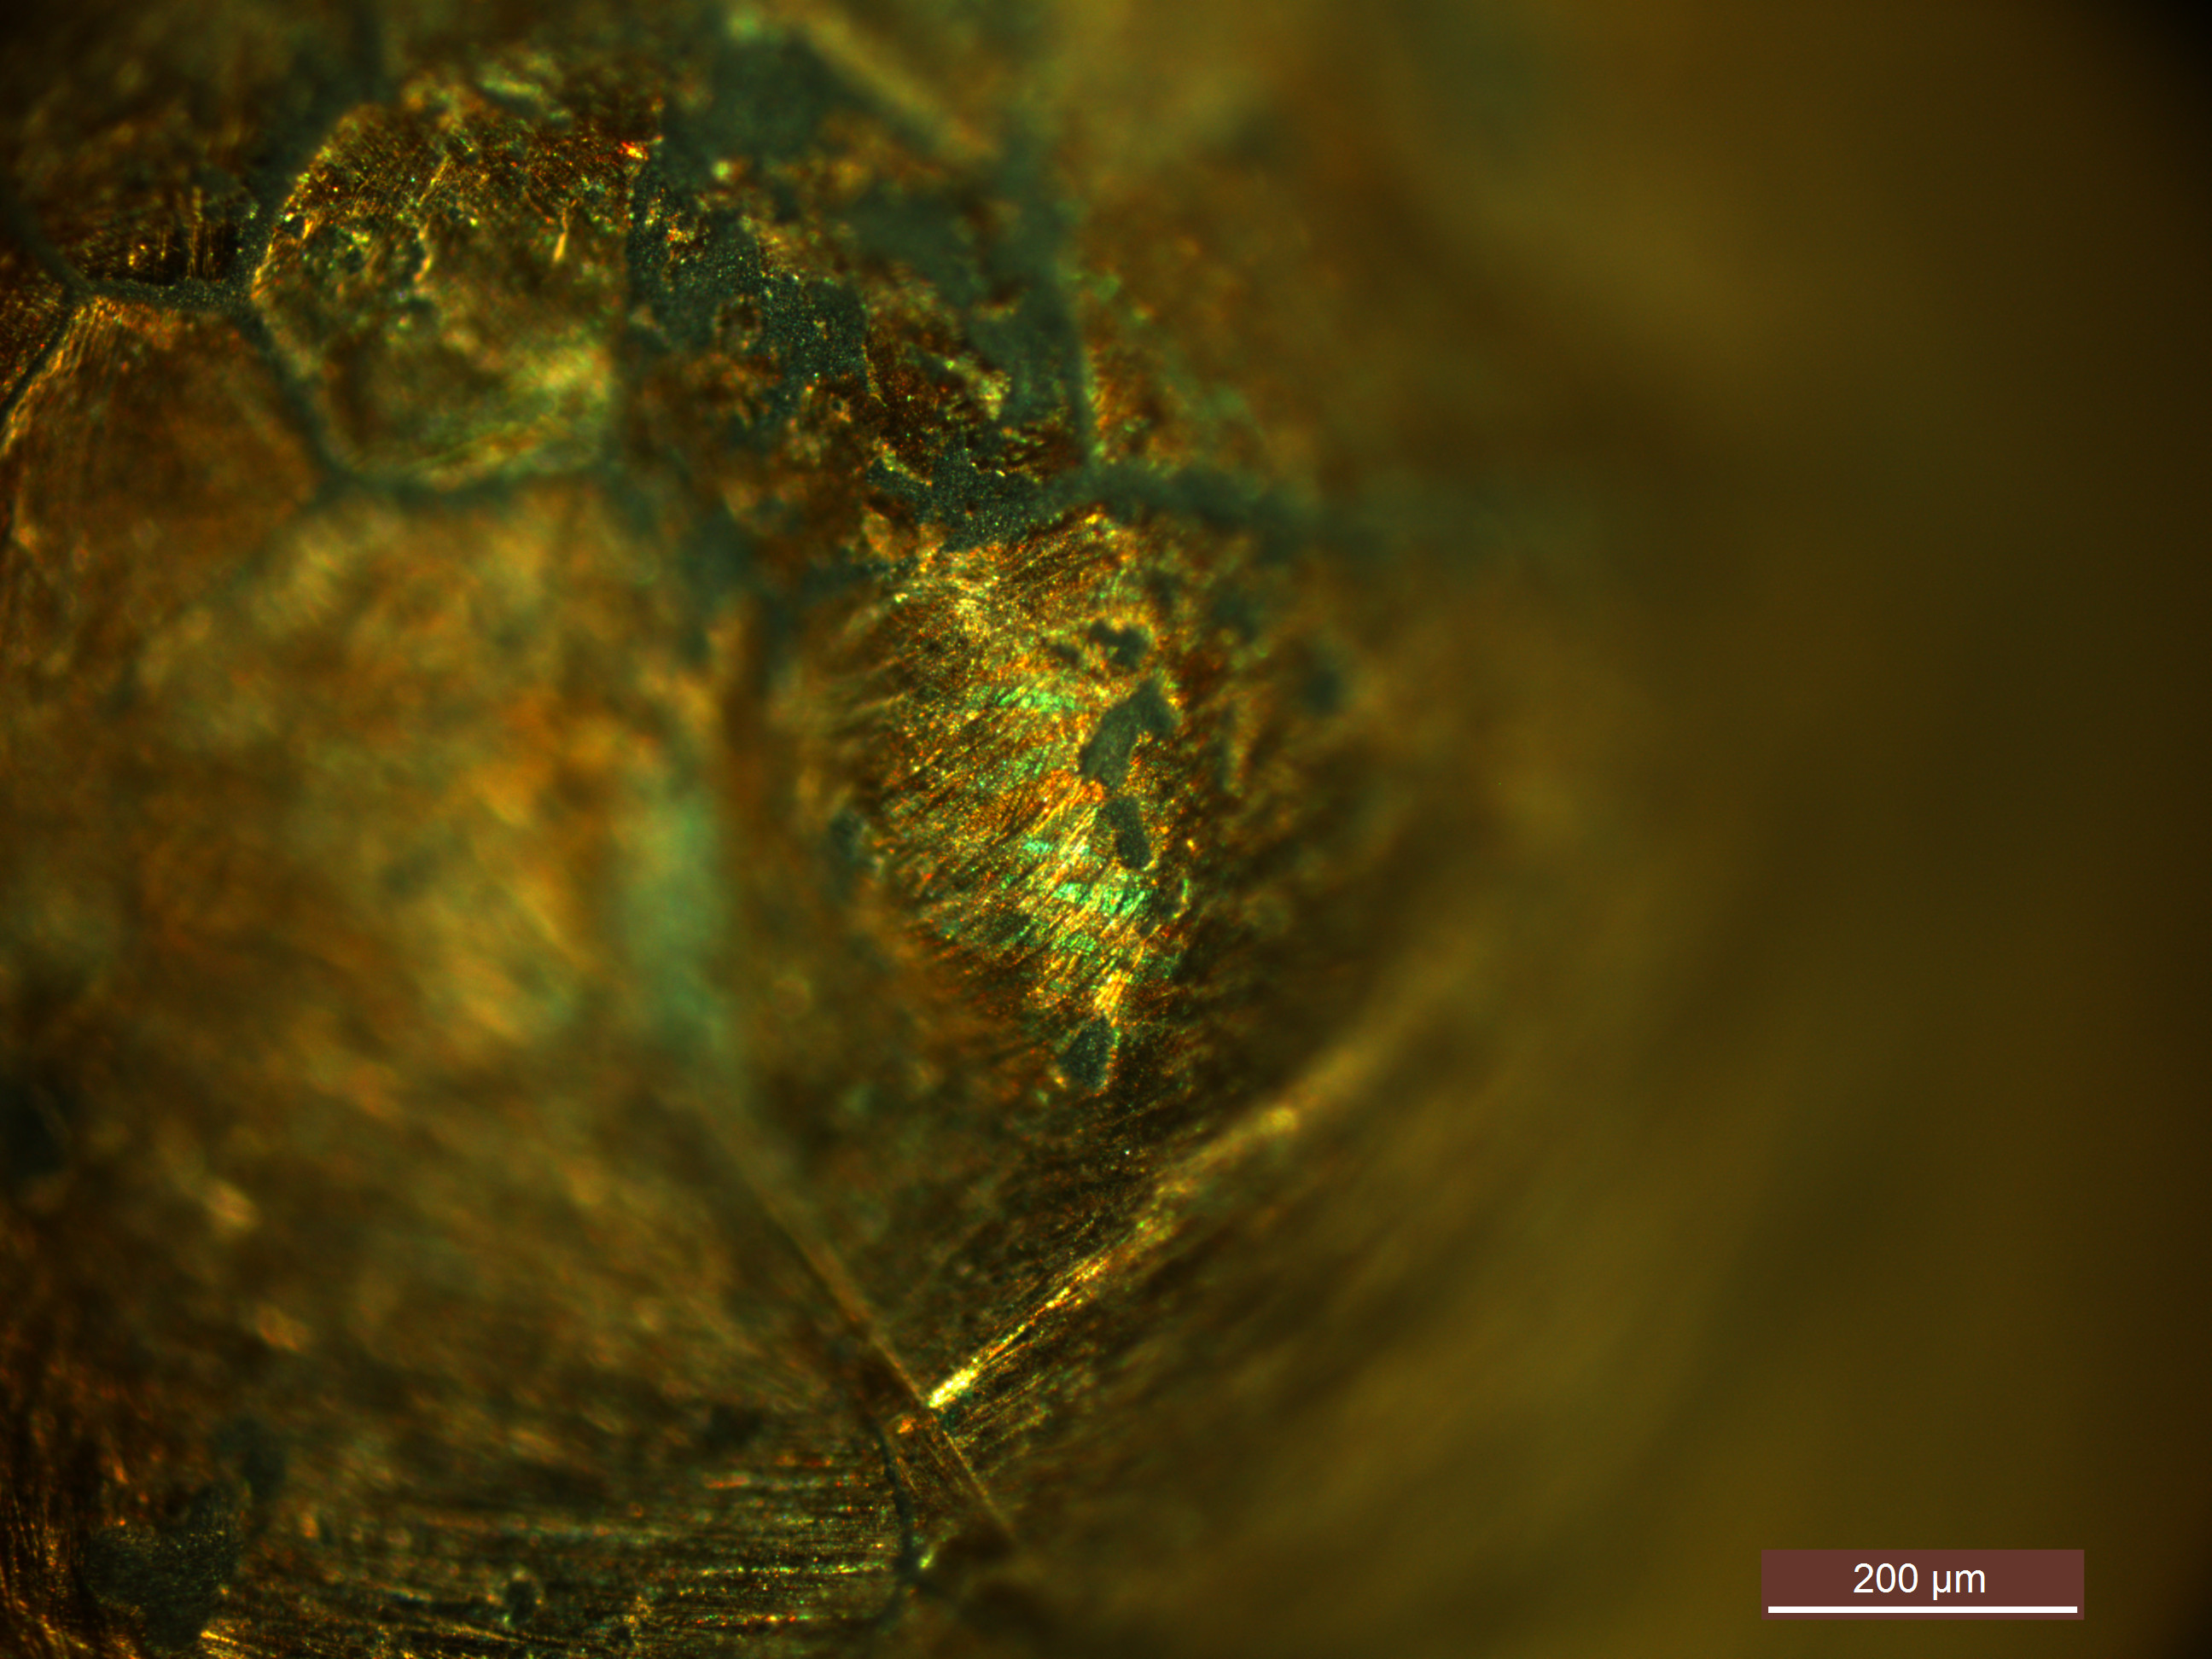
\includegraphics[width=0.4\textwidth]{img/intro/EspAMicro3.jpg}
%  
% \end{frame}
%%%%%%%%%%%%%%%%%%%%%%%%%%%%%%%%%%%%%%%%%%%%%%%%%%%%%%%%%%%%%%%%%%%%%%%%%%%%%%%%%%%%%%%%%%%%%%%%%55
% \begin{frame}
% Anisotropía elástica lleva a fisuras intergranulares 
% \end{frame}



% ******************

% \begin{frame}
%  Esponjas pseudoelásticas
% \end{frame}

% *************************************************************PREPARACION DE LA ALEACIÓN*********************************************************

% \begin{frame}
%  
%  \frametitle{Preparación de la aleación}
%  
%  \begin{itemize}
%  \item \textbf{Cu:} $50 \%$ ácido nítrico (al $65 \%$) - $50 \%$ agua
%  \item \textbf{Zn:} $60 \%$ ácido nítrico (al $65 \%$) - $40 \%$ agua
%  \item \textbf{Al:} $60 \%$ agua - $30 \%$ ácido clorhídrico (al 37 \%) - $10 \%$ ácido fluorhídrico (al $48 \%$)
% \end{itemize}
% 
% \vfill
% 
% \begin{center}
% 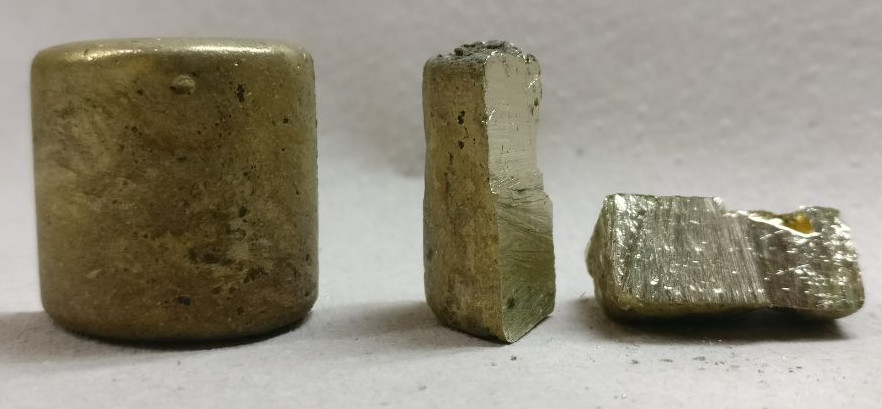
\includegraphics[width=0.4\textwidth]{img/proceso/lingote.jpg}
% \end{center}
% \end{frame}
% %%%%%%%%%%%%%%%%%%%%%%%%%%%%%%%%%%%%%%%%%%%%%%%%%%%%%%%%%%%%%%%%%%%%%%%%%%%%%%%%%%%%%%%%%%%%%%%%%%%%%%%%%%%%%55


\begin{frame}
\frametitle{Método de fabricación de esponjas pseudoelásticas}



\begin{columns}
\column{0.4\textwidth}
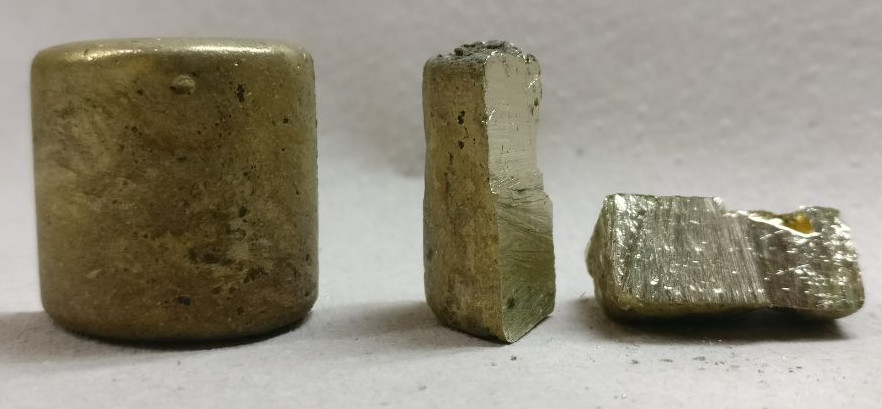
\includegraphics[width=0.8\textwidth]{img/proceso/lingote.jpg}

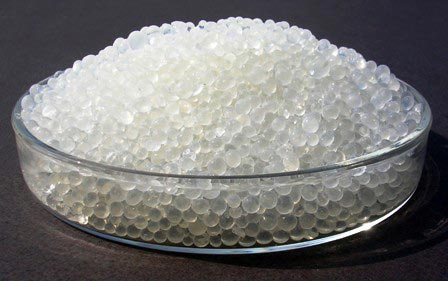
\includegraphics[width=0.8\textwidth]{img/proceso/silica.jpg}

\column{0.2\textwidth}

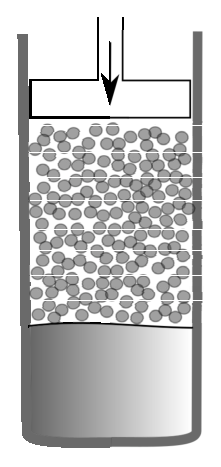
\includegraphics[width=0.8\textwidth]{img/proceso/proceso1.eps}

%\includegraphics[width=0.05\textwidth]{img/proceso/flecha.eps}
\column{0.2\textwidth}

\includegraphics[width=0.8\textwidth]{img/proceso/proceso2.eps}

%\includegraphics[width=0.05\textwidth]{img/proceso/flecha.eps}

%\column{0.25\textwidth}
%\includegraphics[width=0.8\textwidth]{img/proceso/proceso3.eps}
\end{columns}
%\end{center}
\end{frame}


\begin{frame}

\frametitle{Método de fabricación de esponjas pseudoelásticas}

\begin{center}
\begin{columns}
\column{0.30\textwidth}
\includegraphics[width=0.8\textwidth]{img/proceso/proceso1.jpg}
\column{0.30\textwidth}
\includegraphics[width=0.8\textwidth]{img/proceso/proceso2.jpg}
\column{0.30\textwidth}
\includegraphics[width=0.8\textwidth]{img/proceso/proceso3.jpg}
\end{columns}
\vspace{1cm}

 \begin{center}
 \begin{small}
\begin{tabular}{@{}llll@{}}  \toprule
%Muestra  &   $\% pp$ $AlB_2$ & Método \\ \midrule
% \alert<1>{Botón 1} & 18,866         & 0,005             & I      & Inducción\\
% \alert<2>{Botón 2} & 18,564         & 0,5               & I      &Resistivo\\
% \alert<3>{Botón 3} & 14,129         & 0,5               & II     &Resistivo \\
% \alert<4>{Botón 4} & 18,383         & 0,5               & II     & Resistivo \\
Largo &     $35$ $mm$    \\
Diámetro  & $25$ $mm$   \\
Densidad específica  & $\sim$ $0,17$     \\
% & 0,005             & Molienda     \\
\bottomrule
\end{tabular}
\end{small}
 \end{center}



\end{center}
\end{frame}
%%%%%%%%%%%%%%%%%%%%%%%%%%%%%%%%%%%%%%%%%%%%%%%%%%%%%%%%%%%%%%%%%%%%%%%%%%%%%%%%%%%%%%%%%%%%%%%%%%%%%%%%%%%%%%%%%%%%%%%%%%%%%%%%%%%%%%%%%

\begin{frame}
\frametitle{Medición de la $M_s$}

\begin{columns}
\column{0.5\textwidth}
 \includegraphics[width=\textwidth]{img/proceso/esquema_medicion_ms.jpg}
\column{0.5\textwidth}
\includegraphics[width=\textwidth]{img/proceso/Ms1.eps}


 \end{columns}


 
\end{frame}

%%%%%%%%%%%%%%%%%%%%%%%%%%%%%%%%%%%%%%%%%%%%%%%%%%%%%%%%%%%%%%%%%%%%%%%%%%%%%%%%%%%%%%%%%%%%%%%%%%%%%%%%%%%%%%%%%%%%%%%%%%%%%%%%%%%%%%%%%%%%


\begin{frame}
\frametitle{Fractura Intergranular}


%\begin{multicols}{2}
\begin{center}
\begin{columns}
\column{0.50\textwidth}
\includegraphics[width=0.8\textwidth]{img/tamgrano/Esponjacompleta1.eps}
\column{0.50\textwidth}
\includegraphics[width=\textwidth]{img/tamgrano/Fisuras.eps}
\end{columns}
%\end{multicols}
\vspace{1cm}
 \begin{small}
Esponja de Cu-Zn-Al de concentración electrónica 1,48, densidad específica $0,16$, diámetro de $23,4$ $mm$ y poros entre $1,4$ y $2,8$ $mm$.
\end{small}
% ¿Podemos prevenir las fisuras intergranulares?
% 
% ¡Modifiquemos el tamaño de grano!
\end{center}

%  
% \alert<4>{Comportamiento mecánico de la estructura + transformaciones $=$ Muy complejo!!} $\rightarrow$ \alert<5>{buscamos método sencillo para entender lo que sucede y poder seguir la integridad estructural de la esponja.} 
\end{frame}


%\subsection{Tamaño de grano}

% ******************
% \begin{frame}
%  Introducción fractura intergranular
% \end{frame}

% ******************
% \begin{frame}
%  Principal método para refinar el tamaño de grano $\rightarrow$ Boro $\rightarrow$ $AlB_2$
% \end{frame}



%%%%%%%%%%%%%%%%%%%%%%%%%%%%%%%%%%%%%%%%%%%%%%%%%%%%%%%%%%%%%%%%%%%%%%%%%%%%%%%%%%%%



%%%%%%%%%%%%%%%%%%%%%%%%%%%%%%%%%%%%%%%%%%%%%%%%%%%  BOTONES  %%%%%%%%%%%%%%%%%%%%%%%%%%%%%%%




%%%%%%%%%%%%%%%%%%%%%%%%%%%%%%%%%%%%%%%%%%%%%%%%%%%%%%%%%%%%%%%%%%%%%%%%%%%%%%%%%%%%%%%%%%%%%%%%%%%%%%%%%%%%%%%%%%%%%%%%%%%%%%%%%%%%%%%%%%%
\begin{frame}
\frametitle{Reducción del tamaño de grano}
\begin{columns}
\column{0.70\textwidth}
\begin{block}{Métodos de refinamiento}
 \begin{itemize}
  \item Tratamientos termomecánicos
  \item Agentes refinadores
 \end{itemize}
\end{block}
\column{0.30\textwidth}
\begin{center}
\includegraphics[width=\columnwidth]{img/proceso/boton.jpg}

$\diameter \sim 20 mm$
\end{center}
\end{columns}

Principal agente refinador: $B$ $\rightarrow$ $AlB_2$

\vspace{0.5 cm}

Agregado de $AlB_2$ en fundición $\rightarrow$ No incorporación

\end{frame}

%%%%%%%%%%%%%%%%%%%%%%%%%%%%%%%%%%%%%%%%%%%%%%%%%%%%%%%%%%%%%%%%%%%%%%%%%%%%%%%%%%%%%%%%%%%%%%%%%%%%%%%%%%%%%%%%
\begin{frame}

\frametitle{Molienda Mecánica}

Refina y mezcla compuestos. Puede generar reacciones químicas y aumentar la solubilidad.

\textsc{Mecanismo:} Soldadura en frío, fractura y resoldadura de partículas

\begin{columns}
 \column{0.30\textwidth}
 \includegraphics[width=0.9\textwidth]{img/tamgrano/MoliendaBolas.jpg}
 \column{0.30\textwidth}
 \includegraphics[width=0.9\textwidth]{img/tamgrano/Polvo.png}
 \column{0.50\textwidth}
\begin{small}

 \begin{itemize}
 \item $8\ g$ de aleación 
 \item Refinador $AlB_2$
 \item 5 bolas de acero $\diameter\ 25\ mm$
 \item $5\ atm$ de argón
 \item $28\ hs$ de molienda.
\end{itemize}

\end{small}
\end{columns}
\vspace{0.5 cm}
\begin{small}
Fundición: Tubos de cuarzo con atmósfera de Ar.
\end{small}



 \end{frame}
% 
% 
% %%%%%%%%%%%%%%%%%%%%%%%%%%%%%%%%%%%%%%%%%%%%%%%%%%%%%%%%%%%%%%
% \begin{frame}
%  \frametitle{Disminución tamaño de grano}
% 
% \begin{small}
% \begin{tabular}{@{}lllllll@{}}  \toprule
% Muestra            & $Cu-Zn-Al (g)$ &   $\% pp$ $AlB_2$ & Método & Horno \\ \midrule
% % \alert<1>{Botón 1} & 18,866         & 0,005             & I      & Inducción\\
% % \alert<2>{Botón 2} & 18,564         & 0,5               & I      &Resistivo\\
% % \alert<3>{Botón 3} & 14,129         & 0,5               & II     &Resistivo \\
% % \alert<4>{Botón 4} & 18,383         & 0,5               & II     & Resistivo \\
% Clavo 1 & 8               & 0,5               & III    & Resistivo \\
% %Clavo 2 & 8               & 0,05              &III     & Resistivo \\
% %Clavo 3 & 8               & -                 & IV   & Resistivo \\
% %Clavo 4 & 8               & 0,005             &IV      & Resistivo \\
% \bottomrule
% \end{tabular}
% \end{small}
% 
% \begin{description}
% \item[Método III:] Molienda mecánica de aleación $+$ $AlB_2$ y prensado de pastillas
% \item[Método IV:] Molienda mecánica de aleación $+$ $AlB_2$
% \end{description}
% 
% \begin{center}
% \includegraphics[width=0.2\textwidth]{img/proceso/PastMolienda.jpg}
% \includegraphics[width=0.4\textwidth]{img/proceso/ClavoPolvo.jpg}
% \end{center}
% 
% 
%  \end{frame}
%%%%%%%%%%%%%%%%%%%%%%%%%%%%%%%%%%%%%%%%%%%%%%%%%%%%%%%%%%%%%%%%%%%%%%%%%%%%%%%%%%%%%%%%%%%%%%%%%%%%%%%%%%%%%%%%

\begin{frame}
 \frametitle{Reducción del tamaño de grano}

 \begin{center}
 \begin{small}
\begin{tabular}{@{}llllll@{}}  \toprule
Muestra  &   $\% pp$ $AlB_2$ & Método \\ \midrule
% \alert<1>{Botón 1} & 18,866         & 0,005             & I      & Inducción\\
% \alert<2>{Botón 2} & 18,564         & 0,5               & I      &Resistivo\\
% \alert<3>{Botón 3} & 14,129         & 0,5               & II     &Resistivo \\
% \alert<4>{Botón 4} & 18,383         & 0,5               & II     & Resistivo \\
Clavo 1  & 0,5               & Molienda $+$ Prensado \\
Clavo 2  & 0,05              & Molienda $+$ Prensado \\
Clavo 3  & -                 & Molienda     \\
Clavo 4  & 0,005             & Molienda     \\
\bottomrule
\end{tabular}
\end{small}
 \end{center}

% \begin{description}
% \item[Método III:] Molienda mecánica de aleación $+$ $AlB_2$ y prensado de pastillas
% \item[Método IV:] Molienda mecánica de aleación $+$ $AlB_2$
% \end{description}
\hfill
\begin{columns}
 \column{0.330\textwidth}
\includegraphics[width=0.8\textwidth]{img/proceso/PastMolienda.jpg}

$ \diameter_{Pastilla}$ $5$ $mm$

$L_{Pastilla}$ $5$ $mm$

\vspace{0.5 cm}
 \column{0.330\textwidth}
\includegraphics[width=0.6\textwidth]{img/tamgrano/ClavoMuestra.jpg}

$ \diameter_{Clavo}$ $6$ $mm$

$L_{Clavo}$ $40$ $mm$

$ \diameter_{Muestra}$ $4,5$ $mm$


\column{0.330\textwidth}
\includegraphics[width=0.9\textwidth]{img/proceso/ClavoPolvo.jpg}

$ \diameter_{Interno}$ $6$ $mm$

$L_{Polvo}$ $60$ $mm$


\end{columns}


 \end{frame}

 
 
 %%%%%%%%%%%%%%%%%%%%%%%%%%%%%%%%%%%%%%%%%%%%%%%%%%%%%%%%%%%%%%%%%%%%%%%%%%%%%%%%%% MICROGRAFIAS CLAVO 1
\begin{frame}
\frametitle{Micrografías Clavo 1}

\begin{columns}
 \column{0.6\textwidth}
\includegraphics[width=\columnwidth]{img/tamgrano/Clavo1_Foto2.jpg} 
 \column{0.4\textwidth}
 
 $ \diameter_{Clavo}$ $6$ $mm$
 
$L_{Clavo}$ $70$ $mm$
 
\end{columns}


\begin{columns}
 \column{0.4\textwidth}

\includegraphics[width=\textwidth]{img/tamgrano/Clavo2.png}
 \column{0.33\textwidth}
\includegraphics[width=\textwidth]{img/tamgrano/Clavo1Retro.png}
 \column{0.33\textwidth}
\includegraphics[width=\textwidth]{img/tamgrano/Clavo1Retro2.png}
\end{columns}

\end{frame}

 %%%%%%%%%%%%%%%%%%%%%%%%%%%%%%%%%%%%%%%%%%%%%%%%%%%%%%%%%%%%%%%%%%%%%%%%%%%%%%%%%%%%%%
 
 \begin{frame}
 
\frametitle{Tamaños de grano obtenidos}
\begin{center}
\includegraphics[width=0.9\textwidth]{img/tamgrano/TamGranos.eps} 

\begin{small}
\begin{tabular}{ll}  \toprule
Botón 1  & Fundición A+R \\
Clavo 1 y Clavo 2 & Molienda + pastillas A+R \\
Clavo 3 y Clavo 4 &  Molienda + A+R \\
Clavo 5  & Fundición A \\
\bottomrule
\end{tabular}
\end{small}

\end{center}


\end{frame}
 
 
%%%%%%%%%%%%%%%%%%%%%%%%%%%%%%%%%%%%%%%%%%%%%%%%%%%%%%%%%%%%%%%%%%%%%%%%%%



% \begin{frame}
%  \frametitle{Disminución del tamaño de grano}
% 
%  
%  \begin{small}
% \begin{tabular}{@{}llllll@{}}  \toprule
% Muestra            & $Cu-Zn-Al (g)$ &   $\% pp$ $AlB_2$ & Método \\ \midrule
% % \alert<1>{Botón 1} & 18,866         & 0,005             & I      & Inducción\\
% % \alert<2>{Botón 2} & 18,564         & 0,5               & I      &Resistivo\\
% % \alert<3>{Botón 3} & 14,129         & 0,5               & II     &Resistivo \\
% % \alert<4>{Botón 4} & 18,383         & 0,5               & II     & Resistivo \\
% Clavo 1 & 8               & 0,5               & Molienda $+$ Prensado \\
% Clavo 2 & 8               & 0,05              & Molienda $+$ Prensado \\
% Clavo 3 & 8               & -                 & Molienda     \\
% Clavo 4 & 8               & 0,005             & Molienda     \\
% \bottomrule
% \end{tabular}
% \end{small}
% 
% 
% % \begin{description}
% % \item[Método III:] Molienda mecánica de aleación $+$ $AlB_2$ y prensado de pastillas
% % \item[Método IV:] Molienda mecánica de aleación $+$ $AlB_2$
% % \end{description}
% \hfill
% \begin{columns}
%  \column{0.330\textwidth}
% \includegraphics[width=0.8\textwidth]{img/proceso/PastMolienda.jpg}
%  \column{0.330\textwidth}
% \includegraphics[width=0.7\textwidth]{img/tamgrano/ClavoMuestra.jpg}
% \column{0.330\textwidth}
% \includegraphics[width=0.9\textwidth]{img/proceso/ClavoPolvo.jpg}
% \end{columns}
% 
% 
%  \end{frame}

% 
% 
% 
%  \begin{frame}
%  
% \frametitle{Tamaños de grano obtenidos}
% \begin{center}
% \includegraphics[width=\textwidth]{img/tamgrano/TamGranos.eps} 
% \end{center}
% 
% 
% \end{frame}


%%%%%%%%%%%%%%%%%%%%%%%%%%%%%%%%%%%%%%%%%%%%%%%%%%%%%%%%%%%%%%%%%%%%%%%%%%%%%%%%%%%%%%%%%%%%%%%%%%%%%%%%%%%%%%%%%

\begin{frame}
\frametitle{Ciclos de Compresión de los Clavos Fabricados}

\begin{block}{Compromiso:}
\begin{itemize}
 \item Buena pseudoelasticidad
 \item Menor susceptibilidad a roturas por fractura intergranular
\end{itemize}
\end{block}

% \begin{columns}
% \column{0.33\textwidth}
% \includegraphics[width=\columnwidth]{img/tamgrano/Clavo3Comp.eps}
% \column{0.33\textwidth}
% \includegraphics[width=\columnwidth]{img/tamgrano/Clavo4Comp.eps}
% \column{0.33\textwidth}
% \includegraphics[width=\columnwidth]{img/tamgrano/Clavo5Comp.eps}
% \end{columns}

 \includegraphics[width=0.33\textwidth]{img/tamgrano/Clavo3Comp.eps}
 \includegraphics[width=0.33\textwidth]{img/tamgrano/Clavo4Comp.eps}
 \includegraphics[width=0.33\textwidth]{img/tamgrano/Clavo5Comp.eps}

Fabricación de esponjas implica múltiples fundiciones de la aleación: Molienda + $0,005\%$ $AlB_2$

\end{frame}

  

%%%%%%%%%%%%%%%%%%%%%%%%%%%%%%%%%%%%%%%%%%%%%%%%%%%%%%%%%%%%%%%%%%%%%%%%%%%%%%%%%%%%%
% \begin{frame}
% \frametitle{Aumento del tamaño de grano}
% 
% \begin{columns}
% \column{0.40\textwidth}
% \includegraphics[width=0.8\textwidth]{img/tamgrano/brigdman.jpg}
% \includegraphics[width=0.4\textwidth]{img/tamgrano/EspCuarzo.jpg}
% \column{0.50\textwidth}
% \includegraphics[width=0.9\textwidth]{img/tamgrano/EspRota.jpg}
% 
% \end{columns}
% \end{frame}

%***************************



%%%%%%%%%%%%%%%%%%%%%%%%%%%%%%%%%%%%%%%%%%%%%%%%%%%%%%%%%%%%%%%%%%%%%%%%%%%%%%%%%%%%%%%%%%%%%%%%%%%%%%%%%%%%%%%%

\begin{frame}

\frametitle{Evaluación de la integridad estructural y seguimiento de la transformación}
\begin{columns}
\column{0.50\textwidth}
\begin{center}
¿Qué ocurre?

\vspace{0.2cm}

\includegraphics[width=0.6\textwidth]{img/resistencia/QuePasa.jpg}
\end{center}

\column{0.50\textwidth}
Procesos de transformación...
\vspace{0.2cm}

\includegraphics[width=0.5\textwidth]{img/intro/EspAMicro2.jpg}
 
Integridad estructural...
\vspace{0.2cm}

\includegraphics[width=0.5\textwidth]{img/intro/EsponjaA_005.jpg}
% \begin{itemize}
%  \item Deformación
%  \item Transformación martensítica
%  \item Pseudoelasticidad
%  \item Integridad estructural
% \end{itemize}

\end{columns}

\end{frame}



%%%%%%%%%%%%%%%%%%%%%%%%%%%%%%%%%%%%%%%%%%%%%%%%%%%%%%%%%%%%%%%%%%%%%%%%%%%%%%%%%%%%%%%%%%%%%%%%%%%%%%%%%%%%%%%%%

\begin{frame}
\frametitle{Método cuatro puntas}

% \begin{columns}
%  \column{0.5\textwidth}
%  \centering
% \includegraphics[width=\columnwidth]{img/resistencia/CuatroPuntas1.eps}
% 
% \includegraphics[width=\columnwidth]{img/intro/RvsTClavo5.eps}
% 
%  \column{0.5\textwidth}
%  \centering
% \includegraphics[width=\columnwidth]{img/resistencia/cpfoto.png}
% 
% \includegraphics[width=\columnwidth]{img/resistencia/Ciclos.eps}
% 
%  \end{columns}

% \begin{equation*}
% V^+= V_A +I^+ . R - V_B 
% \end{equation*}
% \begin{equation*}
%  V^-= V_A +I^- . R - V_B 
% \end{equation*}
% \begin{equation*}
%  V^+ - V^-= [I^+ + I^-] R \longrightarrow R=\frac{V^+ - V^-}{(I^+ + I^-)}
% \end{equation*}
% \begin{equation*}
%  \rho = R . \frac{A}{l} \label{resist} 
% \end{equation*}
\begin{center}
\includegraphics[width=1\textwidth]{img/resistencia/cuatro_puntas.png}
\end{center}
\end{frame}

%%%%%%%%%%%%%%%%%%%%%%%%%%%%%%%%%%%%%%%%%%%%%%%%%%%%%%%%%%%%%%%%%%%%%%%%%%%%%%%%%%%%%%HISTERESIS
% 
% \begin{frame}
% 
% 
% \frametitle{Transformación Martensítica Inducida Térmicamente }
% 
% \begin{figure}
% \begin{tikzpicture}
% 
% \node[anchor=south west,inner sep=0] (image) at (0,0) {\includegraphics[width=0.8\textwidth]{img/intro/RvsTClavo5.eps}};
% 
% 
% \node (I) at (2.5,5) {};
% \node (II) at (4.2,5) {};
% 
% \node[align=right] (It)   at (2.5,-0.1) {$M_{f}$};
% \node[align=right] (IIt)  at (4.2,-0.1) {$M_{s}$};
%  
% \path[->]<1-> (I) edge [green, dashed, thick] (It);
% \path[->]<1-> (II) edge [green, dashed, thick] (IIt);
% 
% \end{tikzpicture}
% \end{figure}
% \end{frame}
% 
% 
% %%%%%%%%%%%%%%%%%%%%%%%%%%%%%%%%%%%%%%%%%%%%%%%%%%%%%%%%%%%%%%%%%%%%%%%%%%%%%%%%%%%%%%%%%%%%%%%%%%%%%%%%%%%%%%%%
% \begin{frame}
%   \frametitle{Primeras Mediciones}
%   \includegraphics[width=0.95\textwidth]{img/resistencia/Ciclos.eps}
% 
% \end{frame}
% 
% %%%%%%%%%%%%%%%%%%%%%%%%%%%%%%%%%%%%%%%%%%%%%%%%%%%%%%%%%%%%%%%%%%%%%%%%%%%%%%%%%%%%%%%%%%%%%%%%%%%%%%%%%%%%%%%%%%%%%%%%%%%%%%%%%%
% 
% \begin{frame}
% 
% - Resistencia varía en la transformación martensítica
% 
% - Tensiones aplicadas modifican esta variación
% 
% \end{frame}



\begin{frame}

\frametitle{Mediciones realizadas}
%         \includegraphics[width=0.4\textwidth]{img/resistencia/EjTensionDef.eps}
% %        \includegraphics[width=\textwidth]{Img/resistencia/Ejblanco.jpg}
% \newline
%         \includegraphics[width=0.4\textwidth]{img/resistencia/EjTempDef.eps}
% \includegraphics[width=0.4\textwidth]{img/resistencia/EjTempRes.eps}
% 

\includegraphics[width=\textwidth]{img/resistencia/EjEnsayos.eps}

\end{frame}



%%%%%%%%%%%%%%%%%%%%%%%%%%%%%%%%%%%%%%%%%%%%%%%%%%%%%%%%%%%%%%%%%%%%%%%%%%%%%%%%%%%%%%%%%%%%%%%%%%%%%%%%%%%%%%%
% 
% \begin{frame}
% \frametitle{Ejemplo de Como se Tomaron los valores de resistencia}
%         \includegraphics[width=0.5\textwidth]{img/resistencia/ExpRes.eps}
%         \includegraphics[width=0.7\textwidth]{img/resistencia/ExpStrain.eps}
% \end{frame}
% 


%%%%%%%%%%%%%%%%%%%%%%%%%%%%%%%%%%%%%%%%%%%%%%%%%%%%%%%%%%%%%%%%%%%%%555
% \begin{frame}
% \frametitle{Muestras analizadas}
%  Foto de muestras cilíndricas y clavo
% \end{frame}

%%%%%%%%%%%%%%%%%%%%%%%%%%%%%%%%%%%%%%%%%%%%%%%%%%%%%%%%%%%%%%%%%%%%%%%%%%%%%%%%%%%%%%%%%%%%%%%%%%%%%%%%%%%%%%%%
\begin{frame}

\frametitle{Variación en la Resistencia por Compresión}

\begin{figure}
\begin{tikzpicture}

\node[anchor=south west,inner sep=0] (image) at (-10,7.8) {\includegraphics[width=0.2\textwidth]{img/tamgrano/antes.eps}};
\node[anchor=south west,inner sep=0] (image) at (-5,7) {\includegraphics[width=0.25\textwidth]{img/tamgrano/despues.eps}};
 
\draw[green, very thick, dashed] (-9.4,3.8) -- (-1.8,3.8) -- (-1.8,4.9) -- (-9.4,4.9) -- (-9.4,3.9);

\node[align=left] (It)   at (-8.8,6.5) {$ R_0= \rho \frac{l_0}{A_0}$};

\node[align=left] (It)   at (-3.5,6.5) {$l=l_0 * (1+ \varepsilon)$};
\node[align=left] (It)   at (-3.5,5.5) {$A=\frac{A_0}{(1+ \varepsilon)^2}$};

\node[align=left] (It)   at (-5.6,4.4) {$R= \rho \frac{l}{A} = \rho (1+\varepsilon)^2 \frac{l_0}{A_0} = (1+\varepsilon)^2 R_0 $};

%= \rho f^2 \frac{l_0}{A_0}$};

\end{tikzpicture}
\end{figure}
\begin{tiny}
 Suponemos V=cte
\end{tiny}


\end{frame}



%%%%%%%%%%%%%%%%%%%%%%%%%%%%%%%%%%%%%%%%%%%%%%%%%%%%%%%%%%%%%%%%%%%%%%%%%%%%%%%%%%%%%%%%%%%%%%%%%%%%%%%%%%%%%%%%%%%%%%%%%%%%%%%%%%%%%
%  \begin{frame}
%  
%  \frametitle{Variación en la Resistencia por Compresión y Transformación}
%  
%  \begin{figure}
% \begin{tikzpicture}
% 
% \node[anchor=south west,inner sep=0] (image) at (-10,7.5) {\includegraphics[width=0.2\textwidth]{img/tamgrano/antes.eps}};
% \node[anchor=south west,inner sep=0] (image) at (-5,7) {\includegraphics[width=0.2\textwidth]{img/tamgrano/despuesM.eps}};
%  
% \draw[green, very thick, dashed] (-9,3.4) -- (-1.4,3.4) -- (-1.4,4.5) -- (-9,4.5) -- (-9,3.5);
% 
% \node[align=left] (It)   at (-8.6,6.5) {$ \rho_M =f \rho_A$};
% \node[align=left] (It)   at (-8.6,5.5) {$R_M^0 =fR_A$};
% 
% \node[align=left] (It)   at (-3.5,6.5) {$ {R_M}=f'R_A $};
% \node[align=left] (It)   at (-3.5,5.5) {$R_M=R_M^0 (1+\varepsilon)^2 = f' R_A$};
% 
% \node[align=left] (It)   at (-5.3,4) {$ R_M^0 (1+\varepsilon)^2 = f'R_A \quad \rightarrow \quad f' = f (1+\varepsilon)^2  $};
% 
% \end{tikzpicture}
% \end{figure}
% \end{frame}
%  
 
\begin{frame}
 \frametitle{Variación en la Resistencia por Compresión y Transformación}

\begin{columns}
\column{0.40\textwidth}
\includegraphics[width=\textwidth]{img/resistencia/Resistencia.eps}
\column{0.50\textwidth}
$ \rho_M =f \rho_A$

$R_M^0 =fR_A$
\vspace{0.5cm}

$ {R_M}=f'R_A $

\vspace{0.5cm}

$R_M=R_M^0 (1+\varepsilon)^2 = f' R_A$

\vspace{0.5cm}

$ R_M^0 (1+\varepsilon)^2 = f'R_A$  
\vspace{0.5cm}
\begin{center}
\begin{block}{\quad $f' = f (1+\varepsilon)^2$}
\end{block}
\end{center}
\end{columns}
\end{frame}
 
 
 
% ******************
% 
% \begin{frame}
% Solo transformación:
% \begin{equation*}
%   \rho_M =f \rho_A
% \end{equation*}
% \begin{equation*}
%  R_M^0 =fR_A   
%  % \longrightarrow    \rho_M=f\rho_A 
% \end{equation*}
% \begin{equation*}
%  {R_M}=f'R_A 
% \end{equation*}
% donde $f'$ es el factor que relaciona las resistencias en un experimento real. Como $R_M=R_M^0 (1+\varepsilon)^2 = f' R_A$ se llega a:
% \begin{equation*}
%  R_M^0 (1+\varepsilon)^2 = f'R_A
% \end{equation*}
% \begin{equation*}
% f' = f (1+\varepsilon)^2  \label{fprima}
% \end{equation*}
% Esta ecuación relaciona los valores de resistencia al transformar, tomando en cuenta los cambios geométricos en la muestra. 
% 
% \end{frame}



%%%%%%%%%%%%%%%%%%%%%%%%%%%%%%%%%%%%%%%%%%%%%%%%%%%%%%%%%%%%%%%%%%%%%%%%%%%%%%%%%%%%%%%%%%%%%%%%%%%%%%%%%%%%%%%%%

\begin{frame}
 \frametitle{Resultados obtenidos}
 \begin{figure}
 \includegraphics[width=0.9\textwidth]{img/resistencia/PoliMono3.eps}
% \caption{Gráficos obtenidos al realizar ciclos de compresión de una esponja de Cu-Zn-Al hasta $-2\%$ de deformación. Abajo se muestra un gráfico de la deformación en función del tiempo y arriba los correspondientes valores de resistencia. } 
 \end{figure}
 \begin{center}
$f' = f (1+\varepsilon)^2$ 
\end{center}
 
 
%  \begin{multicols}{2}
%  
% \begin{table} 
% \tiny
% \begin{tabular}{@{}llllll@{}} \toprule
% Tensión ($MPa$) & $\varepsilon$ ($\%$) &  $f'=\frac{R_M}{R_A}$\\ \midrule
%  0        &  0.76   & 1.27\\
%  1.93       &  0.37   & 1.28\\
%  17.4      &  -7.60  & 1.15\\
%  31.0      &  -7.90  & 1.17\\
%  46.5     &  -8.00  & 1.17  \\
%  Referencia    & 8.00  &  1.73   \\
%  \bottomrule
% \end{tabular}
%  \caption{Monocristal}
% %Resultados obtenidos al realizar ciclos térmicos de transformación con distintas cargas aplicadas con un monocristal de Cu-Zn-Al. En la primera columna se muestran las cargas aplicadas que se mantuvieron constantes durante cada ciclo de transformación, $\varepsilon$ es la deformación máxima registrada por el extensómetro al transformar completamente a martensita, $f=\frac{R_M}{R_A}$ es el cociente entre la resistencia en estado martensítico y el estado austenítico.}
% \end{table}
% 
%  
% \begin{table}
% \tiny
% \begin{center} 
% \begin{tabular}{@{}llllll@{}} \toprule
% Tensión (Mpa) & $\varepsilon$ ($\%$) &  $f'=\frac{R_M}{R_A}$\\ \midrule
%  0        &  -0.10   & 1.30\\
%  0       &  -0.60   & 1.27 \\
%  0      &  -0.50   & 1.28 \\
%  2.04      &  -0.90  & 1.27\\
%  18.4    &  -1.60  & 1.24 \\
% 32.7      &  -2.60 & 1.21\\
%  49.1     &  -2.50  & 1.23   \\
%  \bottomrule
% \end{tabular}
%  \caption{Policristal}
% %Resultados obtenidos al realizar ciclos térmicos de transformación con distintas cargas aplicadas con un policristal de Cu-Zn-Al. En la primera columna se muestran las cargas aplicadas que se mantuvieron constantes durante cada ciclo de transformación, $\varepsilon$ es la deformación máxima registrada por el extensómetro al transformar completamente a martensita, $\frac{R_M}{R_A}$ es el cociente entre la resistencia en estado martensítico y el estado austenítico. También se esquematiza que $f$ corresponde a la pendiente de la recta.}
% \end{center}
% \end{table}
%  
% \end{multicols}
 
 
\end{frame}

%%%%%%%%%%%%%%%%%%%%%%%%%%%%%%%%%%%%%%%%%%%%%%%%%%%%%%%%%%%%%%%%%%%%%%%%%%%%%%%%%%%%%%%%%%%%%%%5








%%%%%%%%%%%%%%%%%%%%%%%%%%%%%%%%%%%%%%%%%%%%%%%%%%%%%%%%%%%%%%%%%%%%%%%%%%%%%%%%%%%%%%%%%%%%%%%%%%%%%%%55
\begin{frame}

\frametitle{Mediciones con esponja}

\begin{center}
\includegraphics[width=0.7\textwidth]{img/resistencia/Histeresis2.eps}
\end{center}

\end{frame}


\begin{frame}
 
 \frametitle{Rotura de Esponjas}
 
  \begin{figure}
\begin{tikzpicture}

\node[anchor=south west,inner sep=0] (image) at (-10.2,3) {\includegraphics[width=0.4\textwidth]{img/resistencia/EsqEsp.eps}};
\node[anchor=south west,inner sep=0] (image) at (-5.2,3) {\includegraphics[width=0.4\textwidth]{img/resistencia/EsqEspRota.eps}};

\node (It) at (-8.2,2) {$A_0$};
\node (IIt) at (-3.2,2) {$A_i = ?$};
\node (IIIt) at (-3.2,1) {$a_i=\frac{A_0}{A_i}$};

%\path[->]<1-> (IIt) edge [green, thick] (IIIt);


\end{tikzpicture}
\end{figure}
 
 
\end{frame}


% % ******************
% \begin{frame}
% 
%  
%  \begin{figure}
% \begin{tikzpicture}
% 
% %\draw[green, very thick, dashed] (-1.5,-0.5) -- (-1.5,4);
% 
% %\node[anchor=south west,inner sep=0] (image) at (-5.5,-1) {\includegraphics[width=0.7\textwidth]{img/intro/CuZn.png}};
% 
% \node (I) at (0,0) {};
% \node (II) at (5, 0) {};
% \node (III) at (1.5, 1) {};
% \node (It)   at (0, 2) {$R^{A} _i$};
% \node (It)   at (0.5, 2) {$=$};
% \node[fill=green!20,anchor=base] (It)  at (2,2) {$\rho^A \frac{L_0}{A_i}(1-b_i) $};
% \node (IIIt) at (3.5,2) {$+$};
% \node[fill=blue!20,anchor=base] (IIt) at (4.6,2) {$\rho^M \frac{L_0}{A_i}b_i$};
% \node (IIIIIt) at (5.6,2) {$=$};
% \node (IIIIIIt) at (7.5,2) {$\rho^A \frac{L_0}{A_i} [1+ b_i (f-1)]$}; 
% \node (IIIIIt) at (0,0) {Austenita}; 
% \node (IIIIIt) at (6,0) {Martensita retenida}; 
% 
%  \path[->]<1-> (I) edge [green, thick, bend left] (It);
%  \path[->]<1-> (II) edge [green, thick, bend right] (IIt);
% % \path[->]<1-> (IIIt) edge [blue,very thick] (IIIIt);
% % \path[->]<1-> (IIt) edge [blue, thick] (IIIIIt);
% %\path[->]<1-> (IIt) edge [dashed] (IIIIIt);
% 
% \node (IIIIIIt) at (7.5,2) {Estado inicial};
% 
% \end{tikzpicture}
% \end{figure}
% \end{frame}
 
%%%%%%%%%%%%%%%%%%%%%%%%%%%%%%%%%%%%%%%%%%%%%%%%%%%%%%%%%%%%%%%%%%%%%%%%%%%%%%%%%%%%%%%%%%%%%%%%%%%%%5



 
 
 
 
 



%%%%%%%%%%%%%%%%%%%%%%%%%%%%%%%%%%%%%%%%%%%%%%%%%%%%%%%%%%%%%%%%%%%%%%%%%%%%%%%%%%%%%%%%%%%%%%%%%%%%%%5


\begin{frame}

\frametitle{Área Específica y Martensita Retenida}
\begin{columns}
\column{0.40\textwidth}
Área específica: $a_i=\frac{A_0}{A_i}$ 

\vspace{0.5cm}
Martensita retenida $b_i$

\vspace{0.5cm}
$f=\rho^M / \rho^A$

\vspace{0.5cm}
%$R^A _i=\rho^A \frac{L_0}{A_i} [1+ b_i (f-1)]$

\begin{block}{$R^A _i=R^A _0 a_i [1+b_i (f-1)]$}
\end{block}


\begin{block}{$ R^M _i  = R^A _0 a_i f$}
\end{block}

\column{0.60\textwidth}

\includegraphics[width=\textwidth]{img/resistencia/Histeresis2.eps}

\end{columns}


\end{frame}


% ******************
%%%%%%%%%%%%%%%%%%%%%%%%%%%%%%%%%%%%%%%%%%%%%%%%%%%%%%%%%%%%%%%%%%%%%%%%%%%%%%%%%%%%%%%%%%%%%%%%%%%%%%

\begin{frame}

% \begin{tabular}{@{}lllll@{}} \toprule
% Muestra & $wt \% AlB_2$ & Método de fabricación & $\bar{tg} (mm)$ & $\sigma$ \\ \midrule
% austenítico &  -     & -   & 0.59  & 0.30   \\
% Ciclos térmicos    &  0,005 & I   & 0.31 & 0.22  \\
%  Ciclo térmico$4000$ $N$. &  0,50   & III & 0.16 & 0.08   \\
%  Ciclo térmico tensión aplicada &  0,05  & III & 0.10 & 0.05   \\
%  Ciclo térmico transformación &  -     & IV  & 0.11 & 0.05   \\
% 
% \bottomrule
% \end{tabular}

\frametitle{Ensayos realizados y resultados obtenidos}


% 
% \begin{enumerate}
%  \item Esponja en estado austenítico
%  \item Ciclo de transformación: $a_1 =1,009$ y $b_1=0,033 $
% \pause
% \vspace{0.5cm}
% \item Ciclo térmico de transformación con una tensión aplicada de $4000$ $N$.
%  \item Ciclo transformación: $a_2 =1,061$ y $b_2= 0,139$
%  \pause
% \vspace{0.5cm}
%  \item Ciclos de deformación hasta $2\%$
%  \item Ciclo de transforación: $a_3 =1,067$ y $b_3=0,166 $ 
% %  \pause
% %  \item Recocido a $800$ $^\circ C$
% %  \item $a_i =1,010$ y $b=0,044$
% 
% \end{enumerate}
\begin{small}

\begin{tabular}{@{}llllll@{}} \toprule
Condición de ensayo & $a_i$&  $b_i$\\ \midrule
Esponja en estado austenítico   &&\\
Ciclo térmico  & 1,009  & 0,033\\
Ciclo térmico con una tensión cte de $4000$ $N$  &&\\
Ciclo térmico &  1,061   & 0,139 \\
Ciclos de deformación hasta $2\%$ &&\\
Ciclo térmico  &  1,067  & 0,166  \\
 \bottomrule
\end{tabular}
\end{small}

$a_i$= Sección relativa

$b_i$= Fracción de martensita retenida

\end{frame}


%%%%%%%%%%%%%%%%%%%%%%%%%%%%%%%%%%%%%%%%%%%%%%%%%%%%%%%%%%%%%%%%%%%%%%%%%%%%%%%%%%%%%%%%%%%%%%%%%%%%%%%%%%%%%%%%
% \begin{frame}
% \frametitle{Ensayos realizados y resultados obtenidos}
% \begin{itemize}
%  \item Recocido a $800$ $^\circ C$
%  \item Ciclos de deformación hasta $2 \%$ 
%  \item $a_i =0,992$ y $b=0,029 $
%  \pause
%  \item Recocido a $800$ $^\circ C$
%  \item  $a_i =1,007$ y $b=0,054$
% \end{itemize}
% \end{frame}

%%%%%%%%%%%%%%%%%%%%%%%%%%%%%%%%%%%%%%%%%%%%%%%%%%%%%%%%%%%%%%%%%%%%%%%%%%%%%%%%%%%%%%%%%%%%%%%%%%%%%%%%%%%%%%%%
\begin{frame}
\frametitle{Recapitulación y conclusiones}
\begin{small}
\begin{itemize}
 \item A partir de los ensayos de compresión corroboramos que gran parte de las fallas se dan de forma intergranular. 
 \item A partir del uso de molienda mecánica se logró incorporar el $AlB_2$. 
 \item Logramos un refinamiento marcado del tamaño de grano de la aleación por medio del agregado de $AlB_2$.
 \item También encontramos el efecto refinador debido a la molienda mecánica.  
 \item Queda pendiente la utilización de este método para fabricar esponjas con menor tamaño de grano: \textbf{molienda mecánica + $B$ o $AlB_2$}
\end{itemize}
\end{small}

\end{frame}

%%%%%%%%%%%%%%%%%%%%%%%%%%%%%%%%%%%%%%%%%%%%%%%%%%%%%%%%%%%%%%%%%%%%%%%%%%%%%%%%%%%%%%%%%%%%%%%%%%%%%%%%%%%%%%%%
\begin{frame}
\frametitle{Recapitulación y conclusiones}
\begin{small}
\begin{itemize}
\item A partir de un método sencillo pudimos realizar el seguimiento de las transformaciones de fase y la integridad estructural de la esponja. 
\item Obtuvimos los parámetros relacionados a la martensita retenida y el área específica de la estructura.
\item Las mediciones pueden realizarse con equipos sencillos y sin sacar el dispositivo de funcionamiento.
\item Las aleaciones pseudoelásticas y las estructuras celulares fueron muy estudiadas en los últimos años. La combinación de ambas es muy prometedora y abre camino a muchas posibilidades que requerirán más estudio.
\end{itemize}
\end{small}
\end{frame}



\begin{frame}[standout]
 
 ¡Muchas gracias!

 \end{frame}















\appendix
% 
% \begin{frame}
\begin{frame}

\frametitle{Martensita retenida y rotura}

Resistencia inicial en estado austenítico sin rotura: 
\begin{equation*}
 R^A _0 = \rho^A \frac{L_0}{A_0}
\end{equation*}
Además $f$ relaciona las resistividades de la austenita y martensita:
\begin{equation*}
 f=\rho^M / \rho^A
\end{equation*}
Luego del ciclo $i$ de transformación:
\begin{equation*}
R^A _i=\rho^A \frac{L_0}{A_i}(1-b_i) + \rho^M \frac{L_0}{A_i}b_i = \rho^A \frac{L_0}{A_i} [1+ b_i (f-1)]
\end{equation*}

$0<b_i <1$ fracción de martensita retenida

\end{frame}

\begin{frame}
 \frametitle{Martensita retenida y rotura}
 
Cuando comienza a romperse, la resistencia será la inicial calculada $R^A_0$ por un factor relacionado con el área específica $A_0/A_i$:
\begin{equation*}
 R^A _0 = \rho^A \frac{L_0}{A_0}
\end{equation*}
\begin{equation*}
 R^A _i =\rho^A \frac{L_0}{A_i} [1+ b_i (f-1)]= R^A _0 \frac{A_0}{A_i} [1+b_i (f-1)]  %=R^A _0 a_i [1+b_i (f-1)]
\end{equation*}

\begin{block}{
 \begin{equation*}
 R^A _i = R^A _0 a_i [1+b_i (f-1)] 
 \end{equation*}
 }
\end{block}


\end{frame}

\begin{frame}

Si ahora comparamos le resistencia inicial en estado austenítico $R^A _0$ con la resistencia en estado martensítico luego del ciclo $i$ de transformación :
\begin{equation*}
 R^M _i = \rho ^M \frac{L_0}{A_i}
\end{equation*}
\begin{equation*}
 f=\rho^M / \rho^A \longrightarrow
 R^M _i = f R^A _0 \frac{A_0}{A_i} = R^A _0 a_i f 
\end{equation*}

\begin{block}{
\begin{equation*}
 R^M _i  = R^A _0 a_i f
\end{equation*}
 }
\end{block}

\end{frame}

% 
% 
% %  \begin{frame}
% % % 
% % \frametitle{Resultados de ${A_0}/A$ y $b$} 
% % 
% % EN VEZ DE LAS TABLAS VOY A PONER LOS DISTINTOS GRAFICOS DE LOS ENSAYOS PARA EXPLICAR MEJOR LA SECUENCIA DE LO QUE FUIMOS HACIENDO E INTERCALADO LOS VALORES DE B Y ROTURA.
% % 
% % \begin{multicols}{2}
% %   \begin{table} 
% %  \tiny
% %  \begin{center} 
% %   \begin{tabular}{@{}lllllll@{}} \toprule
% %   Esponja & Ensayo   &    $R^M$    &  $R^A$ &  $A_0/A$ \\ \midrule
% %   1   & 1       &  0.040  & 0.031 & 1.009  \\
% %   1   & 2       &  0.046  & 0.034 &  1.061  \\
% %   1   & 3       &  0.058  & 0.042 &  1.067  \\
% %   1   & 4     &  0.089  & 0.068 &  1.010 \\
% %   2   & 1     &  0.015  & 0.011 &  0.992  \\
% %   2   & 2    &  0.017  & 0.013 &  1.007   \\
% %   \bottomrule
% % % ************************************************   GRAFICOS ESPONJA D
% %   \end{tabular}
% % %\caption{Parámetro $A/A_0$ calculado para las esponjas de Cu-Zn-Al en distintos ensayos a partir de los datos obtenidos del gráfico. Se ve como con cada ensayo el área de la esponja disminuye respecto del área inicial.}
% % %\label{tab:A0Arotura}
% % \end{center}
% %   \end{table}
% % 
% % 
% % % ******************
% % 
% % 
% % \begin{table} 
% % \tiny
% % \begin{center} 
% % \begin{tabular}{@{}lllllll@{}} \toprule
% % Esponja &Ensayo   &    $R^M$    &  ${R^A}$ &  b \\ \midrule
% % 1 & 1       &  0.031  & 0.031   & 0.033  \\
% % 1 & 2       &  0.035  & 0.034  &  0.139  \\
% % 1 & 3       &  0.044  & 0.042  &  0.166  \\
% % 1 & 4      &  0.069 &	0.068 &	0.044 \\
% % 2 & 1      &  0.011 &	0.011 & 0.029 \\
% % 2 & 2      &  0.013 &	0.012 & 0.054\\
% %  \bottomrule
% % 
% %  \end{tabular}
% % %\caption{Valores de martensita retenida ($b$) obtenidos para las esponjas 1 y 2 de Cu-Zn-Al utilizando los valores del gráfico \ref{fig:RED_resultados} }
% % 
% % \end{center}
% % \end{table}
% % 
% % \end{multicols}
% % \end{frame}
% 
% % ******************%%%%%%%%%%%%%%%%%%%%%%%%%%%%%%%%%%%%%%%%%%%%%%%%%%%%%%%%%%%%%%%% BOTONES
% 
% \begin{frame}
%  Conclusiones
% \end{frame}
% 
% \begin{frame}
%  \frametitle{Disminución tamaño de grano}
% 
% \begin{small}
% \begin{tabular}{@{}lllllll@{}}  \toprule
% Muestra            & $Cu-Zn-Al (g)$ &   $\% pp$ $AlB_2$ & Método & Horno \\ \midrule
% \alert<1>{Botón 1} & 18,866         & 0,005             & 1      & Inducción\\
% \alert<2>{Botón 2} & 18,564         & 0,5               & 1      &Resistivo\\
% \alert<3>{Botón 3} & 14,129         & 0,5               & 2     &Resistivo \\
% \alert<4>{Botón 4} & 18,383         & 0,5               & 2     & Resistivo \\
% % Clavo 1 & 8 & - & - & 0,5 & 0,5 & III & Resistivo \\
% % Clavo 2 & 8 & - & - & 0,05 & 0,05 &III & Resistivo \\
% % Clavo 3 & 8 & - & - & - & - &  IV & Resistivo \\
% % Clavo 4 & 8 & - & - & 0,005 & 0,005 &IV & Resistivo \\
% \bottomrule
% \end{tabular}
% \end{small}
% 
% \begin{description}
% \alert<1,2>{\item[Método 1:] Aleación $+$ $AlB_2$ papel aluminio $+$ $Cu$} 
% \alert<3,4>{\item[Método 2:] Aleación $+$ $AlB_2$ $\rightarrow$  prensado de pastillas}
% \end{description}
% 
% \includegraphics[width=0.16\textwidth]{img/proceso/boton.jpg}
% \includegraphics[width=0.33\textwidth]{img/proceso/ampolla.jpg}
% \includegraphics[width=0.32\textwidth]{img/tamgrano/Esponjaypastillas.jpg}
% \includegraphics[width=0.175\textwidth]{img/proceso/PastViruta.jpg}
% 
% 
%  \end{frame}
% 
% %%%%%%%%%%%%%%%%%%%%%%%%%%%%%%%%%%%%%%%%%%%%%%%%%%%%%%%%%%%%%%%%%%%%%%%%%%% MICROGRAFIAS SEM DEL BOTON
% \begin{frame}
% 
% \includegraphics[width=\textwidth]{img/tamgrano/tamano_grano_l1b1.eps}
% 
% \end{frame}


\end{document}